% !TEX program = xelatex
% This is samplepaper.tex, a sample chapter demonstrating the
% LLNCS macro package for Springer Computer Science proceedings;
% Version 2.20 of 2017/10/04
%
\documentclass[runningheads]{llncs}
%\documentclass[draft,runningheads]{llncs}

%
\usepackage{graphicx}
\usepackage{dhucs-cmap}
\usepackage[hangul]{kotex}
%\SetHangulFonts{utgr}{utgt}{uttz}
\usepackage{tabularx} 
\usepackage{amsmath}
\usepackage{amssymb}
\usepackage{braket}
\usepackage{listings}
\usepackage{xcolor}
\usepackage{menukeys} 
\usepackage{pythonhighlight}
\usepackage{subfig}
\usepackage{setspace}
\usepackage{geometry}
\usepackage{color}
\usepackage{soul}
\usepackage{enumitem}
\usepackage{setspace}
\usepackage{tikz}
\usepackage{booktabs}
\usepackage{multirow}
\usepackage{arydshln}
\usepackage{float}
\usepackage{url}
\usepackage{adjustbox}
\usepackage{multirow}

\geometry{
  a4paper,
  left=2.5cm,
  right=2.5cm,
  top=2.5cm,
  bottom=2.5cm
}

\setstretch{1.1}

\raggedbottom

\makeatletter
\renewcommand*\l@section[2]
  {%
    \ifnum \c@tocdepth >\z@
      \addpenalty \@secpenalty
      \addvspace {1.0em \@plus \p@ }%
      \setlength \@tempdima {1.5em}%
      \begingroup
        \parindent \z@
        \rightskip \@pnumwidth
        \parfillskip -\@pnumwidth
        \leavevmode \bfseries
        \advance \leftskip \@tempdima
        \hskip -\leftskip
        #1\nobreak
        \hfil
        \nobreak
        \hb@xt@ \@pnumwidth {\hss #2\kern -\p@ \kern \p@ }%
        \par
      \endgroup
    \fi
  }

\makeatother

\makeatletter
\renewcommand\subsubsection{
  \@startsection{subsubsection}{3}{\z@}
  {-3.25ex\@plus -1ex \@minus -.2ex}
  {1.5ex\@plus .2ex}
  {\normalfont\normalsize\bfseries}%
}
\makeatother

\definecolor{codegreen}{rgb}{0.13, 0.55, 0.13}
\definecolor{codegray}{rgb}{0.5,0.5,0.5}
\definecolor{codepurple}{rgb}{0.58,0,0.82}
\definecolor{backcolour}{rgb}{0.95,0.95,0.92}

\lstdefinestyle{customc}{
	backgroundcolor=\color{backcolour},   
	commentstyle=\color{codegreen}\itshape,
	keywordstyle=\color{magenta},
	numberstyle=\tiny\color{codegray},
	stringstyle=\color{codepurple},
	basicstyle=\ttfamily\footnotesize,
	language=Python,
	basicstyle=\fontsize{7}{7}\ttfamily,
	breakatwhitespace=false,         
	breaklines=true,                 
	captionpos=b,                    
	keepspaces=true,                 
	numbers=left,                    
	numbersep=6pt,                  
	showspaces=false,                
	showstringspaces=false,
	showtabs=false,                  
	tabsize=2
}

\lstdefinestyle{customasm}{
	backgroundcolor=\color{backcolour},   
	belowcaptionskip=1\baselineskip,
	language=[x86masm]Assembler,
	basicstyle=\fontsize{7}{7}\ttfamily,
	commentstyle=\color{codegreen},
	keywordstyle=\color{black},
	identifierstyle=\color{black},
    captionpos=b,                    
	keepspaces=false,                 
	tabsize=2,
	numbers=left,
	numbersep=5pt,
	showspaces=false, 
	showtabs=false,
	numberstyle=\tiny\color{gray}
}

\hyphenpenalty=10000
\exhyphenpenalty=10000

\lstdefinestyle{custompython}{
  backgroundcolor=\color{backcolour},
  language=Python,
  basicstyle=\ttfamily\fontsize{7}{9}\selectfont,
  commentstyle=\color{codegreen}\itshape,
  keywordstyle=\color{blue}\bfseries,
  stringstyle=\color{codepurple},
  numbers=left,
  numbersep=6pt,
  numberstyle=\tiny\color{codegray},
  breaklines=true,            
  breakatwhitespace=true,     
  keepspaces=true,            
  columns=fullflexible,      
  showstringspaces=false,
  tabsize=2,
  captionpos=b,
  inputencoding=utf8,         
  extendedchars=true,
  upquote=true,
  literate={~}{{\textasciitilde}}1 % 
}

% Used for displaying a sample figure. If possible, figure files should
% be included in EPS format.
%
% If you use the hyperref package, please uncomment the following line
% to display URLs in blue roman font according to Springer's eBook style:
% \renewcommand\UrlFont{\color{blue}\rmfamily}

\newcommand{\eg}{{\em 예,}\xspace}
\newcommand{\ie}{{\em i.e.,}\xspace}
\newcommand{\etc}{{\em etc.}\xspace}
\newcommand{\quotes}[1]{``#1''}



\newcommand*\BC[1]{%
	\begin{tikzpicture}[baseline=(C.base)]
		\node[draw,circle,fill=black,inner sep=0.2pt](C) {\textcolor{white}{#1}};
\end{tikzpicture}}

\newcommand{\PP}[1]{\vspace{2pt}\noindent{\bf#1.}\xspace}

\begin{document}

%
\title{Aegis-UxV: 다중 도메인 국방 무인체계를 위한 도구 근거 RED/BLUE 에이전트}
%
%\titlerunning{Abbreviated paper title}
% If the paper title is too long for the running head, you can set
% an abbreviated paper title here
%

\author{BombTEE: 전형준, 권유정, 김민석, 백가현}
%
\authorrunning{성균관대학교 SecAI 연구실}
% First names are abbreviated in the running head.
% If there are more than two authors, 'et al.' is used.
%
\institute{성균관대학교 인공지능을 활용한 보안 연구실 (SecAI)}
%

\maketitle              % typeset the header of the contribution

% \setcounter{tocdepth}{2}
\setcounter{secnumdepth}{3}
\setcounter{tocdepth}{3} 
\tableofcontents

\vspace{30pt}
\listoffigures 

\vspace{20pt}
\listoftables

\newpage
% \section{요약 (Abstract)}

%  방산 무인체계 (UAV/UGV)와 이를 지휘하는 위성/BLOS(Beyond Line-Of-Sight) 데이터링크는 항상 적대적(contested)인 환경에서 운용된다는 점에서 민수용 드론 보안과 질적으로 다르다. 본 연구는 이 방산 특수성 --- BLOS 운용에 따른 경로상(on-path) 노출, 상시적인 GNSS 거부(denial), 인증·암호화가 없는 레거시 제어 프로토콜(MAVLink) --- 을 실제 ArduPilot SITL(ArduCopter/ArduRover) 및 userspace MITM MAVLink relay 위에서 실증한다. 실기체·실RF·GNSS 송신·root/kernel netem은 사용하지 않는 순수 시뮬레이션이다.

% 본 연구는 UAV·UGV·위성/BLOS 세 도메인에 걸쳐 \textbf{14개의 문서화된 공격}(RC/조향 오버라이드, MAVLink 명령 주입, GPS·지자기·IMU·기압 기만, GNSS 재밍, 미션·파라미터 변조, 데이터링크 열화/DoS/flooding/재전송)을 실제 운용 맥락 위에서 구현하고, 개별 공격을 넘어 \textbf{실측 공격 합성(kill-chain) 2건}(페일세이프 무력화 후 링크상실이 치명적 표류로 이어지는 KC-A, GPS+기압 복합 스푸핑이 직교합(quadrature) 관계의 3D 오차를 유발하는 KC-B)과, 실제 사건(이란 RQ-170 나포, 우크라이나 전자전, CVE-2020-10283)에 앵커링된 설계 수준 도트린 킬체인 2건을 제시한다. 모든 수치는 \emph{주입값(injected)}과 \emph{창발적 임무 결과(emergent outcome)}를 명시적으로 분리하여 보고한다 --- 동일한 GPS 40 m 기만이 정지 체공에서는 실제 이탈 0.009 m에 그치나 자율 항로 비행 중에는 18.31 m의 회랑 이탈을 유발하는 식이다.

% 방어 체계는 탐지(D2--D8 및 센서 교차검증)·예방·복구의 3층 구조를 가지며, 예방이 실제 SITL 액추에이션에 배선된 항목에만 정량 효과를 부여하는 5단계 정직성 태깅([LIVE]/[SIGN]/[NATIVE-FS]/[DETECT-ONLY]/[PROPOSED])을 도입한다. RC 오버라이드→BRAKE, GPS 기만→EKF 소스 전환, 명령/재전송/미션/파라미터 변조→MAVLink2 서명, 대역폭 flooding→rate-limit의 \textbf{5개 예방 메커니즘 클래스가 공격성공률(ASR)을 1.0에서 0.0으로 낮춤}을 인과적으로(dispatch on/off 대조) 실증하였으며, 자력계/IMU/기압계 스푸핑은 페일오버할 비오염 소스가 없다는 물리적 이유로 정직하게 탐지 전용(detect-only)임을 명시한다.

% AI 에이전트 계층에서는 도메인별 RED 계획 에이전트 3종(UAV/UGV/위성)과 단일 공유 BLUE 지휘관을 구축하였으며, 두 축 모두 실제 로컬 LLM CLI를 경계화된 서브프로세스로 호출해 실제 세션ID·비용이 기록되는 진성 LLM 추론을 수행한다. 탐지는 결정론적 도구가, 상관·귀속·대응 계획은 LLM이 담당하는 역할 분리 위에서, 지휘관 자신의 결정이 SITL 액추에이션을 구동하는 라이브 폐루프(ASR 1.0→0.0, n=3)를 실증하였다. 평가는 LLM이 LLM을 채점하는 순환을 배제한 결정론적 오라클 채점기로 수행하며, 독립 재판정을 통해 "도구가 탐지의 필요조건"이라는 초기 주장을 정직하게 철회·재정식화(일관성·감사가능성 우위로 재정의)하였다. 모든 결과는 시뮬레이션 전용·소표본(n≤5)이라는 한계 위에서 근거 경로와 함께 보고되며, 근거 없는 수치는 만들지 않고 미측정 또는 설계 수준으로 표기한다.

\section{요약 (Abstract)}

본 연구는 방위산업 분야의 국방 무인체계 (Defense Unmanned Systems) 가운데 무인항공기 (Unmanned Aerial Vehicle, UAV)와 무인지상차량 (Unmanned Ground Vehicle, UGV), 그리고 이들의 지휘통제 (Command and Control, C2) 메시지를 전달하는 위성 및 비가시선 (Beyond Line of Sight, BLOS) 데이터링크를 대상으로 한다. 
%
국방 무인체계의 C2 데이터링크는 민간용 드론 통신과 달리 적의 감시, 교란, 기만, 침투 가능성을 상시적으로 고려해야 하는 적대적 작전환경 (contested operational environment)을 전제로 하며, 이에 따라 위협 모델과 보안 검증 기준 또한 민간용 드론 보안과 구별한다. 
%
본 연구는 이러한 방산 특수성을 공격자가 BLOS C2 중계 경로상 위치를 확보한 조건, GNSS 거부 환경, 그리고 메시지 서명 및 별도 전송계층 암호화가 적용되지 않은 MAVLink 운용 구성이라는 세 가지 조건으로 정식화한다.
%
이를 위해 ArduPilot SITL (Software-in-the-Loop) 기반 ArduCopter 및 ArduRover 실험 환경을 구성한다.
%
위성/BLOS C2 데이터링크의 경로상 노출 조건은 사용자 공간에서 동작하는 MITM (Man-in-the-Middle) MAVLink 중계기 (relay)를 통해 모사한다. 
%
실험 범위는 순수 소프트웨어 시뮬레이션으로 한정하며, 실기체 및 실제 무선주파수 (Radio Frequency, RF) 송수신, GNSS 신호 송신, 루트 권한 (Root privilege), 커널 수준 네트워크 에뮬레이션 (kernel-level network emulation, netem)은 사용하지 않는다.


본 연구는 세 도메인에 걸쳐 14개의 공격 시나리오를 공격 모듈, 증거 하니스 주입, 사용자 공간 링크 에뮬레이션 방식으로 구현·재현한다. 공격군은 원격조종 (Radio Control, RC) 또는 조향 오버라이드, MAVLink 명령 주입, GPS (Global Positioning System) 기만, 자력계 (magnetometer) 기만, 관성측정장치 (Inertial Measurement Unit, IMU) 기만, 기압계 (barometer) 기만, GNSS 재밍 (jamming), 임무 변조, 파라미터 (parameter) 변조, 데이터링크 저하 (degradation), 서비스 거부 (denial of service, DoS), 플러딩 (flooding), 재전송 (replay) 공격을 포함한다. 
%
또한 개별 공격의 재현에 그치지 않고, 실험 측정 기반 연쇄 공격 1건과 복합 다중센서 공격 1건 (kill chain)을 제시한다. KC-A는 페일세이프 (failsafe) 무력화 이후 링크 상실이 치명적 표류로 이어지는 연쇄 효과를 다루며, KC-B는 GPS와 기압계의 복합 기만이 수평 및 수직 오차 성분의 직교합 (quadrature) 관계를 통해 3차원 위치 오차로 결합되는 현상을 다룬다. 
%
더 나아가 이란 RQ-170 나포, 우크라이나 전자전, CVE-2020-10283과 같은 공개 사례를 기준점으로 삼는 설계 수준의 독트린형 킬체인(doctrinal kill chain) 2건을 함께 제시한다. 
%
모든 정량 결과는 \emph{주입값 (injected value)}과 \emph{창발적 임무 결과 (emergent mission outcome)}를 명시적으로 분리하여 보고한다. 예를 들어 동일한 GPS 40 m 기만은 정지 체공 조건에서는 0.009 m 수준의 실제 이탈만 보이지만, 자율 항로 비행 조건에서는 18.31 m의 회랑 이탈로 이어지는 양상을 보인다.
%

본 연구의 방어 체계는 탐지 (detection), 예방 (prevention), 복구 (recovery)의 3층 구조로 구성한다. 
%
탐지 계층은 D2--D8 탐지기와 센서 교차검증 (sensor cross-validation)을 포함하며, 예방 계층은 실제 SITL 액추에이션에 배선된 항목에 한하여 정량적 방어 효과를 부여한다. 이를 위해 각 방어 결과를 [LIVE], [SIGN], [NATIVE-FS], [DETECT-ONLY], [PROPOSED]의 다섯 단계로 구분하는 근거 정직성 태깅 (evidence-honesty tagging)을 도입한다. 
%
구체적으로 RC 오버라이드 대응을 위한 BRAKE 전환, GPS 기만 대응을 위한 확장 칼만 필터 (extended Kalman Filter, EKF) 소스 전환, MAVLink 명령 주입 대응을 위한 MAVLink 2 서명, 재전송·미션·파라미터 변조 대응을 위한 MAVLink 2 서명 기반 검증, 대역폭 플러딩 대응을 위한 Rate-limit 적용을 예방 항목으로 정의한다. 
%
이들 능동 대응 항목은 평가된 폐루프 (closed loop) 구성에서 dispatch on/off 대조를 통해 해당 시나리오의 ASR을 1.0에서 0.0으로 낮췄다. 
%
반면 자력계, IMU, 기압계 기만은 페일오버 가능한 비오염 참조원이 없는 조건에서 예방 효과를 주장하지 않으며, 해당 항목을 탐지 전용 ([DETECT-ONLY])으로 분류한다.
%

AI 에이전트 계층에서는 도메인별 RED 계획 에이전트 3종, 즉 UAV RED, UGV RED, 위성/BLOS RED와 단일 공유 BLUE 커맨더 (BLUE commander)를 구성한다. 
%
RED와 BLUE는 모두 로컬 대규모 언어모델 명령줄 인터페이스 (local Large Language Model Command-Line Interface, local LLM CLI)를 권한 및 입출력 경계가 설정된 하위 프로세스로 호출하며, 각 호출은 실제 세션 식별자 (session ID)와 비용 로그를 남기는 실제 LLM 추론으로 수행한다. 
%
탐지는 결정론적 도구가 담당하고, 상관 (correlation), 귀속 (attribution), 대응 계획 (response planning)은 LLM이 담당하는 역할 분리 구조를 적용한다. 이 구조 위에서 BLUE 지휘관의 결정이 SITL 내 액추에이션을 직접 구동하는 실시간 폐루프 (live closed loop)를 검증하며, 해당 조건에서 ASR 1.0에서 0.0으로의 감소를 확인한다 (n=3). 
%
평가는 LLM이 LLM을 채점하는 순환 구조를 배제하고, 결정론적 오라클 채점기 (deterministic oracle scorer)를 통해 수행한다. 
%
또한 독립 재판정 절차를 통해 “도구가 탐지의 필요조건”이라는 초기 주장을 “도구는 탐지의 필요조건이 아니라 일관성, 재현성, 감사가능성 측면에서 우위를 제공하는 요소”로 재정식화한다. 모든 결과는 시뮬레이션 전용 환경과 소표본 조건 ($n \le 5$)이라는 한계를 전제로 제시하며, 각 수치에는 근거 경로를 함께 보고한다. 본 연구는 근거 없는 수치를 생성하지 않고, 미측정 항목과 설계 수준 항목을 명시적으로 구분한다.



\section{서론}

\subsection{배경: 방산 자율체계의 사이버 위협 지형}

무인항공기 (UAV), 무인지상차량 (UGV), 그리고 이들의 원격 지휘통제 (C2) 메시지를 전달하는 위성통신 (SATCOM) 기반 비가시선 (BLOS) C2 링크는 현대 방산 자율체계의 핵심 기반이다. 
%
방산 무인체계의 운용 환경은 민간용 드론과 본질적으로 다르다. 
%
가장 중요한 차이는 적의 감시, 교란, 기만, 침투 가능성을 기본 조건으로 삼는 적대적 작전환경 (Contested operational environment)에 있다. 본 연구는 이러한 적대성을 세 가지 방산 특수성으로 구조화한다.

\textbf{첫째}, BLOS 운용은 경로상 노출을 구조적으로 만든다. 
%
방산 정보·감시·정찰 (Intelligence, Surveillance, and Reconnaissance, ISR) 및 타격 UAV와 원거리 UGV는 가시선 밖에서 임무를 수행하므로, C2 링크가 위성 중계 또는 다중 홉 무선주파수 (Radio Frequency, RF) 경로에 의존한다. 이때 임차 트랜스폰더, bent-pipe 중계기, 지상 게이트웨이는 모두 관측, 지연, 손실, 변조가 가능한 개입 지점이 된다.
%
\textbf{둘째}, 글로벌 위성항법시스템 거부는 예외 상황이 아니라 상시 위협 조건이다. 현대 전장에서는 GPS 재밍과 기만이 항법 체계를 직접 겨냥한다. 
%
무인체계가 GNSS 단일 소스에 크게 의존할수록 위치·항법·시각 (positioning, navigation, and timing, PNT) 정보의 무결성은 단순한 센서 신뢰성 문제가 아니라 임무 지속성과 직결되는 보안 문제가 된다.
%
\textbf{셋째}, 레거시 MAVLink 운용 구성은 명령 출처성과 메시지 무결성을 충분히 보장하지 못한다. 
%
마이크로 항공기 링크 (MAVLink) v1은 인증, 서명, 암호화를 기본적으로 제공하지 않는다. MAVLink v2는 메시지 서명을 지원하지만, 서명을 명시적으로 활성화하지 않는 운용 구성에서는 RC 오버라이드, 명령 주입, 미션 변조, 파라미터 변조에 대한 프로토콜 수준의 출처 검증을 기대하기 어렵다. 또한 MAVLink v2 서명은 메시지 출처와 무결성을 검증하는 기능이지, 메시지 내용 자체를 암호화하는 기능은 아니다.
%
이를 요약하면, 본 연구의 위협 모델은 인증이 부재한 제어 프로토콜의 약점과 BLOS 및 전자전 (electronic warfare, EW) 환경에서 발생하는 경로상 접근 가능성의 결합으로 정의된다. 즉, 핵심 공격면은 단순한 민수용 드론 해킹이 아니라, 위성/BLOS C2 운용 구조에서 발생하는 메시지 출처성, 무결성, 재전송 저항성의 결여다.

공개 문헌과 실제 사건 사례도 이러한 위협 지형을 뒷받침한다. 이란의 RQ-170 나포 사건은 C2 거부와 GNSS 기만 가능성이 함께 논의되는 대표 사례로 인용된다\cite{humphreys_testimony_2012}. 우크라이나 전장의 전자전 사례는 재밍, 기만, C2 방해가 무인체계 운용에 지속적으로 영향을 주는 환경을 보여준다\cite{rusi_russian_airwar_2022}. CVE-2020-10283은 MAVLink 버전 협상 및 인증 우회 가능성을 기록하며, sysid 사칭과 명령 주입 공격군의 프로토콜적 배경을 제공한다\cite{cve202010283}. 한편 Psiaki와 Humphreys의 무결 (Seamless) GPS 기만 탈취 연구\cite{psiaki_humphreys_2016}, Son 등의 음향 공진 기반 MEMS 자이로 공격\cite{son2015rocking}, Trippel 등의 WALNUT 음향 MEMS 가속도계 기만 연구\cite{trippel2017walnut}는 현실적 참조 위협 (Reference threat)으로 인용하되, 직접 구현 대상에서는 제외한다. 이 구분은 본 연구의 정직성 원칙과 직접 연결된다.

\subsection{문제 정의: 출처 모호성 (provenance ambiguity)}
% 방산 자율체계 제어 보안의 근본 난제는 \textbf{출처 모호성 (Provenance ambiguity)}으로 압축된다. 자율 비행·주행 중 오토파일럿은 정당한 명령과 경로상 주입된 명령을 작동기 수준 (Actuator level)에서 구별할 수 없다. 위조된 단일 채널 RC 오버라이드 프레임은 작동기 관점에서 정당한 조종 명령과 바이트 단위로 동일하다. 따라서 사후 탐지 (Detection)만으로는 이 공격 클래스를 원천 차단할 수 없으며, 여기서 두 방어 설계 원리가 직접 도출된다.

% \begin{enumerate}[leftmargin=*]
%     \item \textbf{1차 방어는 인증이어야 한다.} 출처 모호성을 근본적으로 해소하는 유일한 방법은 명령의 출처를 암호학적으로 검증하는 것, 즉 MAVLink2 서명 (Signing)이다. 이상탐지·불변식 감시는 서명 위에 얹히는 tripwire(조기 경보)이지 1차 차단선이 아니다.
%     \item \textbf{자율성 그 자체가 방어 계층이자 탐지 불변식이 된다.} ISR 체공기가 위치유지 (LOITER) 중이거나 UGV가 사전계획 미션을 AUTO로 수행 중일 때는 조종사의 스틱 입력이 0이어야 정상이다. 이 상태가 "입력이 0이 아니면 곧 오버라이드 주입"이라는 탐지 가능한 불변식을 만든다.
% \end{enumerate}
방산 자율체계 제어 보안의 핵심 난제는 출처 모호성이다. 인증이 적용되지 않는 MAVLink 운용 구성에서 오토파일럿은 정당한 명령과 경로상에서 주입되는 위조 명령을 메시지 출처만으로 구별하기 어렵다. 위조된 단일 채널 RC 오버라이드 프레임은 작동기 (actuator) 관점에서 정상 조종 입력과 동일한 제어 효과를 낼 수 있다. 따라서 사후 탐지만으로는 이 공격군을 원천적으로 차단하기 어렵고, 다음 두 가지 방어 설계 원리가 필요하다.

\begin{enumerate}[leftmargin=*]
    \item 1차 방어는 명령 출처 인증이어야 한다. 출처 모호성을 프로토콜 계층에서 줄이는 가장 직접적인 방법은 명령의 출처와 무결성을 암호학적으로 검증하는 것이다. 본 연구는 이를 MAVLink v2 서명 기반 메시지 검증으로 다룬다. 이상탐지와 불변식 감시 (invariant monitoring)는 1차 차단선을 대체하는 기능이 아니라, 인증 위에 배치되는 조기 경보 및 방어 보조 계층으로 해석한다.

    \item 자율성은 방어 계층이자 탐지 불변식이 된다. ISR 체공기가 위치유지 상태에 있거나 UGV가 사전 계획된 AUTO 임무를 수행하는 동안에는 정상 운용 정책상 수동 조종 입력이 없어야 하는 구간이 존재한다. 이 구간에서는 ``입력이 0이어야 한다''는 운용 불변식이 형성되며, 비정상 RC 오버라이드 또는 조향 입력은 탐지 가능한 위반 신호가 된다.
\end{enumerate}

\subsection{연구 범위와 정직성 원칙}

% 본 연구의 모든 공격·방어·평가는 ArduPilot SITL (ArduCopter/ArduRover) 환경과 userspace MITM MAVLink relay 위에서 구축·측정되었다. 실기체, 실제 RF·GNSS 송신, 하드웨어 센서, root/kernel netem은 일절 사용하지 않으며, "위성 링크"도 실제 위성이 아니라 고지연·고손실 BLOS 링크 특성을 userspace relay + shaper + flooder로 에뮬레이션한 것이다. 본 연구는 명확히 \textbf{방어적(defensive)} 성격을 가지며, 문서화된 공격을 구축하는 목적은 방어를 시험·강화하는 데 있다. 신규·탐지불가 공격의 발명, 회피(evasion)의 무기화, 운용자 화면 위조는 하지 않는다.

% 본 보고서를 관통하는 원칙은 \textbf{모든 정량 수치를 실제 근거에서만 인용하고 그 경로를 명시하며, 가짜·추정 수치를 만들지 않는다}는 것이다. 근거가 없는 항목은 미측정 또는 설계 수준 (Design-level)으로 정직하게 표기한다. 이 원칙은 세 구분으로 실현된다.

% \begin{itemize}[leftmargin=*]
%     \item \textbf{주입값 (Injected) $\neq$ 창발 결과 (Emergent).} 공격자가 센서·링크에 강제한 입력값 (예: GPS 40 m 변위)은 입력 손잡이일 뿐, 본 연구의 기준 수치는 실제로 기체·임무에 일어난 결과다. 동일한 GPS 40 m 주입이 정지 체공에서는 실제 이탈 0.009 m (EKF innovation 게이팅이 완전 저항)이나, 자율 항로 비행 중에는 실제 crosstrack 18.31 m (회랑 이탈), 지상 rover에서는 34.99 m (거의 1:1)로 전혀 다르게 나타난다 (5장).
%     \item \textbf{탐지 (detection) $\neq$ 무력화 (mitigation).} 탐지 경보가 임계를 넘은 것과, 비행 스택이 자율적으로 모드를 바꿔 페일세이프를 발동한 것은 다르다. 다수 센서 스푸핑 캡처에서 탐지기는 깨끗하게 경보하지만 자율 페일세이프는 발동하지 않고 비행 스택이 오염된 상태로 계속 비행한다.
%     \item \textbf{소표본·잔여 한계의 명시.} 창발 임무 수치 다수는 소표본(n=2--5)이며, AI 평가 계층에는 여전히 LLM이 LLM을 채점하는 잔여가 있고, 일부 방어는 탐지 전용(detect-only)임을 밝힌다.
% \end{itemize}
본 연구의 공격, 방어, 평가는 모두 ArduPilot SITL 환경과 사용자 공간 중간자 (MITM) MAVLink 중계기 (relay) 위에서 수행한다. 실험 플랫폼은 ArduCopter와 ArduRover를 포함한다. 위성/BLOS 링크는 실제 위성을 사용하지 않고, 사용자 공간 relay, shaper, flooder를 통해 고지연, 고손실, 대역폭 경합 등 BLOS C2 데이터링크의 주요 특성을 모사한다.
%
실험 범위는 순수 소프트웨어 시뮬레이션으로 한정한다. 실기체 (Real vehicle), 실제 RF 송수신, GNSS 신호 송신, 하드웨어 센서, 루트 권한 (root privilege), 커널 수준 네트워크 에뮬레이션 (Kernel-level network emulation, netem)은 사용하지 않는다. 따라서 본 연구의 결과는 실전 배치 성능을 직접 주장하지 않고, 방어 로직과 위협 모델의 재현 가능성을 검증하는 시뮬레이션 근거로 해석한다.
%

본 연구는 명확히 \textbf{방어적 (defensive)} 목적을 갖는다. 문헌상 공격군을 구현하는 이유는 공격 능력을 확장하기 위한 것이 아니라, 방어 체계의 탐지, 차단, 복구 성능을 시험하기 위한 것이다. 신규 탐지불가 공격의 발명, 회피 (evasion) 기법의 무기화, 운용자 화면 위조, 실제 RF 또는 GNSS 환경에 대한 개입은 연구 범위에 포함하지 않는다.
%
정량 결과는 실제 근거에서만 인용하고, 해당 근거 경로를 함께 제시한다. 근거가 없는 항목은 추정값으로 채우지 않고, 미측정 (unmeasured) 또는 설계 수준 (design-level)으로 표기한다. 이 원칙은 다음 세 가지 구분으로 구현한다.

\begin{itemize}[leftmargin=*]
    \item 주입값 (Injected value)과 창발 결과 (emergent outcome)를 구분한다. 공격자가 센서 또는 링크에 강제하는 입력값은 공격 강도를 정의하는 손잡이일 뿐이다. 기준 수치는 실제 기체 상태, 임무 궤적, 페일세이프 상태, 회랑 이탈과 같은 창발적 임무 결과다. 예를 들어 동일한 GPS 40 m 주입은 정지 체공 조건에서 0.009 m 수준의 실제 이탈만 유발하지만, 자율 항로 비행 조건에서는 18.31 m의 crosstrack 회랑 이탈로 이어진다. 지상 rover 조건에서는 34.99 m 수준의 이탈이 나타난다.
    \item 탐지 (detection)와 무력화 (mitigation)를 구분한다. 탐지 경보가 임계값을 넘는 것과, 비행 스택이 모드를 전환하거나 페일세이프를 발동하여 공격 효과를 차단하는 것은 다른 결과다. 일부 센서 스푸핑 캡처에서는 탐지기가 명확한 경보를 발생시키더라도 자율 페일세이프가 발동하지 않으며, 비행 스택이 오염된 센서 입력의 영향을 받은 상태로 계속 임무를 수행할 수 있다.
    \item 소표본 조건과 잔여 한계를 명시한다. 창발 임무 수치 다수는 소표본 ($n=2$--$5$)에 기반한다. AI 평가 계층에는 보조 재판정 등 LLM 기반 판단이 일부 남아 있으며, 일부 방어는 실제 예방으로 연결되지 않는 탐지 전용 항목이다.
\end{itemize}


\subsection{핵심 기여}

본 연구의 기여는 네 가지로 요약된다.

% \textbf{기여 1 --- 3개 방산 도메인에 걸친 실측 red/blue 시스템(5장).} UAV·UGV·위성/BLOS 세 도메인에 걸쳐 14개의 문서화된 공격을 실제 운용 맥락 위에서 구현하고, 각각을 구현된 모듈과 SITL 증거에 매핑하였다. 특히 개별 공격의 나열을 넘어 측정된 공격 합성(kill-chain) 2건(KC-A, KC-B)을 실증하고, 실제 사건에 앵커링된 설계 수준 도트린 킬체인 2건(KC-3, KC-4)과 명확히 구분하였다.

% \textbf{기여 2 --- 탐지$\to$차단$\to$복구가 결합된 배치 가능 방어 전략(6장).} 탐지(D2--D8)와 센서 무결성 감시, 미션·파라미터 무결성을 결합하고, 5개의 서로 다른 예방 메커니즘 클래스가 실제로 ASR을 1.0에서 0.0으로 낮춤을 실증하였다. 예방이 배선되지 않은 곳은 정직하게 detect-only로 표기한다.

% \textbf{기여 3 --- ground-truth 도구를 갖춘 실제 LLM 지휘관 아키텍처(7장).} 3개 도메인별 RED 플래너와 단일 공유 BLUE 지휘관으로 구성된 에이전트 아키텍처를 구축하였다. 독립 blind 재판정을 통해 초기의 "도구가 탐지를 가능케 한다"는 주장을 반증하고, 도구 계층의 가치를 일관성·결정성·감사가능성·플레이북 매핑으로 정직하게 재정의하였다.

% \textbf{기여 4 --- LLM에 의존하지 않는 객관적 oracle 평가(8장).} 채점 루프에 LLM이 전혀 개입하지 않는 결정론적 oracle scorer를 도입하여, 주관적 자가채점을 객관 측정으로 대체하였다.

% 마지막으로 본 연구는 한계를 부록으로 미루지 않고 서론에서부터 전면화한다: (i) 모든 결과는 시뮬레이션 전용이다, (ii) 창발 임무 수치는 소표본(n$\leq$5)이다, (iii) 독립 평가는 여전히 LLM이 LLM을 채점하는 잔여를 갖는다, (iv) 일부 방어는 탐지 전용이며 프리벤션이 배선되지 않은 지점에서는 ASR이 불변이다. 이 한계들은 결함의 은폐가 아니라, 어떤 방어가 실제로 작동하고 어떤 것이 설계 수준인지를 정확히 판별할 수 있게 하는 본 연구의 차별화 요소다.


\begin{enumerate}[leftmargin=*, label=\textbf{\arabic*.}]
    \item 세 개 방산 도메인에 걸친 실측 기반 red/blue 시스템.
    UAV, UGV, 위성/BLOS C2 데이터링크의 세 도메인에 걸쳐 14개의 문서화된 공격을 실제 운용 맥락 위에서 구현하고, 각 공격을 구현 모듈과 SITL 증거에 매핑한다. 또한 개별 공격의 나열에 그치지 않고, 실측 공격 합성 (kill chain) 2건을 제시한다. KC-A는 페일세이프 무력화 이후 링크 상실이 치명적 표류로 이어지는 연쇄 효과를 다룬다. KC-B는 GPS와 기압계 복합 기만이 수평 및 수직 오차 성분의 직교합 (quadrature) 관계를 통해 3차원 위치 오차를 증폭하는 현상을 다룬다. 이와 별도로 실제 사건에 앵커링된 설계 수준의 독트린형 킬체인 2건 (KC-3, KC-4)을 제시하며, 실측 기반 킬체인과 설계 수준 킬체인을 명확히 구분한다.
    \item 탐지, 차단, 복구를 결합하는 배치 지향 방어 전략.
    탐지 (D2--D8), 센서 무결성 감시, 미션·파라미터 무결성 검사를 결합하는 다층 방어 체계를 제시한다. 예방 계층에서는 RC 오버라이드 대응 BRAKE 전환, GPS 기만 대응 EKF 소스 전환, MAVLink 명령 주입 대응 MAVLink v2 서명, 재전송·미션·파라미터 변조 대응 MAVLink v2 서명 기반 검증, 대역폭 플러딩 대응 rate-limit를 다룬다. 방어 디스패치 (dispatch) on/off 대조를 통해 이들 예방 항목이 공격성공률을 1.0에서 0.0으로 낮추는지 검증한다. 예방이 실제 SITL 액추에이션에 연결되지 않는 항목은 탐지 전용으로 표기한다.
    \item Ground-truth 도구를 갖춘 실제 LLM 지휘관 아키텍처.
    세 개 도메인별 RED 플래너와 단일 공유 BLUE 지휘관으로 구성되는 에이전트 아키텍처를 제시한다. 탐지는 결정론적 도구가 담당하고, 상관 (correlation), 귀속 (attribution), 대응 계획 (response planning)은 LLM이 담당한다. 독립 blind 재판정은 ``도구가 탐지를 가능하게 한다''는 초기 주장을 ``도구 계층은 일관성, 결정성, 감사가능성, 플레이북 매핑 측면에서 우위를 제공한다''는 주장으로 재정식화한다.
    \item LLM에 의존하지 않는 객관적 오라클 (oracle) 평가.
    채점 루프에 LLM을 포함하지 않는 결정론적 오라클 채점기 (deterministic oracle scorer)를 도입한다. 오라클은 로그, 상태 전이, 공격 주입 시각, 탐지 경보, 방어 발동 여부, 임무 결과를 기준으로 ASR과 방어 효과를 산출한다. 이를 통해 주관적 자가채점이나 LLM 간 상호평가가 아니라, 재현 가능한 규칙 기반 평가로 red/blue 결과를 비교한다.
\end{enumerate} % 서론: 배경·문제정의·기여·정직성원칙

\section{팀 구성 및 역할 분배 · 전문성}

본 팀 BombTEE는 성균관대학교 소프트웨어학과 SecAI 연구실 소속 팀이다. 
%
SecAI 연구실은 2021년부터 시스템·소프트웨어 보안을 중심으로 연구하며, 
AI를 활용한 보안 (AI for Security)과 AI 모델 자체에 대한 보안 (Security for AI)를 두 핵심 축으로 삼는다.
%
SecAI 연구실의 연구 영역은 전통적 시스템 보안과 AI 보안을 함께 포함한다. 전통적 시스템 보안 영역에서는 바이너리 분석, 디컴파일 코드 분석, 소프트웨어 취약점 탐지, 취약점 근본 원인 분석, 피싱 탐지, 디지털 포렌식 등을 다룬다. 
%
AI 보안 영역에서는 검색 증강 생성 (Retrieval-Augmented Generation, RAG) 시스템에 대한 지식 오염 (Knowledge corruption) 방어, 개인정보 비학습 (Machine unlearning), 자율 AI 에이전트의 신뢰 경계 (Trust boundary) 기반 공격면 분석, 모델 컨텍스트 프로토콜 (Model Context Protocol, MCP) 및 에이전트 간 통신 (Agent-to-Agent, A2A) 프로토콜 보안을 다룬다.
%
이러한 연구 성과는 S\&P, CCS, NDSS, ICSE, FSE, ACSAC, USENIX Security 등 시스템/소프트웨어 보안 분야 최상위 국제 학회에 다수 게재되었으며, IEEE S\&P 2024와 ACM CCS 2025에서 각각 Distinguished Paper Award를 수상하는 등 대외적으로도 연구 역량을 인정받고 있다. 본 연구에서도 이러한 AI 보안 전문성을 바탕으로, 프로토콜 계층 공격뿐 아니라 LLM 에이전트 기반 지휘관 아키텍처까지 아우르는 실측 방어 체계를 설계·구현하였다.

\subsection{역할 분배}

본 팀은 방산 무인체계 보안이라는 주제를 \textbf{RED (공격 설계)·BLUE (탐지·예방 엔지니어링)·AI 에이전트 아키텍처·평가/정직성 검증 (QA)}의 네 기능으로 나누어 역할을 분배하였다. 각 팀원은 자신이 주도한 기능의 설계와 구현을 책임지되, 공격 모듈이 탐지·게이트웨이·에이전트로 이어지는 단일 파이프라인으로 통합되도록 상호 검증하며 협업하였다.

% \begin{table}[t!]
% \centering
% \caption{팀 구성 및 역할 분배 --- 역할 $\times$ 리포지토리 대응}
% \label{tab:team_role}
% \renewcommand{\arraystretch}{1.35}
% \begin{adjustbox}{width=\textwidth}
% \begin{tabular}{l l p{3.6cm} p{5.2cm} l}
% \toprule
% \textbf{역할} & \textbf{담당} & \textbf{핵심 전문성} & \textbf{주 담당 리포지토리 영역} & \textbf{직위} \\
% \midrule
% A. RED --- 공격 설계·위협 독트린 & 김민석, 권유정 & 방산 무인체계 운용 이해, MAVLink 프로토콜, 위협 모델링, 킬체인 구성 & \texttt{src/attacks/}(14), \texttt{src/agents/red\_\{uav,ugv,satellite\}.py} & 박사과정생 \\
% B. BLUE --- 탐지·예방 엔지니어링 & 전형준 & EKF/센서 융합, 이상탐지, 제어 불변식, 실시간 방어 제어 설계 & \texttt{src/defenses/}(19), \texttt{*\_hardened.py}, \texttt{signing\_gateway.py} & 석사과정생 \\
% C. AI 에이전트 아키텍처 & 전형준 & LLM 에이전트 설계, 도구사용 오케스트레이션, closed-loop 자동화 & \texttt{src/agents/\{blue\_commander,arena,llm\_backend,live\_loop\}.py} & 석사과정생 \\
% D. 평가·정직성 검증(QA) & 백가현 & 객관 지표 설계, oracle 채점, 재현성/정직성 감사, 문서화 & \texttt{src/agents/oracle\_scorer.py}, \texttt{scripts/rigor/}, 논문 전체 문서·검증 & 석사과정생 \\
% \bottomrule
% \end{tabular}
% \end{adjustbox}
% \end{table}

\begin{table}[t!]
\centering
\caption{팀 구성 및 역할 분배}
\label{tab:team_role}
\renewcommand{\arraystretch}{1.35}
\begin{adjustbox}{width=\textwidth}
\begin{tabular}{
p{3.3cm}
@{\hspace{0.6cm}}
p{2.2cm}
@{\hspace{0.6cm}}
p{6.6cm}
@{\hspace{0.6cm}}
p{1.8cm}
}
\toprule
\textbf{역할} & \textbf{담당} & \textbf{핵심 전문성} & \textbf{직위} \\
\midrule
RED --- 공격 설계·위협 독트린 &
김민석, 권유정 &
방산 무인체계 운용 이해, MAVLink 프로토콜, 위협 모델링, 킬체인 구성 &
박사과정 \\
\midrule
BLUE --- 탐지·예방 엔지니어링 &
전형준 &
EKF/센서 융합, 이상탐지, 제어 불변식, 실시간 방어 제어 설계 &
석사과정 \\
\midrule
AI 에이전트 아키텍처 &
전형준 &
LLM 에이전트 설계, 도구 사용 오케스트레이션 &
석사과정 \\
\midrule
평가·정직성 검증(QA) &
백가현 &
객관 지표 설계, 재현성·정직성 감사, 문서화 &
석사과정 \\
\bottomrule
\end{tabular}
\end{adjustbox}
\end{table}

% 본 팀의 방어 아키텍처 및 보안 게이트웨이 설계·구현을 총괄한 전형준은 한국정보보호학회 주관, MCP/LLM 등 AI 기술을 활용하여 소프트웨어의 취약점 분석·보조에 활용할 수 있는 도구·시스템·소프트웨어를 선발하는 공모전에서 우수상을 수상한 바 있으며, 이러한 실무 경험이 본 연구의 BLUE 지휘관 (7장) 및 보안 게이트웨이 설계에 직접 반영되었다.

% 역할 간 인터페이스도 성문화되어 있다. RED (A)는 BLUE (C)의 탐지기 상태에 blind하며 회피를 최적화하지 않는다(7.5절의 정보 격리 설계). 평가(D)는 A·B·C의 헤드라인 수치를 오라클·오프라인 하니스로 재산출해 과대주장을 차단하는 상호 견제 기능을 겸한다 --- 실제로 5장의 주입값-창발값 분리(A), 6장의 detect-only 정직 표기(B), 8장의 "도구 가치" 하향 재정식화(C)는 모두 이 QA 규율의 산출물이다.

\subsection{팀원 관련 AI·보안 연구 실적}
본 팀은 AI 및 시스템 보안 분야의 연구를 지속적으로 수행해 왔으며, 그 실적은 다음과 같다.

\begin{sloppypar}

% \noindent\textbf{김민석.} AI 에이전트 보안, RAG 보안, 바이너리 보안을 중심으로 연구한다. 해당 전문성은 본 연구의 RED 위협 모델링, MAVLink 공격 시나리오 설계, 도메인별 RED 에이전트 구성에 연결된다.
\begin{itemize}[leftmargin=*]
    \item Jiyong Uhm, Minseok Kim, Michalis Polychronakis, and Hyungjoon Koo, \emph{Fool Me If You Can: On the Robustness of Binary Code Similarity Detection Models against Semantics-preserving Transformations}, ACM International Conference on the Foundations of Software Engineering (FSE '26, to appear).
    \item Minseok Kim, Hankook Lee, and Hyungjoon Koo, \emph{Rescuing the Unpoisoned: Efficient Defense against Knowledge Corruption Attacks on RAG Systems}, 41st Annual Computer Security Applications Conference (ACSAC '25).
    \item Minseok Kim and Hyungjoon Koo, \emph{Security of Autonomous AI Agents: Trust Boundary-Based Attack Surface Analysis and Trends}, Review of KIISC (2026).
    \item Yiyue Zhang, Minseok Kim, and Hyungjoon Koo, \emph{Security Analysis of Agentic Communication Protocols: Model Context Protocol (MCP) and Agent-to-Agent (A2A)}, 한국정보보호학회 하계학술대회 (CISC-S '25).
    \item Minseok Kim and Hyungjoon Koo, \emph{Trends in Attacks and Defenses against Retrieval-Augmented Generation (RAG) Systems}, 한국정보보호학회 동계학술대회 (CISC-W '24).
    \item Minseok Kim and Hyungjoon Koo, \emph{LLM-Based Drug Term Detection in Korean Messenger Conversations}, Journal of The Korea Institute of Information Security \& Cryptology (2025).
    \item Giuk Kwon, Minseok Kim, and Hyungjoon Koo, \emph{Analysis of Watermarking for AI-generated Text}, 한국정보보호학회 동계학술대회 (CISC-W '25).
% \end{itemize}

% \noindent\textbf{권유정.} 머신 언러닝 (Machine unlearning)·멤버십 추론 공격·바이너리 보안을 중심으로 연구해 왔다.
% \begin{itemize}[leftmargin=*]
    \item Intae Jeon, Yujeong Kwon, and Hyungjoon Koo, \emph{UnPII: Unlearning Personally Identifiable Information with Quantifiable Exposure Risk}, Software Engineering in Practice track, International Conference on Software Engineering (ICSE-SEIP '26).
    \item Yujeong Kwon, Simon S. Woo, and Hyungjoon Koo, \emph{An Empirical Study of Black-box based Membership Inference Attacks on a Real-World Dataset}, International Symposium on Foundations and Practice of Security (FPS '24).
    \item Mijin Jeon, Yujeong Kwon, and Hyungjoon Koo, \emph{Trends in LLM-assisted Attacks}, 한국정보보호학회 하계학술대회 (CISC-S '25).
    \item Yujeong Kwon, Jiyong Uhm, and Hyungjoon Koo, \emph{RoBERTa-based Obfuscated Binary Code Similarity Detection}, 한국정보보호학회 하계학술대회 (CISC-S '24) --- Best Paper Award.
    \item Yujeong Kwon and Hyungjoon Koo, \emph{Trends in Machine Unlearning via Continual Learning to Mitigate Privacy Risks}, 한국정보보호학회 동계학술대회 (CISC-W '23).
% \end{itemize}
% 멤버십 추론 공격 및 개인정보 노출 위험 정량화 연구 경험은 본 연구의 공격자 위협 모델 설계(4장)와 정직성 원칙(주입값·창발값 분리, 2장) 수립에 반영되었다.

% \noindent\textbf{전형준.} Rust 안전성 및 AI 기술을 활용한 소프트웨어 취약점 분석 도구 연구를 수행해 왔다.
% \begin{itemize}[leftmargin=*]
    \item Hyungjun Jeon, Jiyong Uhm, and Hyungjoon Koo, \emph{Trends in Securing Unsafe Regions for Rust}, 한국정보보호학회 하계학술대회 (CISC-S '25).
\end{itemize}
\end{sloppypar}

 % 팀 구성 및 역할 분배

\section{배경지식 및 위협 모델}

\subsection{공격자 능력 모델}

% 본 연구가 상정하는 공격자는 (a) MAVLink 엔드포인트(직렬 포트, UDP/TCP 링크, 경로상 relay)에 도달할 수 있고, (b) 신뢰 sysid를 사칭하거나 rogue sysid로 잘 정형된(well-formed) 프레임을 주입할 수 있으며, (c) GNSS/센서 경계에서 완만한 스푸핑 신호를 부과할 수 있고, (d) 공유 상향링크 대역을 포화시킬 수 있다. 공격자는 회피(evasion) 튜닝이나 운용자 기만을 사용하지 않는다 --- 위협과 그 탐지 가능성을 동시에 실증하는 것이 목적이므로, 모든 주입 프레임은 공격자의 실제 헤더로 평문 전송된다. 실제 군용 위성 RF 신호를 복조하거나 암호 장비를 탈취하는 강한 공격자는 가정하지 않는다.

% 전통적인 적대적 머신러닝 문헌의 white-box/gray-box/black-box 구분\cite{nist_aml}을 적용하면, 본 연구의 프로토콜/링크 계층 공격자는 대체로 gray-box/black-box이다 --- 네트워크 상에서 패킷을 관찰·재전송·위조하는 것만으로 공격이 성립하며 대상의 내부 소프트웨어 구조를 알 필요가 없다. 반면 GPS/센서 스푸핑은 EKF 융합 구조에 대한 이해가 성공률을 높인다는 점에서 gray-box에 가깝고, AI 에이전트 계층(7장)에 대한 공격은 이 스펙트럼의 확장으로 위치지을 수 있다.
본 연구에서 상정하는 공격자는 네 가지 능력을 갖는다. 
%
첫째, 공격자는 MAVLink 엔드포인트에 도달할 수 있다. 
%
여기서 엔드포인트는 직렬 포트, UDP/TCP 링크, 또는 경로상 relay를 포함한다. 
%
둘째, 공격자는 신뢰 sysid를 사칭하거나 rogue sysid로 잘 정형된 MAVLink 프레임을 주입할 수 있다. 
%
셋째, 공격자는 GNSS 또는 센서 경계에서 완만한 스푸핑 신호를 부과할 수 있다. 
%
넷째, 공격자는 공유 상향링크 대역을 포화시킬 수 있다.
%
반대로 더 강한 공격자는 가정하지 않는다. 공격자는 실제 군용 위성 RF 신호를 복조하지 않고, 암호 장비를 탈취하지 않으며, 실제 GNSS 신호를 송신하지 않는다. 또한 회피 (evasion) 튜닝이나 운용자 기만을 사용하지 않는다. 이 연구의 목적은 위협과 탐지 가능성을 동시에 실증하는 것이므로, 모든 주입 프레임은 공격자가 설정한 실제 헤더로 평문 전송된다. 신규 탐지불가 공격의 발명이나 운용자 화면 위조도 연구 범위에 포함하지 않는다.
%
전통적인 적대적 머신러닝 문헌의 화이트박스 (white-box), 그레이박스 (gray-box), 블랙박스 (black-box) 구분~\cite{nist_aml}을 적용하면, 본 연구의 프로토콜 및 링크 계층 공격자는 대체로 그레이박스 또는 블랙박스에 해당한다. 
%
네트워크 상에서 패킷을 관찰, 재전송, 위조할 수 있으면 공격이 성립하며, 대상의 내부 소프트웨어 구조를 알 필요는 없다. 
%
반면 GPS 및 센서 스푸핑은 EKF 융합 구조에 대한 이해가 성공률을 높일 수 있으므로 gray-box에 가깝다. 
%
AI 에이전트 계층 공격은 이 지식 수준 스펙트럼의 확장으로 위치지을 수 있으며, 7장에서 RED/BLUE 정보 격리와 도구 경계 설계를 통해 다룬다.

% \subsection{공격 구현의 세 계층}

% 14개 공격은 세 계층의 주입 메커니즘으로 구현된다.

% \begin{itemize}[leftmargin=*]
%     \item \textbf{MAVLink 프레임 위조(제어 계층).} \texttt{rc\_override.py}, \texttt{command\_injection.py}, \texttt{replay.py}, \texttt{mission\_tamper.py}, \texttt{param\_tamper.py}, \texttt{mav\_flood.py}가 열려 있는 \texttt{pymavlink} 연결을 통해 위조 프레임을 링크에 올린다. 연결의 \texttt{source\_system}/\texttt{source\_component}가 곧 피해 기체가 보는 헤더이므로, 신뢰 sysid 사칭과 rogue sysid 주입을 동일 코드로 구현한다. MAVLink는 v1은 물론 v2에서도 메시지 서명이 선택 사항이라 평문 전송되는 경우가 많다는 사실이 이 계층 전체의 구조적 취약점이다\cite{uas_survey_sok,mavlink_nutshell,cve202010283}.
%     \item \textbf{센서/GNSS 경계 주입(항법 계층).} \texttt{gps\_spoof.py}, \texttt{gnss\_jam.py}, \texttt{sensor\_spoof.py}(지자기), \texttt{imu\_spoof.py}, \texttt{baro\_spoof.py}가 ArduPilot SITL이 EKF에 값을 발행하기 직전의 센서 백엔드 파라미터(\texttt{SIM\_GPS1\_GLTCH\_*}, \texttt{SIM\_MAG1\_OFS}, \texttt{SIM\_ACC*\_BIAS}, \texttt{SIM\_BARO\_GLITCH} 등)를 램프시켜, RF/nav 계층의 스푸퍼를 센서 경계에서 모델링한다. GPS 기만의 핵심은 급격한 점프가 아니라 저속 walk-off로, EKF innovation 게이팅을 넘지 않도록 초당 1 m씩 오프셋을 성장시켜 추정기가 위조된 위치를 계속 융합하게 만든다.
%     \item \textbf{경로상 링크 조작(전송 계층).} \texttt{mav\_proxy.py}(userspace MITM relay) + \texttt{link\_shaper.py}(큐 지연·지터·손실) + \texttt{mav\_flood.py}(대역 포화)가 bent-pipe SATCOM의 고지연·고손실·공유 대역 특성을 userspace에서 에뮬레이션한다\cite{theaterq}.
% \end{itemize}

\subsection{공격 구현의 세 계층}
14개 공격은 세 계층의 주입 메커니즘으로 구현한다. 
%
세 계층은 MAVLink 프레임 위조를 다루는 제어 계층, GNSS 및 센서 경계 주입을 다루는 항법 계층, 경로상 링크 조작을 다루는 전송 계층이다.
%
\begin{itemize}[leftmargin=*]
    \item \textbf{MAVLink 프레임 위조 (제어 계층).}
    \texttt{rc\_override.py},~\texttt{command\_injection.py},~\texttt{mission\_tamper.py}, ~\texttt{param\_tamper.py},~\texttt{replay.py},~\texttt{mav\_flood.py}는 열린~\texttt{pymavlink} 연결을 통해 위조 프레임을 링크에 주입한다. 연결의~\texttt{source\_system}과~\texttt{source\_component}는 대상 기체가 관측하는 헤더가 되므로, 신뢰 sysid 사칭과 rogue sysid 주입을 동일 코드 경로로 구현한다. MAVLink v1은 물론 MAVLink v2에서도 메시지 서명이 선택 기능에 머물며, 서명을 활성화하지 않는 구성에서는 평문 메시지 주입이 가능하다는 점이 이 계층의 구조적 취약점이다~\cite{uas_survey_sok,mavlink_nutshell,cve202010283}.
    \item \textbf{센서/GNSS 경계 주입 (항법 계층).}
    ~~\texttt{gps\_spoof.py},~\texttt{gnss\_jam.py},~\texttt{sensor\_spoof.py}, ~\texttt{imu\_spoof.py},   
    ~\texttt{baro\_spoof.py}는 ArduPilot SITL이 EKF에 값을 발행하기 직전의 센서 백엔드 파라미터를 점진적으로 변화시킨다. 사용 파라미터는~\texttt{SIM\_GPS1\_GLTCH\_*},~\texttt{SIM\_MAG1\_OFS}, ~\texttt{SIM\_ACC*\_BIAS},~\texttt{SIM\_BARO\_GLITCH} 등을 포함한다. 이 방식은 실제 RF 또는 물리 센서 공격을 수행하지 않고, RF/navigation 계층 스푸퍼의 효과를 센서 경계에서 모델링한다. GPS 기만의 핵심은 급격한 점프가 아니라 저속 walk-off이다. 본 연구는 EKF innovation 게이팅을 넘지 않도록 초당 1 m 수준으로 오프셋을 증가시켜 추정기가 위조 위치를 계속 융합하는 조건을 만든다.
    \item \textbf{경로상 링크 조작 (전송 계층).}
    \texttt{mav\_proxy.py},~\texttt{link\_shaper.py},~\texttt{mav\_flood.py}는 각각 사용자 공간 MITM relay, 큐 지연·지터·손실 shaper, 대역 포화 flooder로 동작한다. 이 조합은 bent-pipe SATCOM에서 나타나는 고지연, 고손실, 공유 대역 특성을 사용자 공간에서 에뮬레이션한다~\cite{theaterq}. 이 계층은 실제 위성, 실제 RF 송수신, 루트 권한, kernel-level \texttt{netem} 없이 BLOS C2 링크 열화와 DoS 조건을 재현한다.
\end{itemize}

\subsection{관련 프로토콜·플랫폼 계층 문헌}

% \subsubsection{MAVLink 계층}
% MAVLink는 GCS와 UxV 사이의 사실상 표준 통신 프로토콜이나, v1과 v2 모두 기본적으로 평문 전송을 사용하고 메시지 서명은 선택적 기능에 그친다\cite{uas_survey_sok,mavlink_nutshell}. 이로 인해 명령 주입을 통한 비행 모드/임무 조작, 과거 패킷 재사용 재전송, 웨이포인트 변조, 제어 안정성 저하 파라미터 남용 공격이 실증적으로 보고되어 왔다\cite{ficco2022mavlink,mavshield,ardupilot_reverse,muvids,mavlink_survey_threats,mavlink_vuln_sciup}. 최근에는 세션 타입(session type) 이론을 이용해 MAVLink 메시지 시퀀스를 정형적으로 검증하려는 시도도 제안되었다\cite{session_types_mavlink}.

% \subsubsection{로봇 미들웨어 및 인접 플랫폼}
% UGV 등 지상 이동체의 상위 자율주행 스택이 ROS~2/DDS로 구성되는 경우, SROS~2가 인증서 기반 인증·권한 관리를 제공함에도 keystore 유출이나 QoS 정책 동기화 결함으로 topic spoofing이 가능함이 보고되었다\cite{ros2_supply_chain,sros2_insecurity,ros2_threat_model,ros2_lidar_spoofing}. 본 연구의 실제 구현 범위(5~8장)는 MAVLink 제어 계층·센서/GNSS 경계·위성/BLOS 링크에 한정되며, ROS~2/DDS 계층은 인접 플랫폼의 문헌 조사로만 다룬다. 쿼드러페드·휴머노이드와 같은 인접 자율 플랫폼의 위협 지형 역시 유사한 인증 부재 문제를 공유한다\cite{quadruped_survey,humanoid_sok}.

% \subsubsection{시뮬레이션 및 공격 재현 플랫폼}
% ArduPilot SITL은 실제 하드웨어 없이 UAV/UGV의 비행/주행 제어 로직을 그대로 구동할 수 있어 공격·방어 실험에 널리 사용되어 왔다. UAVLnQ는 ArduPilot SITL과 ns-3 네트워크 시뮬레이터를 ZMQ 미들웨어로 동기화하여 명령 주입·스푸핑·서비스 거부 공격을 군집 시나리오에서 재현하는 플랫폼을 제공하며\cite{uavlnq}, MIXED-SENSE는 실제와 유사한 센서 인식을 결합한 UAV 사이버보안 테스트베드를 제안하였다\cite{mixed_sense}. 위성/BLOS 링크의 지연·지터·손실 재현에는 \texttt{tc/netem} 기반 접근이 문헌상 널리 쓰이나\cite{theaterq}, 본 연구는 root/kernel 권한이 필요한 \texttt{netem} 대신 userspace MITM MAVLink relay 기반 shaper/flooder로 동일한 링크 특성을 재현한다(5.5절, \texttt{src/attacks/mav\_proxy.py}). 본 연구는 이러한 선행 테스트베드의 구성 원칙 --- SITL 기반 제어 재현성, 네트워크 계층 공격 주입 가능성 --- 을 계승하되, 여기에 실제 LLM 기반 RED/BLUE 에이전트 계층(7장)을 추가로 결합한다.

\subsubsection{MAVLink 계층}

MAVLink는 GCS와 UxV 사이의 사실상 표준 통신 프로토콜이다. 그러나 v1과 v2 모두 기본적으로 평문 전송을 사용하며, 메시지 서명은 선택적 기능에 머문다~\cite{uas_survey_sok,mavlink_nutshell}. 기존 연구는 명령 주입을 통한 비행 모드 또는 임무 조작, 과거 패킷 재사용을 통한 재전송, 웨이포인트 변조, 제어 안정성을 저해하는 파라미터 남용 공격을 보고한다~\cite{ficco2022mavlink,mavshield,ardupilot_reverse,muvids,mavlink_survey_threats,mavlink_vuln_sciup}. 최근 연구는 세션 타입 (Session type) 이론을 이용하여 MAVLink 메시지 시퀀스를 정형적으로 검증하는 접근도 제안한다~\cite{session_types_mavlink}.

\subsubsection{로봇 미들웨어 및 인접 플랫폼}

UGV 등 지상 이동체의 상위 자율주행 스택이 ROS~2/DDS로 구성되는 경우, SROS~2는 인증서 기반 인증과 권한 관리를 제공한다. 그러나 관련 연구는 keystore 유출이나 QoS 정책 동기화 결함으로 topic spoofing이 가능함을 보고한다~\cite{ros2_supply_chain,sros2_insecurity,ros2_threat_model,ros2_lidar_spoofing}. 본 연구의 실제 구현 범위는 MAVLink 제어 계층, 센서/GNSS 경계, 위성/BLOS 링크에 한정한다. ROS~2/DDS 계층은 인접 플랫폼의 문헌 배경으로만 다룬다. 쿼드러페드와 휴머노이드 같은 인접 자율 플랫폼도 인증 부재, 센서 신뢰성, 원격 명령 경로 보호 문제를 공유한다~\cite{quadruped_survey,humanoid_sok}.

\subsubsection{시뮬레이션 및 공격 재현 플랫폼}

ArduPilot SITL은 실제 하드웨어 없이 UAV와 UGV의 비행 및 주행 제어 로직을 실행할 수 있어 공격·방어 실험에 널리 쓰인다. UAVLnQ는 ArduPilot SITL과 ns-3 네트워크 시뮬레이터를 ZMQ 미들웨어로 동기화하여 명령 주입, 스푸핑, 서비스 거부 공격을 군집 시나리오에서 재현하는 플랫폼을 제공한다~\cite{uavlnq}. MIXED-SENSE는 실제와 유사한 센서 인식을 결합한 UAV 사이버보안 테스트베드를 제안한다~\cite{mixed_sense}. 위성/BLOS 링크의 지연, 지터, 손실 재현에는 \texttt{tc/netem} 기반 접근이 문헌상 널리 쓰인다~\cite{theaterq}. 본 연구는 루트 및 커널 권한이 필요한 \texttt{netem} 대신 사용자 공간 MITM MAVLink relay 기반 shaper/flooder로 동일한 링크 특성을 재현한다. 따라서 선행 테스트베드의 SITL 기반 제어 재현성과 네트워크 계층 공격 주입 가능성을 계승하면서, 실제 LLM 기반 RED/BLUE 에이전트 계층을 추가로 결합한다.

\subsection{공격 표면 개요}

% \begin{figure}[t!]
% \centering
% 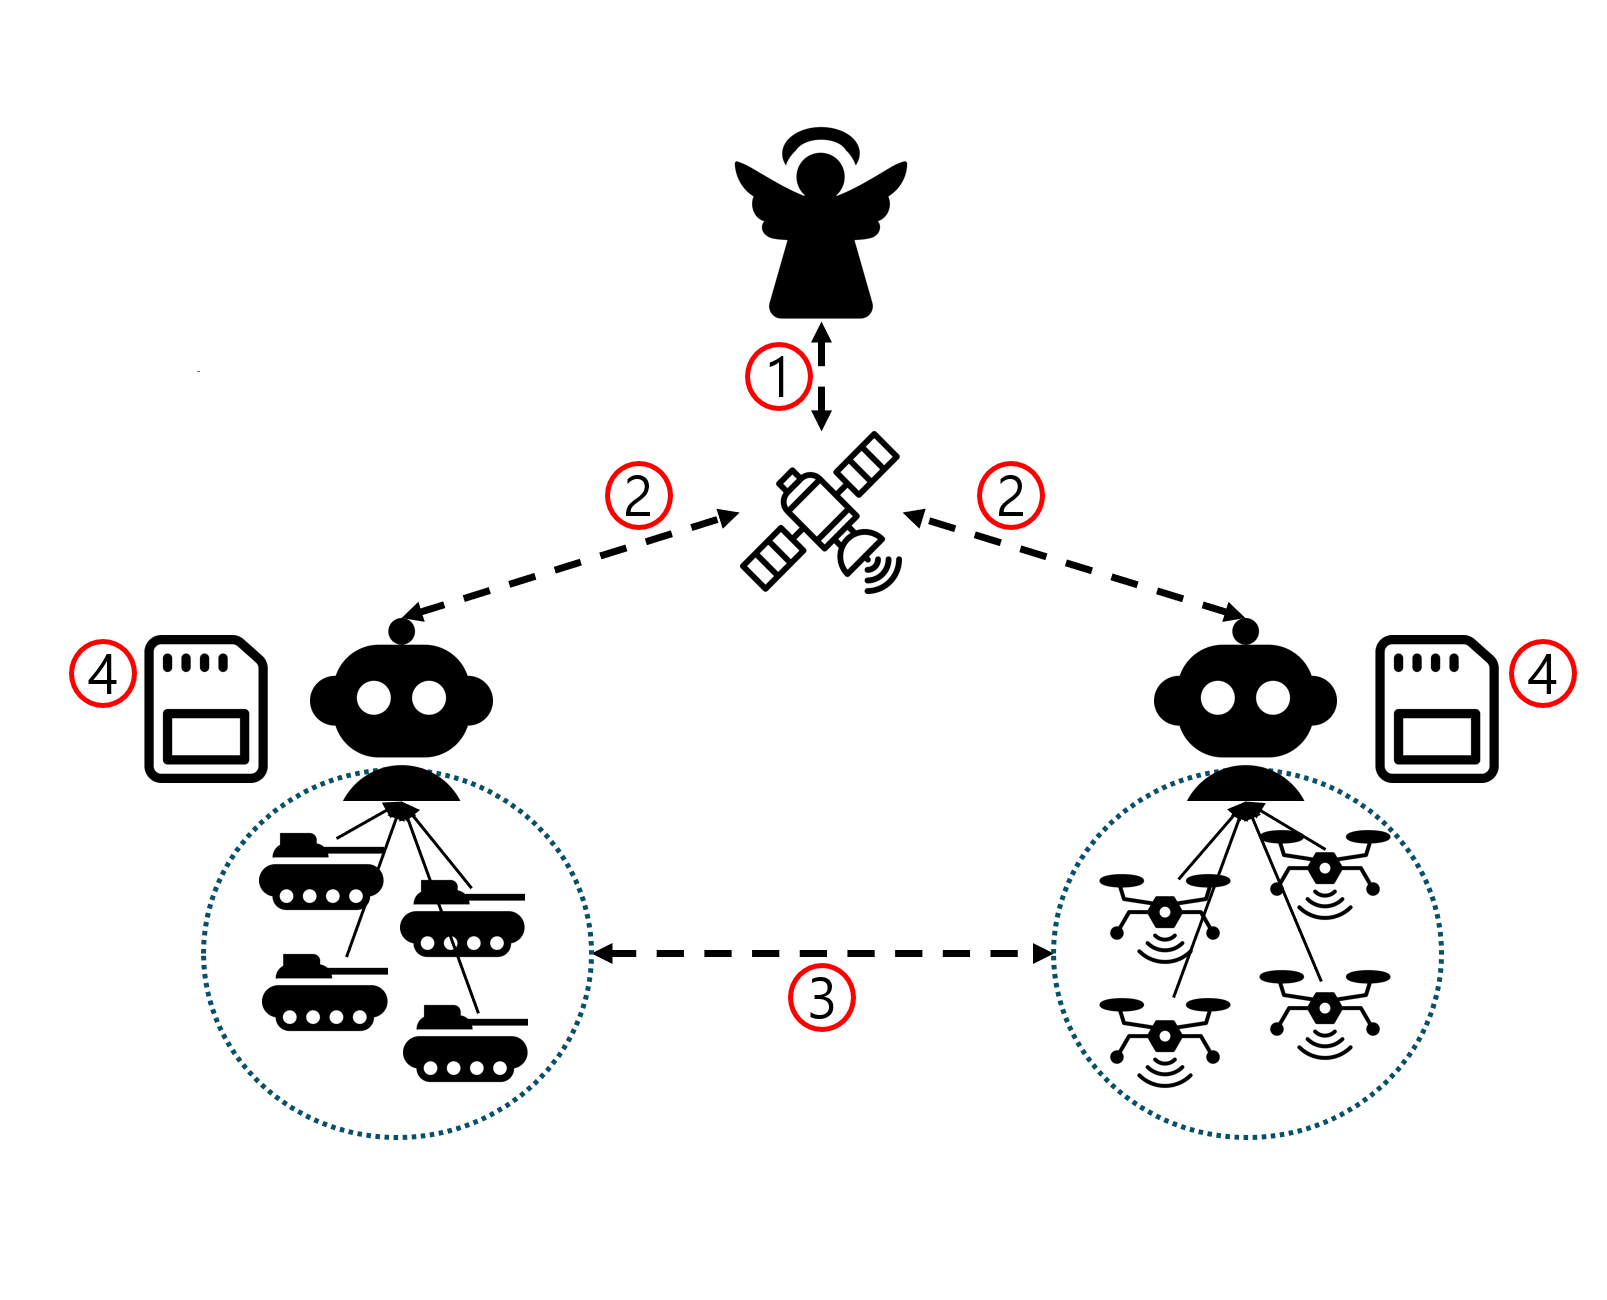
\includegraphics[width=0.85\textwidth]{content/figures/attack_surface.png}
% \caption{다계층 무인체계의 공격 표면(attack surface) 개요. C2/GCS로부터 위성/무선 링크를 거쳐 UGV·UAV로 이어지는 통신 경로와, 각 에이전트가 참조하는 로컬 저장소를 함께 나타낸다. 번호는 본문에서 설명하는 네 가지 공격 지점(①--④)에 대응하며, ①·②는 5장에서 실제로 구현·실측한 MAVLink/링크 계층 공격 지점, ③·④는 7장의 AI 에이전트 아키텍처(RED/BLUE 정보 격리, 지휘관 로컬 상태)와 개념적으로 대응한다.}
% \label{fig:attack_surface}
% \end{figure}

% 표~\ref{tab:attack_defense_overview}는 5~6장에서 상술할 14개 공격(+ADS-B 탐지기 전용 시나리오)과 그 대응 방어를 도메인별로 요약한 것이다. 각 공격은 \texttt{src/attacks/}, 각 방어는 \texttt{src/defenses/} 아래의 실제 파이썬 모듈로 존재한다.

% \begin{table}[t!]
% \centering
% \caption{도메인별 공격/방어 개요 --- 구현 및 실측 완료 (구현: \texttt{src/attacks/}, \texttt{src/defenses/})}
% \label{tab:attack_defense_overview}
% \renewcommand{\arraystretch}{1.2}
% \scriptsize
% \begin{adjustbox}{width=\textwidth}
% \begin{tabular}{p{1.3cm} p{3.4cm} p{3.5cm} p{3.0cm} p{2.6cm}}
% \toprule
% \textbf{도메인} & \textbf{공격} & \textbf{공격 모듈} & \textbf{방어 모듈} & \textbf{예방 티어} \\
% \midrule
% UAV & RC 오버라이드(PITCH ch2) & \texttt{rc\_override.py} & D5 + D6 & [LIVE] BRAKE \\
% UAV & 명령 주입(DO\_SET\_MODE$\to$RTL) & \texttt{command\_injection.py} & D2 + D-SIGN & [SIGN] \\
% UAV & GPS 완만 기만 & \texttt{gps\_spoof.py} & D3 & [LIVE] EKF 소스전환 \\
% UAV & GNSS 재밍/거부 & \texttt{gnss\_jam.py} & D7(GNSS 건전성) & [DETECT-ONLY]+[NATIVE-FS] \\
% UAV & 지자기 스푸핑 & \texttt{sensor\_spoof.py} & D-XCHK & [DETECT-ONLY] \\
% UAV & IMU / 기압 스푸핑 & \texttt{imu\_spoof.py}, \texttt{baro\_spoof.py} & D-IMU, D-BARO & [DETECT-ONLY] \\
% UAV & 미션 / 파라미터 변조 & \texttt{mission\_tamper.py}, \texttt{param\_tamper.py} & D-MISSION, D-PARAM + D-SIGN & [SIGN]+[LIVE-restore] \\
% UAV & ADS-B 유령 항공기 & (하니스 주입) & D-ADSB & [DETECT-ONLY] \\
% \hdashline
% UGV & 조향 채널 오버라이드 & \texttt{rover\_steering.py} & D5 + D6 & [LIVE] HOLD \\
% UGV & 명령 주입 + 이동 중 disarm & \texttt{command\_injection.py} & D2 + D-SIGN & [SIGN] \\
% UGV & GPS 완만 기만 & \texttt{gps\_spoof.py} & D3 & [LIVE] EKF 소스전환 \\
% \hdashline
% 위성/BLOS & 링크 열화(지연/지터/손실) & \texttt{mav\_proxy.py}+\texttt{link\_shaper.py} & D4 & [NATIVE-FS-ready] \\
% 위성/BLOS & DoS 블랙아웃 & \texttt{mav\_proxy.py} & D4 & [NATIVE-FS-ready] \\
% 위성/BLOS & 대역폭 flooding & \texttt{mav\_flood.py} & D4(ingress-rate) & [LIVE] rate-limit \\
% 위성/BLOS & 프레임 재전송(replay) & \texttt{replay.py} & D-REPLAY + D-SIGN & [SIGN] \\
% \bottomrule
% \end{tabular}
% \end{adjustbox}
% \end{table}

% 각 행의 상세 위협 서사·창발 결과·증거 경로는 5장에서, 탐지·차단·복구의 결합 논리와 정직성 티어 태깅은 6장에서, 이 파이프라인을 실제로 구동하는 LLM 기반 RED/BLUE 에이전트 아키텍처는 7장에서 다룬다.

그림~\ref{fig:attack_surface}은 본 연구에서 다루는 다계층 무인체계 공격 표면을 나타낸다. C2/GCS로부터 위성 또는 무선 링크를 거쳐 UGV와 UAV로 이어지는 통신 경로가 핵심 공격면을 구성한다. 또한 각 에이전트가 참조하는 로컬 저장소와 지휘관 상태도 별도의 신뢰 경계로 다룬다.

\begin{figure}[t!]
\centering
% \includegraphics[width=0.85\textwidth]{content/figures/agent_surface.png}
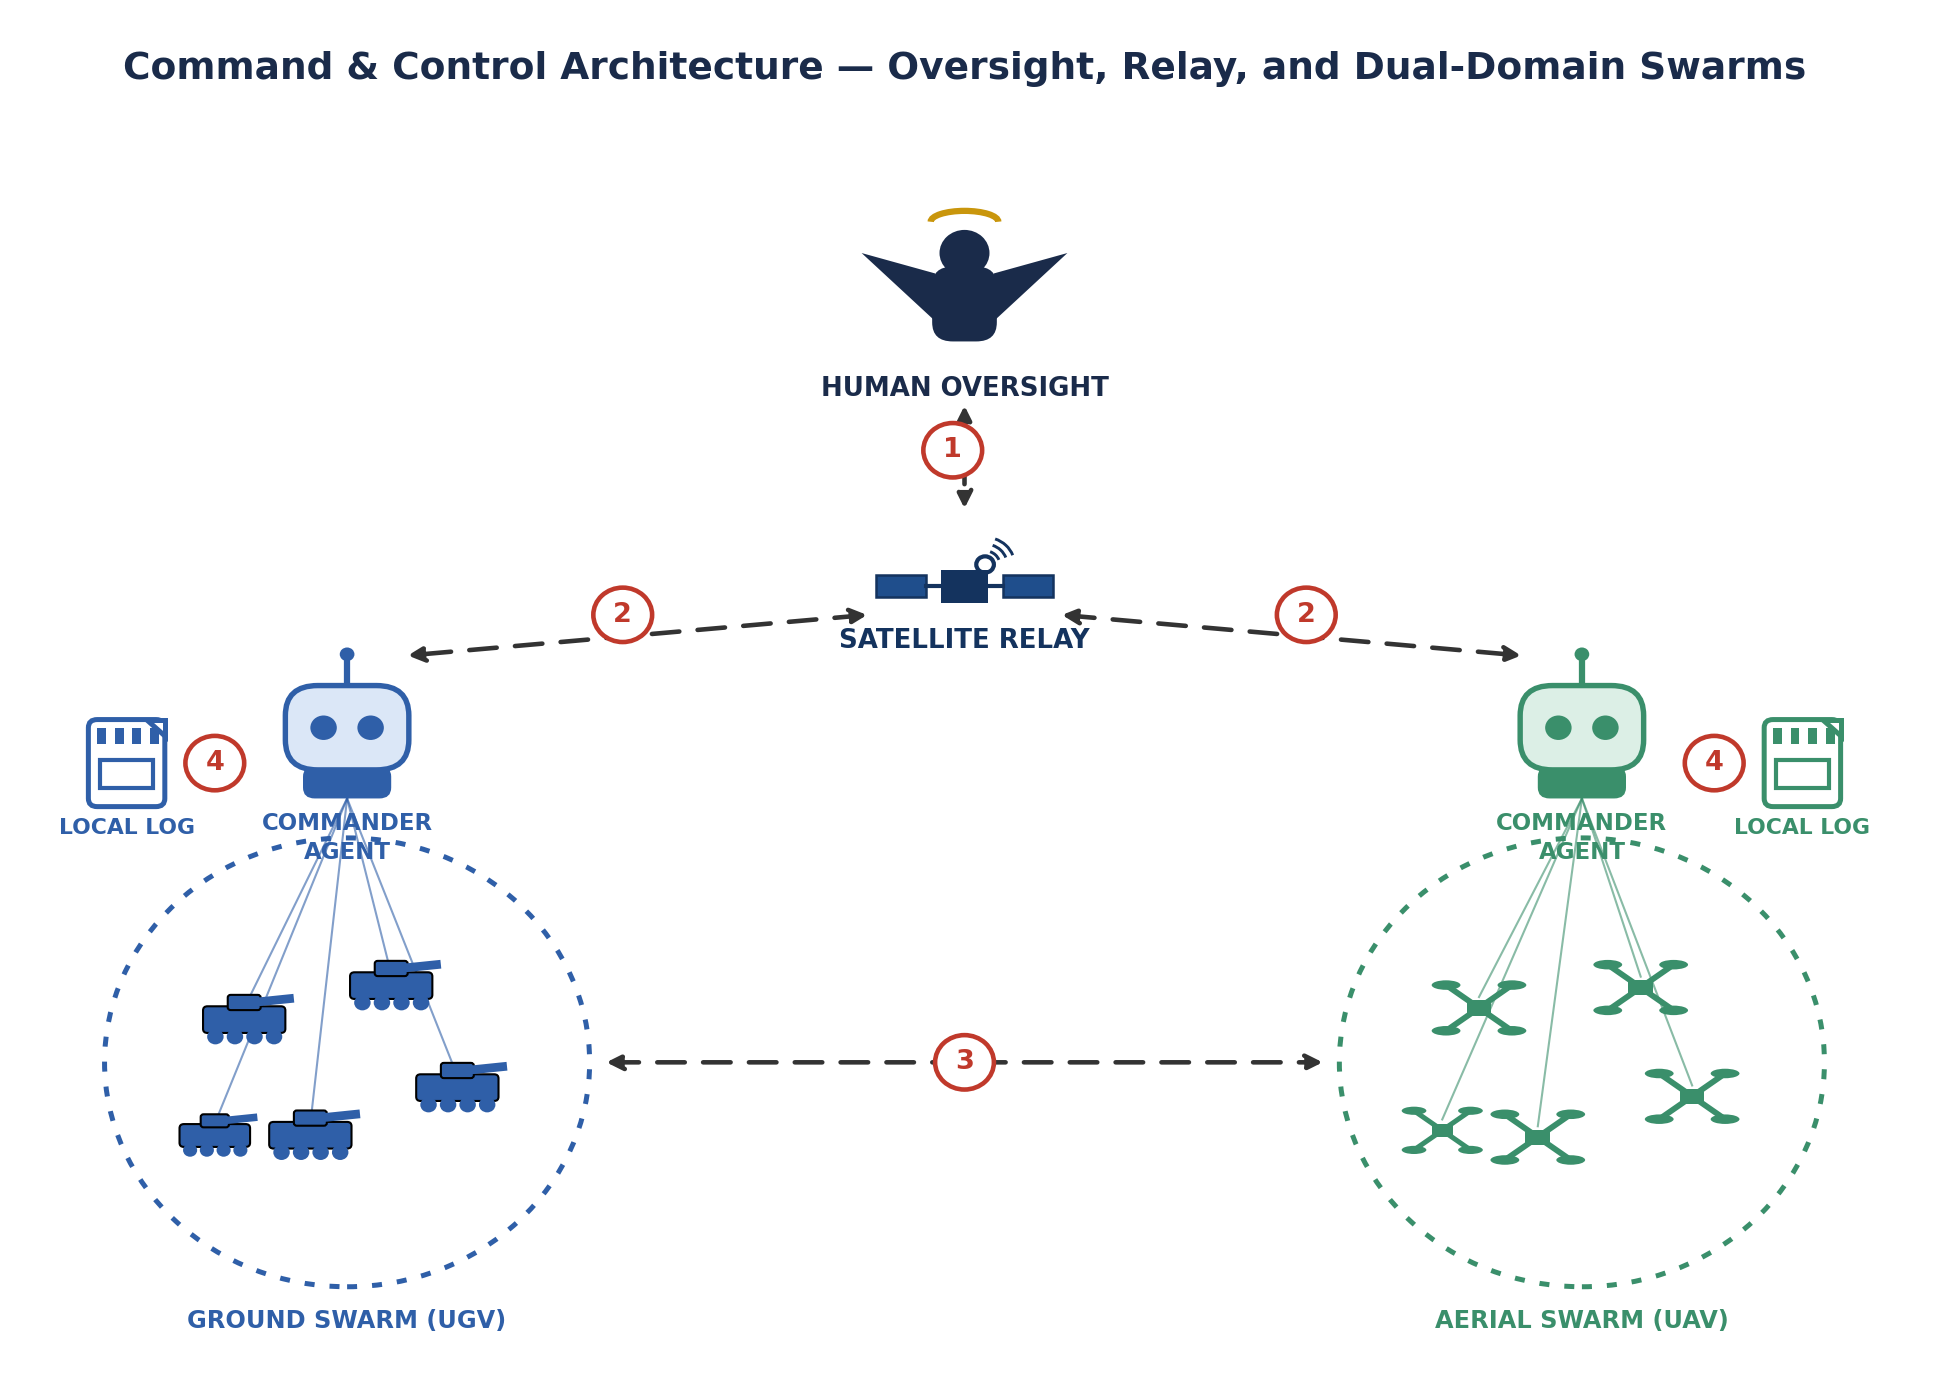
\includegraphics[width=0.75\textwidth]{content/figures/command_control_diagram.png}
\caption{다계층 무인체계의 공격 표면 (Attack surface) 개요. C2/GCS로부터 위성/무선 링크를 거쳐 UGV·UAV로 이어지는 통신 경로와, 각 에이전트가 참조하는 로컬 저장소를 함께 나타낸다. 번호는 본문에서 설명하는 네 가지 공격 지점 (①--④)에 대응한다. ①·②는 5장에서 구현·실측하는 MAVLink/링크 계층 공격 지점이며, ③·④는 7장의 AI 에이전트 아키텍처, RED/BLUE 정보 격리, 지휘관 로컬 상태와 개념적으로 대응한다.}
\label{fig:attack_surface}
\end{figure}

표~\ref{tab:attack_defense_overview}는 5장과 6장에서 상세히 다루는 14개 공격 및 ADS-B 탐지기 전용 시나리오와 그 대응 방어를 도메인별로 요약한다. 각 공격은 \texttt{src/attacks/}, 각 방어는 \texttt{src/defenses/} 아래의 실제 파이썬 모듈로 존재한다.

\begin{table}[t!]
\centering
\caption{도메인별 공격/방어 개요 --- 구현 및 실측 대상}
\label{tab:attack_defense_overview}
\renewcommand{\arraystretch}{1.2}
\scriptsize
\begin{adjustbox}{width=\textwidth}
\begin{tabular}{p{1.3cm} p{3.4cm} p{3.5cm} p{3.0cm} p{2.6cm}}
\toprule
\textbf{도메인} & \textbf{공격} & \textbf{공격 모듈} & \textbf{방어 모듈} & \textbf{예방 티어} \\
\midrule
UAV & RC 오버라이드(PITCH ch2) & \texttt{rc\_override.py} & D5 + D6 & [LIVE] BRAKE \\
UAV & 명령 주입(DO\_SET\_MODE$\to$RTL) & \texttt{command\_injection.py} & D2 + D-SIGN & [SIGN] \\
UAV & GPS 완만 기만 & \texttt{gps\_spoof.py} & D3 & [LIVE] EKF 소스전환 \\
UAV & GNSS 재밍/거부 & \texttt{gnss\_jam.py} & D7 (GNSS 건전성) & [DETECT-ONLY]+[NATIVE-FS] \\
UAV & 지자기 스푸핑 & \texttt{sensor\_spoof.py} & D-XCHK & [DETECT-ONLY] \\
UAV & IMU / 기압 스푸핑 & \texttt{imu\_spoof.py}, \texttt{baro\_spoof.py} & D-IMU, D-BARO & [DETECT-ONLY] \\
UAV & 미션 / 파라미터 변조 & \texttt{mission\_tamper.py}, \texttt{param\_tamper.py} & D-MISSION, D-PARAM + D-SIGN & [SIGN]+[LIVE-restore] \\
UAV & ADS-B 유령 항공기 & 하니스 주입 & D-ADSB & [DETECT-ONLY] \\
\hdashline
UGV & 조향 채널 오버라이드 & \texttt{rover\_steering.py} & D5 + D6 & [LIVE] HOLD \\
UGV & 명령 주입 + 이동 중 disarm & \texttt{command\_injection.py} & D2 + D-SIGN & [SIGN] \\
UGV & GPS 완만 기만 & \texttt{gps\_spoof.py} & D3 & [LIVE] EKF 소스전환 \\
\hdashline
위성/BLOS & 링크 열화 (지연/지터/손실) & \texttt{mav\_proxy.py}+\texttt{link\_shaper.py} & D4 & [NATIVE-FS-ready] \\
위성/BLOS & DoS 블랙아웃 & \texttt{mav\_proxy.py} & D4 & [NATIVE-FS-ready] \\
위성/BLOS & 대역폭 flooding & \texttt{mav\_flood.py} & D4(ingress-rate) & [LIVE] rate-limit \\
위성/BLOS & 프레임 재전송(replay) & \texttt{replay.py} & D-REPLAY + D-SIGN & [SIGN] \\
\bottomrule
\end{tabular}
\end{adjustbox}
\end{table}

각 행의 상세 위협 서사, 창발 결과, 증거 경로는 5장에서 다룬다. 탐지, 차단, 복구의 결합 논리와 정직성 티어 태깅은 6장에서 다룬다. 이 파이프라인을 구동하는 LLM 기반 RED/BLUE 에이전트 아키텍처는 7장에서 다룬다. % 배경지식 및 위협 모델

\section{공격 시나리오}

\subsection{시나리오 구성 원칙}

% 본 절은 4장의 위협 모델 (공격자 능력, 구현 계층)을 바탕으로, UAV·UGV·위성/BLOS 세 도메인에서 실제 운용 맥락 위에 성립하는 \textbf{14개 공격}을 ArduPilot SITL 위에서 구현·실행한 결과를 상술한다. 모든 정량 수치는 \emph{주입량 (injected quantity)}과 \emph{창발적 임무 결과 (emergent mission outcome)}를 명시적으로 분리하며 헤드라인 주입값이 아니라 실제로 기체·임무에 일어난 결과를 기준 수치로 삼는다. 근거는 전부 \texttt{docs/evidence/} 및 \texttt{docs/honest\_effect\_metrics.md}에서만 인용하며, 근거가 없는 항목은 미측정 또는 설계 수준으로 표기한다. 탐지·차단·복구의 상세 설계는 6장으로 이관하고, 본 절에서는 시나리오당 공격 수치만 기술한다.



본 절은 앞선 4장에서 정의한 위협 모델 (공격자의 능력 한계 및 계층별 접근성)을 기반으로, 무인기 (UAV), 무인차량 (UGV), 그리고 위성 및 가시거리 밖 (BLOS, Beyond Line-of-Sight) 데이터링크 등 세 가지 주요 방산 도메인을 전제로 설계한 \textbf{14개의 핵심 공격 시나리오}를 분석한다. 
%
각 공격은 실제 운용 맥락을 고려해 설계하며, 이를 ArduPilot Software-In-The-Loop(SITL) 시뮬레이션 환경에서 직접 구현 및 실행하여 발생한 결과를 바탕으로 상술한다. 
%
특히 모든 시나리오의 정량적 평가 시나리오는 공격자가 물리적으로 주입한 \emph{주입량 (Injected Quantity)}과 이를 통해 시스템 전반에 파생된 \emph{창발적 임무 결과 (Emergent Mission Outcome)}를 명시적으로 분리해 다룬다.  
%
아울러 각 시나리오에 대응하는 탐지, 차단, 복구의 상세 설계 아키텍처는 후속 6장으로 이관하여 심층적으로 다루되, 본 절에서는 공격-방어 맥락의 연결성을 위해 공격 시나리오별로 연계되는 대표적인 방어 기법을 요약식으로 병기한다.


\subsection{UAV 도메인 - ISR/타격/체공 무인기}

UAV 임무는 (a) ISR 감시정찰의 장기 체공 (LOITER), (b) 타격의 AUTO 항로 비행 후 유도, (c) 체공 대기로 나뉘며, 세 프로파일 모두 자율 위치 유지 또는 자율 항로 추종 상태에서 조종사의 실시간 스틱 입력이 없는 구간이 길다는 특징이 있다. 스틱 입력이 0이어야 정상이라는 사실이 오버라이드 주입을 탐지 가능한 불변식으로 전환한다 (4.2절).

\paragraph{\textbf{T-UAV-1 · 단일채널 RC 오버라이드}} ~\\
\textbf{공격 시나리오:} 
% ISR UAV가 30 m LOITER 위치 유지 중, 경로상의 공격자가 PITCH(ch2) 채널 1개만 고정 off-neutral 값으로 위조하고 나머지 7개 채널은 정상 통과시킨다.
감시정찰(ISR) UAV가 30 m 상공에서 위치 유지 임무를 수행하는 도중, 경로상에 위치한 공격자가 피치(PITCH, 채널 2) 신호 단 하나를 위조하고 나머지 채널은 정상 통과시킨 조작 공격이다.
\\
\textbf{실험 결과:} 위치 유지 상태에서 \textbf{수평 이탈이 최대 $\approx$ 65.2 m}까지 발생한다 (임계치 5 m, baseline 0.0 m). 5회 fresh-boot 전체에서 공격에 성공하여 ASR 5/5를 기록한다.\\
% 근거: \texttt{src/attacks/rc\_override.py}; \texttt{docs/evidence/sweep\_UAV\_rc\_override/aggregate.json}. 
% [방어: D5 command-invariant TTD 0.204 s, 0 FP; D-SIGN이 위조 프레임 288개 전량 drop]  
% \paragraph{ \textbf{T-UAV-1 · 단일채널 RC 오버라이드.} }
% ISR UAV가 30 m LOITER 위치 유지 중, 경로상 공격자가 PITCH(ch2) 1개만 위조하고 나머지 7채널을 통과시킨다. 고정 off-neutral PITCH 주입 $\to$ 위치 유지에서 \textbf{수평 이탈 최대 $\approx$ 65.2 m} (임계 5 m, baseline 0.0 m), ASR 5/5(5회 fresh-boot). 
% % 근거: \texttt{src/attacks/rc\_override.py}; \texttt{docs/evidence/sweep\_UAV\_rc\_override/aggregate.json}. 
% % [방어: D5 command-invariant TTD 0.204 s, 0 FP; D-SIGN이 위조 프레임 288개 전량 drop]
\paragraph{\textbf{T-UAV-2 · 위조 명령 주입 (임무 중단)}} ~\\
\textbf{공격 시나리오:} 
% 타격 UAV가 3-WP AUTO 항로 비행을 수행 중인 상황에서, 공격자가 신뢰할 수 있는 시스템 ID (sysid 255)를 사칭하여 단일 \texttt{DO\_SET\_MODE $\to$ RTL} 프레임 1개를 주입한다.
타격 임무를 부여받은 UAV가 3개의 경유점 (WP)을 포함하는 자율 (AUTO) 항로를 비행하던 도중, 신뢰할 수 있는 시스템 ID(255)를 사칭한 위장 \texttt{DO\_SET\_MODE $\to$ RTL(Return-To-Launch)} 프레임을 단 1회 주입하는 시나리오다.
\\
\textbf{실험 결과:} 최종 비행 모드가 RTL로 강제 전환되어 기체가 귀환하며, 3개의 웨이포인트 중 \textbf{2개의 WP에 미도달}하며, 단 1프레임의 주입만으로 전체 임무가 무력화된다.\\
% 근거: \texttt{src/attacks/command\_injection.py}; \texttt{docs/evidence/gap\_cmd\_injection\_ids/}. 클래스 차단 증명: \texttt{docs/evidence/gap2\_mavlink\_signing/}(ASR 1.0$\to$0.0). [방어: D-SIGN = prevention]
% \paragraph{\textbf{T-UAV-2 · 위조 명령 주입 (임무 중단).} }
% 타격 UAV가 3-WP AUTO 항로 비행 중, 신뢰 sysid(255)를 사칭한 단일 \texttt{DO\_SET\_MODE $\to$ RTL} 프레임 1개가 주입된다. 결과적으로 \texttt{final\_mode} RTL, 3-WP 중 \textbf{2 WP 미도달}, 기체 귀환을 시키며 단 1프레임이 전 임무를 무력화한다. 
% 근거: \texttt{src/attacks/command\_injection.py}; \texttt{docs/evidence/gap\_cmd\_injection\_ids/}. 클래스 차단 증명: \texttt{docs/evidence/gap2\_mavlink\_signing/}(ASR 1.0$\to$0.0). [방어: D-SIGN = prevention]
\paragraph{\textbf{T-UAV-3 · GPS 완만 기만 (항법 의존적 창발)}} ~\\
\textbf{공격 시나리오:} UAV가 정지 체공 또는 3-WP AUTO 항로 비행을 수행 중인 상황에서, 공격자가 위치 추정치를 점진적으로 왜곡하는 40 m 저속 램프 (Ramp) 기만 신호를 주입한다.\\
\textbf{실험 결과:} 운용 모드에 따라 결과가 극명하게 갈린다. 
% 정지 체공 중에는 EKF innovation 게이팅이 완전 저항하여 \textbf{실제 이탈이 0.009 m}에 그치나, 3-WP AUTO 항로에서는 동일 램프 주입 시 \textbf{실제 crosstrack 최대 18.31 m} (clean baseline 0.83 m)의 회랑 이탈 및 웨이포인트 미도달 (진짜 miss 8.99 m)이 발생한다. 
기체가 \textbf{단순 정지 체공} 상태일 때는 외부 조작 신호가 주입되어도 확장 칼만 필터 (EKF)의 이노베이션 게이팅 기능이 완전히 이를 거부해, 결과론적 \textbf{이탈 거리는 0.009 m에 불과}하다. 반면, 기체가 \textbf{항로 보정이 지속해서 가해지는 자율 비행} 상태일 경우에는 동일한 공격 램프가 임무 항적을 크게 왜곡해 \textbf{최대 18.31 m에 달하는 측면 이탈 (Crosstrack Error)}을 유발하며, 이는 목표 경유지의 도달 실패로 이어진다.
탐지 후에도 자율 페일세이프가 즉각 개입하지 않아 오염된 트랙을 그대로 비행하는 한계를 보인다.\\
% 근거: \texttt{src/attacks/gps\_spoof.py}; \texttt{docs/evidence/gap\_gps\_spoof\_d3/}. [정직 경계: D3 EKF-innovation 탐지는 TTD 0.81 s, 0 FP로 빠르지만 탐지 $\neq$ 자동 대응. 방어: D3, [LIVE] EKF 소스전환]
% \paragraph{\textbf{T-UAV-3 · GPS 완만 기만 (항법 의존적 창발).} }
% 40 m 저속 램프 주입 시 운용 모드에 따라 결과가 극명하게 갈린다. 정지 체공(LOITER) 중에는 EKF innovation 게이팅이 온전히 방어하여 \textbf{실제 이탈이 0.009 m}에 그치나, 3-WP AUTO 항로 비행 중에는 동일 기만에 의해 \textbf{최대 18.31 m의 crosstrack 이탈} (baseline 0.83 m)이 발생하며 회랑 이탈 및 WP 미도달(오차 8.99 m)을 초래한다. 탐지 이후에도 자율 페일세이프가 즉각 개입하지 않아 오염된 경로를 그대로 비행하는 한계가 관찰된다.
\paragraph{\textbf{T-UAV-4 · GNSS 재밍 및 거부 (항법 소스 상실)}} ~\\
\textbf{공격 시나리오:} 
% GPS 의존 AUTO 모드로 비행 중인 UAV 반경에 공격자가 광대역 재머를 가동하여 항법 신호를 완전히 거부시킨다 (\texttt{SIM\_GPS1\_ENABLE=0 + NUMSATS=0}).
위성항법 의존도가 매우 높은 자율 비행 상태에서 공격자의 광대역 재머가 가동하는 시나리오(\texttt{SIM\_GPS1\_ENABLE=0 + NUMSATS=0})다.
\\
%
%
\textbf{실험 결과:} 
% \texttt{fix\_type}이 6에서 1로 $\sim$0.4 s 만에 붕괴한다. EKF가 관성으로 $\sim$8 s 동안 추측항법(dead-reckon)을 수행하며 이전 추정치로 AUTO 임무를 그대로 비행하나, 이후 페일세이프가 래치되어 \textbf{AUTO $\to$ LAND로 강제 전환} (8.19 s)되며 임무가 중단 (WP4 미도달)된다. 내장 재밍 모델 (\texttt{SIM\_GPS1\_JAM=1}) 검증에서도 45 s 동안 Fix 유형이 92회 전이하는 `불안정 열화 후 완전 상실' 패턴 하에 네이티브 LAND가 4.88 s에 발동함을 확인한다. 광대역 거부 특성상 정상 소스로의 전환은 불가능하며 detect-only가 정직한 한계다.
위성항법 의존도가 매우 높은 자율 비행 상태에서 공격자의 광대역 재머가 가동하는 시나리오(\texttt{SIM\_GPS1\_ENABLE=0 + NUMSATS=0})다. 항법 위성 신호 유형 (Fix type) 붕괴는 약 0.4초 만에 촉발되지만, 즉시 기체가 추락하는 것은 아니다. 기체의 EKF 모듈이 내부 관성 센서를 바탕으로 약 8초가량 추측 항법 (Dead-Reckoning)을 시도하며 낡은 위치 추정치에 의존해 기존 경로를 따라 그대로 비행한다. 이후 비로소 항법 또는 EKF의 페일세이프가 발동해 자율 비행 모드에서 즉각 강제 착륙 모드로 래치 (Latch)되며 임무가 중단된다.
\\
% 근거: \texttt{src/attacks/gnss\_jam.py}; \texttt{docs/evidence/push\_gnss\_jam\_emergent/}, \texttt{enh\_n5\_gnss\_imu\_baro/}, \texttt{enh\_gnss\_jam\_realistic/}. [방어: D7이 fix 붕괴를 0.61 s에 탐지하여 네이티브 LAND보다 7.58 s 선행 경보하나 복구는 ArduPilot 자체 EKF 페일세이프인 [DETECT-ONLY]+[NATIVE-FS] 한계]
% \paragraph{\textbf{T-UAV-4 · GNSS 재밍 및 거부 (항법 소스 상실).} }
% GPS에 의존하는 AUTO 모드 중 광대역 재머 (\texttt{SIM\_GPS1\_ENABLE=0 + NUMSATS=0})가 진입할 경우, $\sim$0.4 s 만에 Fix가 붕괴(6$\to$1)한다. EKF는 관성 기반으로 $\sim$8 s간 추측항법 (dead-reckon)을 유지하나, 이후 페일세이프가 래치되어 \textbf{AUTO에서 LAND 모드로 강제 전환} (8.19 s)되며 임무가 중단된다. 내장 재밍 모델(\texttt{SIM\_GPS1\_JAM=1}) 교차 검증에서도 45 s간 92회의 Fix 전이가 발생하는 '불안정 열화 후 상실' 패턴이 확인되었다. 광대역 거부 특성상 안전한 소스로의 전환은 불가하며, 네이티브 EKF 페일세이프에 의존해야 한다.
% \textbf{T-UAV-4 · GNSS 재밍/거부(항법 소스 상실).} GPS 의존 AUTO 중 광대역 재머가 진입한다(\texttt{SIM\_GPS1\_ENABLE=0 + NUMSATS=0}). fix\_type 6$\to$1로 $\sim$0.4 s 만에 붕괴하나, EKF가 관성으로 $\sim$8 s 추측항법(dead-reckon)하며 낡은 추정치로 AUTO 임무를 그대로 비행한 뒤 나브/EKF 페일세이프가 래치돼 \textbf{AUTO$\to$LAND로 강제}된다(8.19 s, n=2; n=5 rigor 상향 시 8.13 s, std 0.08, 모드전환 100\%). 임무는 완료되지 않는다(WP4 미도달). \textbf{정직 경계:} D7이 fix 붕괴를 0.61 s에 탐지해 네이티브 LAND보다 7.58 s 선행 경보하나, 광대역 재머는 모든 GNSS를 거부하므로 건강한 GPS2로의 소스전환은 불가능하다 --- \textbf{detect-only가 정직한 한계}이고 복구는 ArduPilot 자체 EKF 페일세이프다. 근거: \texttt{src/attacks/gnss\_jam.py}; \texttt{docs/evidence/push\_gnss\_jam\_emergent/}, \texttt{enh\_n5\_gnss\_imu\_baro/}. [방어: D7, [DETECT-ONLY]+[NATIVE-FS]] \textbf{현실성 검증(추가 실측):} 위 킬스위치 모델과 별도로 ArduPilot 내장 재밍 모델(\texttt{SIM\_GPS1\_JAM=1})로도 재검증하였다 --- 위성 수·속도·위치가 흔들리며 45 s 동안 fix 유형이 92회 전이하는 현실적 "불안정 열화 후 완전 상실" 패턴이 나타나며, 이 조건에서도 D7은 0.3 s에 포착(기준선 오탐 0)하고 네이티브 EKF 페일세이프 LAND는 4.88 s에 발동한다(10.3절, 근거: \texttt{docs/evidence/enh\_gnss\_jam\_realistic/}).
\paragraph{\textbf{T-UAV-5 · 지자기 (나침반) 기만}} ~\\
\textbf{공격 시나리오:} 공격자가 나침반 센서에 오프셋 램프 (\texttt{SIM\_MAG1\_OFS})를 주입하여 raw 나침반 heading 오차를 최대 104.44°까지 발생시킨다.\\
\textbf{실험 결과:} 
% 나침반 교차검증 시스템이 이상을 탐지하되 무력화하지 못하며, \textbf{EKF 융합 yaw 오차가 최대 83.42°까지 오염}된다. 센서 다중화 검증만으로는 융합 알고리즘의 오염을 완전히 방어하지 못하는 정직한 detect-only의 한계를 보인다.
공격 주입 시 센서 단의 가공되지 않은 방향 수치 오차가 104.44°까지 인가되며, 이는 EKF 융합 단계를 거치더라도 실질적 기수(Yaw) 오차를 83.42°까지 크게 오염시킨다. 나침반 교차 검증 메커니즘을 통해 탐지는 가능하나 융합 값을 본질적으로 무력화하지는 못한다.
\\
%
% 근거: \texttt{src/attacks/sensor\_spoof.py}; \texttt{docs/evidence/gap2\_sensor\_spoof/}. [방어: D-XCHK TTD 0.61 s, 0 FP - mag 단독은 정직한 detect-only]
% \textbf{T-UAV-5 · 지자기(나침반) 기만.} \texttt{SIM\_MAG1\_OFS} 램프 --- raw 나침반 heading 오차 최대 \textbf{104.44°} 주입 시 \textbf{EKF 융합 yaw 오차가 최대 83.42°까지 오염}되어, 나침반 교차검증은 탐지는 하되 무력화하지 못한다. 근거: \texttt{src/attacks/sensor\_spoof.py}; \texttt{docs/evidence/gap2\_sensor\_spoof/}. [방어: D-XCHK TTD 0.61 s, 0 FP --- mag 단독은 \textbf{정직한 detect-only}]
\paragraph{\textbf{T-UAV-6 · IMU 및 기압 센서 다중화 기만}} ~\\
\textbf{공격 시나리오:} 센서 리던던시 (Redundancy) 구조를 무력화하기 위해, 공격자가 가용 리던던시 전체를 동시에 같은 방향으로 기만하여 투표 (Out-vote) 메커니즘을 우회한다.\\
\textbf{실험 결과:}
% 1) \textbf{IMU 바이어스 (n=3):} 가속/자이로 바이어스 램프 주입 시 페일오버할 깨끗한 관성 소스가 없어 \textbf{EKF 융합 자세가 진값 대비 평균 47° (피크 58°) 오염}되고, 고도 손실 최대 37.2 m, ASR 1.0을 기록한다.\\
% 2) \textbf{기압 스푸핑 (n=3, 성공 2/3):} 두 기압계 모두에 18 m 오프셋 램프 주입 시, 기압이 EKF의 1차 수직 소스이기 때문에 \textbf{실제 물리 강하 최대 $\sim$19.17 m (평균 10.06 m)}로 주입량과 1:1의 창발 결과가 유발된다.\\
고의적인 센서 램프를 주입 시, 융합 자세는 실제 지형값 대비 평균 47° 편차를 유발하고 고도는 최대 37.2 m 가량 손실된다. 공존하는 백업 IMU 체제 전체가 오염되므로, 페일오버를 수행할 대안 센서 자체가 사라진다. 더욱 직관적인 사례로 두 기압계에 18 m 수준의 기압 변위 오프셋 램프를 동시에 주입하면, 기압은 수직 항법 보조의 1차 주요 데이터 소스이기 때문에 \textbf{기체는 정확히 약 19.17 m 수준의 고도 강하를 물리적으로 실행}한다.
%
% 근거: \texttt{src/attacks/imu\_spoof.py}, \texttt{baro\_spoof.py}; \texttt{docs/evidence/push\_imu\_spoof\_emergent/}, \texttt{push\_baro\_spoof\_emergent/}. [방어: 둘 다 detect-only, D-IMU TTD 1.57 s, D-BARO TTD 2.7 s, 0 FP]
% \textbf{T-UAV-6 · IMU / 기압 센서 기만.} 센서 다중화가 있어도 모든 리던던시를 동시에 같은 방향으로 밀면 out-vote가 무력화된다. \textbf{IMU 바이어스(n=3):} 가속/자이로 바이어스 램프 $\to$ EKF 융합 자세가 진값 대비 평균 \textbf{47°}(피크 58°) 오염, 고도 손실 최대 37.2 m, ASR 1.0 --- 공존 IMU를 모두 밀었으므로 페일오버할 오염되지 않은 관성 소스가 없다(detect-only, D-IMU TTD 1.57 s, 0 FP). \textbf{기압 스푸핑(n=3, 성공 2/3):} 두 기압계 모두에 18 m 오프셋 램프 $\to$ \textbf{실제 물리 강하 최대 $\sim$19.17 m(평균 10.06 m), 주입량과 $\sim$1:1} --- 기압은 EKF의 1차 수직 소스라서 주입량 $\approx$ 창발 결과다(GPS-호버의 정반대). D-BARO TTD 2.7 s, 0 FP. 근거: \texttt{src/attacks/imu\_spoof.py}, \texttt{baro\_spoof.py}; \texttt{docs/evidence/push\_imu\_spoof\_emergent/}, \texttt{push\_baro\_spoof\_emergent/}. [방어: 둘 다 detect-only]
\paragraph{\textbf{T-UAV-7 · 미션 및 파라미터 변조}} ~\\
\textbf{공격 시나리오:} 
MAVLink 미션 프로토콜 (\texttt{MISSION\_WRITE\_PARTIAL\_LIST})과 파라미터 설정 (\texttt{PARAM\_SET})의 v1 무인증 취약점을 악용하여 악성 명령을 주입한다.\\
\textbf{실험 결과:}
MAVLink 통신은 미션 프로토콜과 파라미터 변수 변경 구간을 인증 절차 없이 수용한다. 공격자가 임무 스케줄(Partial-List)을 조작해 기체의 두 번째 경유점 (Way-Point) 위치를 기지정된 150 m 범위의 지오펜스 (Geo-Fence)를 한참 벗어난 180 m 지점으로 재구축한다. 유입된 인자는 기체의 자율 비행 체계를 가상 남쪽 지점인 심연으로 끌어들여 비행 88.6초 시점에 지오펜스 침범 오작동을 유발한다. 나아가, 강제 보호 규정을 담당하는 제어 환경설정 (\texttt{PARAM\_SET})에 접근해 무선 채널 상실 시 자동 발동하는 귀환 절차 스위치를 인위적으로 차단한다(\texttt{FS\_THR\_ENABLE $\to$ 0}). 보호 RTL(Return-To-Launch) 절차는 즉각적으로 무력화되어 링크가 끊어져도 기체는 위험 지대에 한없이 체공(LOITER)하게 된다.
%
% 근거: \texttt{src/attacks/mission\_tamper.py}, \texttt{param\_tamper.py}; \texttt{docs/evidence/push\_mission\_param\_emergent/}. [방어: D-SIGN이 클래스 차단, D-MISSION(0.175 s 탐지) 및 D-PARAM(1.34 s 탐지 및 재확정 복구, ASR 1.0$\to$0.0)]
% \textbf{T-UAV-7 · 미션/파라미터 변조.} MAVLink 미션 프로토콜(\texttt{MISSION\_WRITE\_PARTIAL\_LIST})과 \texttt{PARAM\_SET}은 v1 무인증이다. \textbf{미션 리라우트:} 위조 partial-list로 seq2를 홈 남쪽 180 m(150 m 정책 지오펜스 밖)로 재작성 $\to$ AUTO 트랙이 실제로 남쪽 $\sim$180 m까지 끌려가 88.6 s에 지오펜스 침범. D-MISSION이 무단 쓰기·plan-hash 변경을 0.175 s에 탐지, 오탐 0. \textbf{파라미터 변조 $\to$ 페일세이프 억제:} \texttt{PARAM\_SET}로 \texttt{FS\_THR\_ENABLE 1$\to$0} --- 이후 RC-링크 상실 시 보호 RTL이 더 이상 발동하지 못한다(baseline 1.15 s RTL vs 공격 시 LOITER 유지). D-PARAM이 1.34 s에 탐지·복구(재확정 $\to$ 억제 ASR 1.0$\to$0.0). 근거: \texttt{src/attacks/mission\_tamper.py}, \texttt{param\_tamper.py}; \texttt{docs/evidence/push\_mission\_param\_emergent/}. [방어: D-SIGN이 클래스 차단, D-MISSION/D-PARAM이 탐지+복구]
\paragraph{\textbf{T-UAV-8 · ADS-B 유령 항공기 기만 (충돌 회피 악용)}} ~\\
\textbf{공격 시나리오:} ISR UAV가 LOITER 중 ADS-B 충돌회피 (\texttt{AVD\_ENABLE=1})가 활성화된 상태에서, 공격자가 무인증 \texttt{ADSB\_VEHICLE} 프레임을 주입하여 399.6 m 이내로 진입하는 가상의 유령 항공기를 생성한다.\\
\textbf{실험 결과:} 
% 시스템이 유령 항공기를 실제 위협으로 오인하여 \textbf{0.49 s 만에 LOITER $\to$ AVOID\_ADSB 모드로 전환되고, 측방으로 $\sim$320 m 강제 회피} 후 복귀함으로써 원래의 임무 위치를 이탈한다. 저속 직진 접근(Ramp-in) 유령기 주입 시 기존 규칙(R1-R3)이 모두 우회됨을 포착하여 지속-접근 규칙 \textbf{R4(sustained-inbound)}를 추가 기술(\texttt{adsb\_xcheck.py})하였으며, 105 s (range 1238.6 m)에 포착 성공한다. 다만 R4는 CPA를 보지 않고 순접근만 판단하므로 정당한 수렴 교통에 오탐할 수 있는 정직한 잔여 한계 (CPA·방위율 게이트 필요)가 존재한다.
공격자가 생성한 허상의 비행체 항적 정보를 바탕으로 충돌 회피 방어 모듈 (\texttt{AVD\_ENABLE})이 자동 대응을 개시해, 단 0.49초 만에 320 m 수준의 우발적 측방 회피 기동을 야기한다. 허상과 충돌하지 않으려는 자동 반사적 통제 로직 자체가, 기체를 의도된 주요 운용 지점에서 손쉽게 우회 및 배제하는 강력한 공격자의 지렛대 역할로 작용한다.
% 근거: \texttt{docs/evidence/surf\_adsb\_spoof/}, \texttt{surf\_adsb\_rampin/}. [방어: D-ADSB 탐지(detect-only)]
% \textbf{T-UAV-8 · ADS-B 유령 항공기 기만.} ISR UAV가 LOITER 중 ADS-B-in 충돌회피(\texttt{AVD\_ENABLE=1}) 활성. 무인증 \texttt{ADSB\_VEHICLE} 프레임 주입 $\to$ 유령 항공기(399.6 m inbound) 생성 $\to$ \textbf{LOITER$\to$AVOID\_ADSB 0.49 s 반응, $\sim$320 m 측방 회피} 후 LOITER 복귀 --- 유령이므로 진짜 위협은 없으나 기체가 임무 위치를 이탈한다(네이티브 회피 자체가 공격자의 지렛대). \textbf{특수 지위:} 별도 \texttt{src/attacks} 모듈이 아니라 증거 하니스 주입이며, 탐지기 D-ADSB만 shipped된다. 단일 계측런이며 저속·플로시블 램프-인은 회피 가능하다. 근거: \texttt{docs/evidence/surf\_adsb\_spoof/}. [방어: detect-only] \textbf{gap 실측 및 closing(추가 실측):} 위에서 지적한 회피 가능성을 실제로 검증하였다 --- 첫 관측 2497 m에서 12 m/s로 직진 접근하는 저속 유령기를 주입하면 R1--R3 규칙을 모두 회피한다(경보 0/205건). 이를 닫기 위해 지속-접근 규칙 \textbf{R4(sustained-inbound)}를 \texttt{adsb\_xcheck.py}에 추가하여, 근접 밖에서 획득되었으나 지속적으로 순접근하는 항적을 105 s(range 1238.6 m)에 포착하면서, 단순 통과 항적에는 오탐 0을 유지한다. 다만 R4 자체를 사후에 red-team한 결과 최근접점(CPA)을 보지 않고 순접근만 판단하므로 정당한 수렴 교통(예: 500 m 이격의 실제 착륙 접근기)에는 오탐할 수 있음을 확인하였다 --- CPA·방위율 게이트가 필요한 정직한 잔여 한계다(10.3절, 근거: \texttt{docs/evidence/surf\_adsb\_rampin/}).
\subsection{UGV 도메인 --- 자율 호송/군수/정찰 무인차량}
% UGV는 GPS-denied 도심·지하·터널·건물 내부에 더 자주·오래 노출되며, 지상 근접이라 근거리 개입 위험도 크다. 실측 통찰에 따르면 (i) 자율 (AUTO) 자체가 작동기 격리 계층이다 (사전계획 미션 중엔 수동 스틱 입력이 없어야 정상); (ii) 이동 중 모터 차단(in-motion disarm)에 대해 rover 펌웨어는 copter와 달리 방어하지 않는다 (플랫폼 특수 위험).
% 지상 운용 로버 (Rover) 기체로 대변되는 UGV 도메인은 UAV와 확연히 다른 지상 운용 특수성을 갖는다. 도심, 터널, 건물 내부 등 빈번한 GPS 단절 구역 운용 환경에 노출되며 적대자나 외부 기기와 물리적으로 근접해 조우하기 쉽다. 특히, 로버 펌웨어 상에서는 주행 중 원격 차단 명령 (In-motion disarm)을 여과 없이 수용해 구동계를 완전히 중지시켜 버리는 플랫폼 측면의 특이 취약점이 큰 위협으로 작용한다.

지상 운용 로버 (Rover) 기체로 대변되는 UGV 도메인은 UAV와 확연히 구별되는 지상 운용의 특수성을 지닌다. 도심, 터널, 건물 내부 등 GNSS 거부 (Denial) 및 단절 환경에 빈번하게 노출되며, 적대자 또는 외부 기기와 물리적으로 근접하여 조우할 가능성이 높다. 특히, 로버 펌웨어는 주행 중 원격 차단 명령 (In-motion disarm)을 여과 없이 수용하여 구동계를 완전히 중지시키는 플랫폼 고유의 취약점을 내포하고 있어 큰 위협으로 작용한다.

\paragraph{\textbf{T-UGV-1 · 조향 채널 오버라이드}} ~\\
\textbf{공격 시나리오:} ArduRover가 직선 경로를 주행 중인 상황에서, 공격자가 조향 제어 채널인 STEER (ch1) 단 하나의 채널만을 변조하여 고정된 위조 값을 주입하고 나머지 채널은 정상 통과시킨다.\\
%\textbf{실험 결과:} 기체의 \textbf{heading (방위각) 이탈이 최대 $\approx$ 179.7--180°} 발생하여 사실상 완전 반전 주행을 유도하며, 이로 인해 \textbf{최대 $\approx$ 27.3 m의 경로 이탈} (임계치 30° 또는 5 m, baseline crosstrack $\approx$ 0.9 m)을 초래하며, 5회 시도 모두 성공하여 ASR 5/5를 기록한다.\\
\textbf{실험 결과:} 기체의 방위각 (Heading) 이탈이 최대 약 179.7--180° 발생하여 사실상 완전한 반전 주행이 유도된다. 이로 인해 창발적 임무 결과로서 최대 27.3 m의 경로 이탈 (임계치 30° 또는 5 m, 대조군 교차항적오차 약 0.9 m)이 초래되며, 5회 시도 모두 성공하여 공격성공률 (ASR) 1.0 (5/5)을 기록한다.\\

% 근거: \texttt{src/attacks/rover\_steering.py}; \texttt{docs/evidence/sweep\_UGV\_steering/}. 
% [방어: D5 탐지 TTD 0.204 s --- 실운용 시스템에서는 실제 flight-mode 신호에 기반한 불변식 gating 방어 필요]

% \textbf{T-UGV-1 · 조향 채널 오버라이드.} ArduRover 직선 경로 주행 중 STEER(ch1) 1채널만 위조 $\to$ \textbf{heading 이탈 최대 $\approx$179.7--180°}(사실상 완전 반전), \textbf{경로 이탈 최대 $\approx$27.3 m}(임계 30°/5 m, baseline crosstrack $\approx$0.9 m), ASR 5/5. 근거: \texttt{src/attacks/rover\_steering.py}; \texttt{docs/evidence/sweep\_UGV\_steering/}. [방어: D5 TTD 0.204 s --- production은 실제 flight-mode 신호에 불변식 gating 필요]

\paragraph{\textbf{T-UGV-2 · 명령 주입 및 주행 중 모터 차단}} ~\\
\textbf{공격 시나리오:} Rover가 AUTO 모드로 설정된 경로를 실제 추종 및 주행 중인 상황에서, 공격자가 악의적으로 위조된 HOLD 또는 RTL 모드 전환 명령 (\texttt{DO\_SET\_MODE})과 함께 이동 중 시동 잠금 (\texttt{DISARM}) 프레임을 주입한다.\\
%\textbf{실험 결과:} 강제적인 HOLD 및 RTL 모드가 수용될 뿐만 아니라, 기체가 \textbf{1.05 m/s의 속도로 주행 중임에도 불구하고 disarm 명령이 최종 수용되어 모터 동력이 주행 중 완전히 차단}된다. 이는 드론 (Copter) 플랫폼이 공중 disarm 명령을 거절하는 보안 기제를 갖춘 것과 대조되는 지상 로버 플랫폼 고유의 특수 취약점이다.\\
\textbf{실험 결과:} 강제적인 HOLD 및 RTL 모드 전환이 수용될 뿐만 아니라, 기체가 1.05 m/s의 속도로 주행 중임에도 불구하고 시동 잠금 명령이 최종 수용되어 모터 동력이 완전히 차단된다. 이는 공중 차단 명령을 거부하는 보안 기제를 갖춘 드론 플랫폼과 대조되는 지상 로버 플랫폼 고유의 특수 취약점이다.\\
% 근거: \texttt{src/attacks/command\_injection.py}; \texttt{docs/evidence/gap2\_ugv\_roundout/}. 
% [방어: R1/R2 명령 기반 IDS TTD 0.42--1.22 s 및 D-SIGN 방어]
% \textbf{T-UGV-2 · 실제 AUTO 미션 중 명령 주입 + 이동 중 모터 차단.} rover가 실제 AUTO 경로추종 중, 위조 HOLD/RTL \texttt{DO\_SET\_MODE} + 이동 중 \texttt{DISARM}. HOLD·RTL 적용됨; \textbf{1.05 m/s 주행 중 disarm이 수용되어 모터가 이동 중 절단}된다 --- copter는 공중 disarm을 거부하나 rover는 수용하는 플랫폼 특수 취약이다. 근거: \texttt{src/attacks/command\_injection.py}; \texttt{docs/evidence/gap2\_ugv\_roundout/}. [방어: R1/R2 명령 IDS TTD 0.42--1.22 s + D-SIGN]
\paragraph{\textbf{T-UGV-3 · GPS 완만 기만 (지상 기체 선형 이탈)}} ~\\
\textbf{공격 시나리오:} Rover가 AUTO 모드로 주행 중인 상황에서, 공격자가 위성 항법 (GPS) 신호에 35 m 오차의 램프 (Ramp) 기만 신호를 점진적으로 주입한다.\\
\textbf{실험 결과:} 기체의 \textbf{실제 경로 이탈이 최대 34.99 m까지 발생하여 공격자가 주입한 기만 오차값과 거의 1:1로 일치}하는 결과를 보인다. 본 구성에서는 휠 오도메트리, 비전, 또는 LiDAR 기반의 GPS 독립적 수평 위치 참조원이 EKF에 제공되지 않으므로, GPS 수평 오프셋이 경로 추종 제어에 거의 그대로 반영된다. 이는 Copter 호버링 제어 시의 EKF 완전 저항 성능과 정반대로, 기만이 실제 이탈 피해로 고스란히 전이되는 정직한 취약성을 입증한다.
% 근거: \texttt{src/attacks/gps\_spoof.py}(rover); \texttt{docs/evidence/gap2\_ugv\_roundout/}. 
% [방어: D3 탐지 TTD $\approx$ 1.01 s, 0 FP]
% \textbf{T-UGV-3 · GPS 기만(지상 기체는 $\sim$1:1로 이탈).} rover AUTO 주행 중 35 m 램프 $\to$ \textbf{실제 경로 이탈 최대 34.99 m $\approx$ 주입값}. 지상 기체는 GPS를 $\approx$1:1로 신뢰하여(관성/기압 융합 여유가 작아 EKF 저항 약함) 헤드라인이 실제 효과와 근접한다 --- copter 호버 "40 m"가 tautological이었던 것과 정반대의 정직한 결과다. 근거: \texttt{src/attacks/gps\_spoof.py}(rover); \texttt{docs/evidence/gap2\_ugv\_roundout/}. [방어: D3 TTD $\approx$1.01 s, 0 FP]
\subsection{위성통신 / BLOS 데이터링크 도메인 --- C2 중계}

BLOS ISR·타격 운용에서 위성 링크는 C2 중계의 유일 경로다. GEO bent-pipe는 고지연·고손실·공유 대역이 상수이며, 무인기가 링크를 잃으면 링크 상실 페일세이프 (RTL/LOITER)로 강등돼야 하는데, 이 페일세이프 자체가 공격의 지렛대가 된다. 여기서 "위성"은 실제 위성 링크가 아니라 고지연·고손실 BLOS 특성을 userspace MITM MAVLink relay + shaper + flooder로 에뮬레이션한 것이다 (실 RF·kernel netem·root 없음).

\paragraph{\textbf{T-SAT-1 · 링크 열화 (지연·지터·손실 주입)}} ~\\
\textbf{공격 시나리오:} BLOS 위성 통신 경로상의 MITM Relay가 큐 (queue) 지연, 지터, 패킷 손실을 의도적으로 삽입하여 통신 프로파일을 악화시킨다 (+1.5 s 큐 지연, 0.4 s 지터, 30\% 패킷 손실률 주입).\\
\textbf{실험 결과:} 명령 완료에 대한 RTT (왕복 시간)가 크게 증가하고 하향 Heartbeat 주기가 1.13 Hz에서 0.67 Hz로 저하된다. 다만, RTT가 약 30배 증가하는 현상은 시스템의 창발적 혼잡 제어 실패가 아니라, 공격자가 주입한 1.5 s의 큐 지연 (RTT $\approx$ 2 $\times$ 큐 지연)이 그대로 되읽힌 논리적 결과다.
% 근거: \texttt{src/attacks/mav\_proxy.py} + \texttt{link\_shaper.py}; \texttt{docs/evidence/build\_datalink/}. 
% [방어: D4 DEGRADED 탐지 TTD 1.967 s, 0 FP]

% \textbf{T-SAT-1 · 링크 열화(지연·지터·손실 주입).} 경로상 MITM relay가 큐 지연+손실 삽입(degraded 프로파일: +1.5 s 큐, 0.4 s 지터, 30\% 손실). 완료명령 RTT 크게 증가, heartbeat rate 1.13$\to$0.67 Hz. \textbf{정직 표기:} "$\approx$30$\times$ RTT" 헤드라인은 tautological이다 --- 주입한 1.5 s 큐 지연을 되읽은 값(RTT $\approx$2$\times$큐)이지 창발적 혼잡 효과가 아니다. 근거: \texttt{src/attacks/mav\_proxy.py}+\texttt{link\_shaper.py}; \texttt{docs/evidence/build\_datalink/}. [방어: D4 DEGRADED TTD 1.967 s, 0 FP]

\paragraph{\textbf{T-SAT-2 · DoS 블랙아웃}} ~\\
\textbf{공격 시나리오:} 위성 링크 경로상의 Relay 노드가 유입되는 모든 데이터 프레임을 강제로 폐기 (drop)하는 서비스 거부 (DoS) 공격을 감행한다.\\
\textbf{실험 결과:} Heartbeat 수신 간격이 \textbf{14.62--15.57 s까지 증가} (임계치 3.0 s)하여 링크 상실 페일세이프 발동 조건이 완전히 성립된다. 본 실험 캡처에서는 조건 충족 상태까지만 관측되며, 실제 RTL 또는 LOITER로의 자율 비행 모드 전환 직전 단계까지의 유효성을 검증한다.
% 근거: \texttt{docs/evidence/sweep\_datalink\_dos/}. 
% [방어: D4 LINK\_LOSS 탐지 TTD 2.967 s]

% \textbf{T-SAT-2 · DoS 블랙아웃.} 경로상 relay가 전 프레임 폐기 $\to$ \textbf{heartbeat gap 14.62--15.57 s}(임계 3.0 s) $\to$ 링크상실 페일세이프 발동 조건 성립. \textbf{정직 caveat:} 조건 충족은 관측했으나 실제 RTL/LOITER 자율 모드전환까지는 이 캡처에서 미관측이다. 근거: \texttt{docs/evidence/sweep\_datalink\_dos/}. [방어: D4 LINK\_LOSS TTD 2.967 s]

\paragraph{\textbf{T-SAT-3 · 대역 포화 플러딩 (명령 기아)}} ~\\
\textbf{공격 시나리오:} GCS와 기체가 공유하는 상향 토큰 버킷 대역폭(2400 B/s) 환경에서, 경로상 위조 플러더 (Flooder)가 악성 프레임을 초당 약 3230개 ($\approx$ 3230 pps, 정상 캡처 대비 $\approx$ 28배) 대량 주입하여 상향 버킷을 완전히 포화시킨다.\\
\textbf{실험 결과:} 상향 대역폭 독점으로 인해 정당한 제어 명령의 \textbf{패킷 손실률이 70--88.9\%까지 치솟으며 명령 기아 상태가 유발}된다 (대조군 손실률 0.0\%). 플러딩이 상향 링크만을 타깃으로 경쟁하기 때문에 완료 명령 RTT는 낮게 유지 ($\approx$ 120 ms)되고 하향 Heartbeat 역시 1.0 Hz를 정상 유지하여, 공유 버킷의 비대칭적 포화 특성이 완벽히 증명된다. 하향 전용 GCS 환경에서는 기체의 명령 기아 상태를 인지하지 못하는 Blind 현상이 발생 가능하다.
% 근거: \texttt{src/attacks/mav\_flood.py}; \texttt{docs/evidence/fix\_flood/}. 
% [방어: D4 Ingress-rate 탐지(>200/s 조건, 843배 폭증 포착 시 TTD 0.5 s) 및 D6 방어]

% \textbf{T-SAT-3 · 대역 포화 플러딩(명령 기아).} 공유 상향 토큰버킷(2400 B/s) 위에서 경로상 플러더가 상향 버킷을 포화(\texttt{mav\_flood.py}, $\approx$3230 pps, 캡 대비 $\approx$28$\times$). 창발 결과: \textbf{명령 손실 70--88.9\%}(플러드 OFF 캡-only 대조군 손실 0.0\%). 완료명령 RTT는 낮게 유지($\approx$120 ms), 하향 heartbeat도 1.0 Hz 유지 --- 플러드가 상향 버킷만 경쟁하기 때문이며, 이는 공유버킷 포화를 증명한다(구 loopback 플러드는 흡수돼 denial=false였음). 근거: \texttt{src/attacks/mav\_flood.py}; \texttt{docs/evidence/fix\_flood/}. [방어: D4 ingress-rate$>$200/s TTD 0.5 s(843$\times$ surge) + D6 --- downlink-only GCS는 여전히 blind]

\paragraph{\textbf{T-SAT-4 · 언사인드 MAVLink 재전송 (replay)}} ~\\
\textbf{공격 시나리오:} 공격자가 BLOS 통신 링크에서 사전에 캡처한 보안 서명이 없는 정상 \texttt{SET\_MODE} 바이트 프레임을 가로챈 후, 나중에 동일하게 재주입한다.\\
\textbf{실험 결과:} anti-replay 방어 메커니즘이 부재한 무인증 MAVLink 구조적 취약점으로 인해, 재전송된 프레임이 \textbf{기체에 그대로 수용되며 제어 모드가 강제 전환} (GUIDED $\to$ LOITER, 5회 시험 중 100\% 재수용 성공)된다. 본 런에서는 테스트 하니스의 즉각적인 재명령으로 임무 영향성이 상쇄되나, 즉각 재명령이 불가능한 \texttt{DISARM}이나 \texttt{RTL} 프레임 재전송 시 치명적인 무력화가 지속된다. MAVLink2 Signing (서명 구조)을 적용할 경우, 본 실험에서 캡처된 무서명 재전송 프레임은 원리적으로 완전 차단됨을 검증한다. 다만 서명 자체에도 타임스탬프 종속성 등 구조적 잔여 위험이 있으며, 이는 5.7절 ``MAVLink2 서명의 한계''에서 별도로 다룬다.\\
% 근거: \texttt{src/attacks/replay.py}; \texttt{docs/evidence/gap2\_replay\_integrity/}. 
% [방어: D-REPLAY 탐지 TTD $\approx$ 0 s, 0 FP (1038건 정상 프레임 검증 시 오탐 제로); MAVLink2 Signing 적용 시 원리적 차단 가능]

% \textbf{T-SAT-4 · 언사인드 MAVLink 재전송(replay).} BLOS 링크에서 캡처한 바이트 동일 \texttt{SET\_MODE} 프레임을 재주입. 재전송 프레임이 \textbf{재수용됨}(GUIDED$\to$LOITER, 5회 100\% 재수용) --- 진짜 취약점(언사인드 MAVLink에 anti-replay 전무). \textbf{정직 양면:} 본 런의 임무 영향은 $\approx$0(하니스가 즉시 재명령), 재명령되지 않는 DISARM/RTL 재전송은 지속된다. 원리적 차단은 MAVLink2 signing이 재전송 프레임을 outright reject한다(검증됨). 근거: \texttt{src/attacks/replay.py}; \texttt{docs/evidence/gap2\_replay\_integrity/}. [방어: D-REPLAY TTD $\approx$0, 0 FP/1038 clean; D-SIGN = 원리적 차단]

% \subsection{이론적 주입량과 물리적 창발 결과의 교차 검증}

% % \begin{table}[H]
% % \centering
% % \caption{헤드라인 주입값과 실제 창발 결과의 비교 (상세 재도출: \texttt{docs/honest\_effect\_metrics.md})}
% % \label{tab:honesty_table}
% % \renewcommand{\arraystretch}{1.25}
% % \small
% % \begin{tabularx}{\textwidth}{X X X}
% % \toprule
% % \textbf{공격} & \textbf{주입량(headline) / 실제 창발 결과} & \textbf{정직 판정} \\
% % \midrule
% % GPS 기만 (copter 호버) & 40 m / 실제 이탈 \textbf{0.009 m} & 주입값 tautological; EKF 완전 저항 \\
% % GPS 기만 (copter AUTO) & 40 m / crosstrack \textbf{18.31 m}, WP 미도달 & 항법 중에만 창발, 그마저 $<$40 m \\
% % GPS 기만 (rover AUTO) & 35 m / 실제 이탈 \textbf{34.99 m $\approx$ 1:1} & 지상 기체는 GPS $\sim$1:1 신뢰 \\
% % Mag 기만 & raw 104.44° / EKF yaw 오염 \textbf{83.42°} & detect-only, 하류 트랙 미계측 \\
% % IMU 바이어스 & - / 자세 평균 \textbf{47°}(피크 58°) & detect-only, 공존 IMU 페일오버 불가 \\
% % Baro 스푸핑 & 18 m / 실제 강하 \textbf{$\sim$19.17 m $\approx$ 1:1} & 소스=상태(EKF 1차 수직); 정직 물리 \\
% % Datalink 열화 & ``32$\times$ RTT" / RTT=2$\times$큐 (1.5 s) & RTT 헤드라인 tautological \\
% % Datalink flood & 28$\times$ 대역 / 명령 손실 \textbf{88.9\%} & 창발적 기아 \\
% % Replay & 1 프레임 / 100\% 재수용, 임무 영향 $\approx$ 0 & 취약은 진짜, 지속성은 payload 의존 \\
% % \bottomrule
% % \end{tabularx}
% % \end{table}
% \begin{table}[H]
% \centering
% \caption{헤드라인 주입값과 실제 창발 결과의 비교 (상세 재도출: \texttt{docs/honest\_effect\_metrics.md})}
% \label{tab:honesty_table}
% \renewcommand{\arraystretch}{1.3} 
% \small
% \begin{tabularx}{\textwidth}{@{} l l >{\raggedright\arraybackslash}X >{\raggedright\arraybackslash}X @{}}
% \toprule
% \textbf{공격} & \textbf{주입량} & \textbf{실제 창발 결과} & \textbf{정직 판정} \\
% \midrule
% GPS 기만 (UAV 체공 유지 상태) & 40 m & 실제 이탈 \textbf{0.009 m} & 주입값 tautological; EKF 완전 저항 \\
% GPS 기만 (UAV 주행 항법 상태) & 40 m & crosstrack \textbf{18.31 m}, WP 미도달 & 항법 중에만 창발, 그마저 $<$40 m \\
% GPS 기만 (UGV 자체 항법 상태) & 35 m & 실제 이탈 \textbf{34.99 m $\approx$ 1:1} & 지상 기체는 GPS $\sim$1:1 신뢰 \\
% 스푸핑 (지자기 모듈 교란) & raw 104.44° & EKF yaw 오염 \textbf{83.42°} & detect-only, 하류 트랙 미계측 \\
% 스푸핑 (IMU/바이어스 전 방위) & - & 자세 평균 \textbf{47°}(피크 58°) & detect-only, 공존 IMU 페일오버 불가 \\
% 기압 센서 교란 및 고도 침탈 & 18 m & 실제 강하 \textbf{$\sim$19.17 m $\approx$ 1:1} & 소스=상태(EKF 1차 수직); 정직 물리 \\
% 데이터링크 망 지연 (열화) & 32$\times$ RTT & RTT=2$\times$큐 (1.5 s) & RTT 헤드라인 tautological \\
% 데이터 대역 범람 포화 유도 & 28 $\times$ 대역 & 명령 손실 \textbf{88.9\%} & 창발적 기아 \\
% Replay & 1 프레임 & 100\% 재수용, 임무 영향 $\approx$ 0 & 취약은 진짜, 지속성은 payload 의존 \\
% \bottomrule
% \end{tabularx}
% \end{table}

% 본 절의 정량적 평가를 관통하는 두 가지 핵심 축은 다음과 같다.
% 첫째는 \textbf{탐지와 방어의 괴리 (탐지 $\neq$ 무력화)}로 GNSS 및 물리 센서 기만 공격 시, 시스템 내부 탐지기는 오탐 없이 신속하게 (0.6$\sim$2.7초) 이상 상태를 식별한다. 그러나 탐지 이후 자율 페일세이프 메커니즘이 능동적으로 개입하지 않아, 기체가 오염된 제어 궤적을 그대로 추종하는 구조적 한계가 다수 관찰된다.
% 둘째는 \textbf{표본 크기에 따른 실험적 한계 명시}로, RC 및 조향 채널 오버라이드와 같은 제어 스위핑 실험은 5회의 반복 부팅을 거쳐 높은 재현성을 확보한다. 반면, 기체의 물리적 추락 및 파손 위험이 동반되는 위치/자세 창발 실험 (GNSS, IMU, 기압계 및 미션 변조)은 소표본 (n=1$\sim$5)으로 진행되었음을 학술적 엄밀성 관점에서 명시한다.

% \begin{table}[H]
% \centering
% \caption{분류군에 따른 공격 주입량과 실제 도출된 창발 시스템 효과 비대칭성 분석 (\texttt{docs/honest\_effect\_metrics.md})}
% \label{tab:honesty_table}
% \renewcommand{\arraystretch}{1.25}
% \small
% \begin{tabularx}{\textwidth}{L X X}
% \toprule
% \textbf{공격 종류 및 시나리오} & \textbf{표면 주입량 / 실제 창발 도출 결과} & \textbf{정직성 도메인 영향 판정} \\
% \midrule
% GPS 기만 (UAV 체공 유지 상태) & 40 m 수치 주입 / 대상 기체 최종 이탈 \textbf{0.009 m} & 대상 UAV EKF 보정 모듈의 완벽한 탄성 \\
% GPS 기만 (UAV 주행 항법 상태) & 40 m 수치 주입 / 측방 \textbf{18.31 m 이탈} 발생 & 주행 항법(AUTO) 동작 시만 왜곡 현상 부활 \\
% GPS 기만 (UGV 자체 항법 상태) & 35 m 수치 주입 / 실 기동 \textbf{34.99 m 이탈 (동일)} & 지상 기동 장비의 GPS 전면 의존도 확인 \\
% 스푸핑 (지자기 모듈 교란) & 원시 편차 104° 주입 / EKF \textbf{최종 왜곡 83.42°} & 보조 보정 검증 모듈이 기능하나 단일 방어 실패 \\
% 스푸핑 (IMU/바이어스 전 방위) & 전체 오염 램프 / 수평 진값 대비 \textbf{자세 47° 편차} & 예비 센서군 통합 편차 유도 시 대체 모듈 소멸 \\
% 기압 센서 교란 및 고도 침탈 & 고도 강하 18 m 주입 / 내부 고도 \textbf{19.17 m 강하} & 기압 고도의 전면 의존도로 유도량 전면 수용 \\
% 데이터링크 망 지연 (열화) & 30배 이상 지연 RTT 발생 / RTT 수용 한계 치달 & 물리적 시간 한계를 그대로 측정함 (동어반복) \\
% 데이터 대역 범람 포화 유도 & 총량의 $\sim$28배 대역 소진 / 전송 명령 \textbf{약 88.9\% 손실} & 한정된 대역을 탈취하며 즉각적인 기아 유발 \\
% 무결성 상실 (재전송 공격) & 1프레임 복사 공격 / 방어막 부재 \textbf{100\% 재수용} & 시스템 설계 기반의 보호 매커니즘 의존 취약 \\
% \bottomrule
% \end{tabularx}
% \end{table}

% 두 가지 축이 전 절을 관통한다. \textbf{(1) 탐지 $\neq$ 무력화:} 센서/GNSS 스푸핑에서 탐지기는 빠르게(0.6$\sim$2.7 s) 0 FP로 발화하나, 이 런들에서 자율 페일세이프는 대부분 개입하지 않았다. \textbf{(2) 표본 크기:} 5회 fresh-boot 스윕(RC/조향)은 robust하나, 창발 임무 수치(GNSS/IMU/baro/mission)는 소표본(n=1$\sim$5)이다.

\subsection{도메인별 매핑 및 측정된 공격 합성}

표~\ref{tab:scenario_mapping}은 14개 구현 공격 모듈 + ADS-B (탐지기 전용)로 구성된 15개 시나리오를 구현 모듈·정직한 창발 지표·증거 경로로 정리한 것이다.

\begin{table}[H]
\centering
\caption{플랫폼별 공격 시나리오에 따른 물리적 창발 지표 및 실증 데이터 추적표 (Traceability Matrix)}
\label{tab:scenario_mapping}
\renewcommand{\arraystretch}{1.3}
\small
\begin{tabularx}{\textwidth}{@{} l l >{\raggedright\arraybackslash}X >{\raggedright\arraybackslash}X @{}}
\toprule
\textbf{시나리오 식별자} & \textbf{도메인} & \textbf{정량적 창발 지표} & \textbf{증거 데이터 경로} \\
\midrule
T-UAV-1 RC 오버라이드 & UAV & 최대 수평 이탈 65.2 m (ASR 5/5) & \texttt{sweep\_UAV\_rc\_override/} \\
T-UAV-2 위조 명령 주입 & UAV & 임무 중단 (abort), 2/3 WP 미도달; 방어 검증(ASR 1.0$\to$0.0) & \texttt{gap\_cmd\_injection\_ids/}, \texttt{gap2\_mavlink\_signing/} \\
T-UAV-3 GPS 완만 기만 & UAV & 항법 중 18.31 m 측방 이탈 (정지 체공 시 0.009 m) & \texttt{gap\_gps\_spoof\_d3/} \\
T-UAV-4 GNSS 재밍/거부 & UAV & $\sim$8.13초 후 강제 LAND 전환, 임무 중단 (탐지 한계) & \texttt{push\_gnss\_jam\_emergent/} \\
T-UAV-5 지자기 센서 기만 & UAV & Raw 104.44° 주입 $\to$ EKF 융합 방위각 83.42° 오염 & \texttt{gap2\_sensor\_spoof/} \\
T-UAV-6 IMU/기압계 기만 & UAV & 평균 자세 47° 오염; 기압계 강하 최대 19.17 m (대체 불가) & \texttt{push\_imu\_spoof\_emergent/}, \texttt{push\_baro\_spoof\_emergent/} \\
T-UAV-7 미션/파라미터 변조 & UAV & 88.6 s 시점 지오펜스 침범 (D-MISSION 탐지 TTD 0.175 s); 복구 및 차단 (ASR 1.0$\to$0.0) & \texttt{push\_mission\_param\_emergent/} \\
T-UAV-8 ADS-B 유령기 주입 & UAV & 0.49초 내 강제 회피 (AVOID) 발동, 320 m 궤적 이탈 & \texttt{surf\_adsb\_spoof/} \\
T-UGV-1 조향 채널 오버라이드 & UGV & 방위각 179.7° 반전, 27.3 m 경로 이탈 (ASR 5/5) & \texttt{sweep\_UGV\_steering/} \\
T-UGV-2 명령 주입 및 차단 & UGV & 1.05 m/s 주행 중 Disarm 수용 (지상 기체 고유 취약성) & \texttt{gap2\_ugv\_roundout/} \\
T-UGV-3 GPS 완만 기만 & UGV & 35 m 기만 $\to$ 실제 34.99 m 이탈 ($\approx$1:1 신뢰 전이) & \texttt{gap2\_ugv\_roundout/} \\
T-SAT-1 링크 열화 (지연/손실) & SATCOM & Heartbeat 1.13$\to$0.67 Hz 저하; RTT 증가는 주입한 큐 지연에 의해 직접 결정됨(창발 아님) & \texttt{build\_datalink/} \\
T-SAT-2 DoS 블랙아웃 & SATCOM & Heartbeat 단절 14.62초 (링크 상실 페일세이프 조건 충족) & \texttt{sweep\_datalink\_dos/} \\
T-SAT-3 대역 포화 플러딩 & SATCOM & 정상 제어 명령 88.9\% 손실 (대조군 0\% 대비 기아 상태) & \texttt{fix\_flood/} \\
T-SAT-4 언사인드 재전송 & SATCOM & 프레임 100\% 재수용; Signing 적용 시 원리적 차단 검증 & \texttt{gap2\_replay\_integrity/} \\
\bottomrule
\end{tabularx}
\end{table}

% \begin{table}[H]
% \centering
% \caption{시나리오 $\to$ 구현 $\to$ 증거 추적표}
% \label{tab:scenario_mapping}
% \renewcommand{\arraystretch}{1.2}
% \scriptsize
% \begin{adjustbox}{width=\textwidth}
% \begin{tabular}{l l p{4.6cm} p{4.4cm}}
% \toprule
% \textbf{시나리오} & \textbf{도메인} & \textbf{정직한 창발 지표} & \textbf{증거 경로} \\
% \midrule
% T-UAV-1 RC override & UAV & 이탈 65.2 m, ASR 5/5 & \texttt{sweep\_UAV\_rc\_override/} \\
% T-UAV-2 command inj & UAV & 임무 abort, 2/3 WP 미도달; ASR 1.0$\to$0.0(signing) & \texttt{gap\_cmd\_injection\_ids/}, \texttt{gap2\_mavlink\_signing/} \\
% T-UAV-3 GPS spoof & UAV & 항법중 18.31 m, WP 미도달(호버 0.009 m) & \texttt{gap\_gps\_spoof\_d3/} \\
% T-UAV-4 GNSS jam & UAV & AUTO$\to$LAND 8.13 s(n=5), WP 3/4; detect-only & \texttt{push\_gnss\_jam\_emergent/} \\
% T-UAV-5 mag spoof & UAV & raw 104.44°/EKF yaw 83.42°(detect-only) & \texttt{gap2\_sensor\_spoof/} \\
% T-UAV-6 IMU/baro & UAV & 자세 47°; baro 강하 19.17 m; detect-only(n=3) & \texttt{push\_imu\_spoof\_emergent/}, \texttt{push\_baro\_spoof\_emergent/} \\
% T-UAV-7 mission/param & UAV & 지오펜스 침범(0.175 s); ASR 1.0$\to$0.0 복구 & \texttt{push\_mission\_param\_emergent/} \\
% T-UAV-8 ADS-B 유령 & UAV & AVOID\_ADSB 0.49 s, 회피 320 m; 단일런 & \texttt{surf\_adsb\_spoof/} \\
% T-UGV-1 steering & UGV & heading 179.7°, 이탈 27.3 m, ASR 5/5 & \texttt{sweep\_UGV\_steering/} \\
% T-UGV-2 cmd inj+disarm & UGV & 이동중 disarm 수용(플랫폼 특수) & \texttt{gap2\_ugv\_roundout/} \\
% T-UGV-3 GPS spoof & UGV & 실제 이탈 34.99 m $\approx$1:1 & \texttt{gap2\_ugv\_roundout/} \\
% T-SAT-1 link degrade & SATCOM & RTT 증가(tautological), HB 1.13$\to$0.67 Hz & \texttt{build\_datalink/} \\
% T-SAT-2 DoS blackout & SATCOM & heartbeat gap 14.62 s$>$3 s 조건 & \texttt{sweep\_datalink\_dos/} \\
% T-SAT-3 flood & SATCOM & 명령 손실 88.9\%(대조군 0\%) & \texttt{fix\_flood/} \\
% T-SAT-4 replay & SATCOM & 100\% 재수용(취약), signing 원리 차단 & \texttt{gap2\_replay\_integrity/} \\
% \bottomrule
% \end{tabular}
% \end{adjustbox}
% \end{table}

\textbf{측정된 공격 합성 (KC-A/KC-B, 실측).} 개별 시나리오를 문서화된 합성으로 실측한다. 두 합성 모두 라이브러리의 문서화된 공격만 사용하며 신규 기법·회피 튜닝·운용자 기만이 없다(\texttt{novel\_or\_evasion: false}).

\begin{itemize}[leftmargin=*]
    \item \textbf{KC-A · 페일세이프 무력화 및 치명적 링크 상실 연쇄 (n=5):}
    Stage 1에서 \texttt{param\_tamper.py}를 이용해 보호 변수 (\texttt{PARAM\_SET FS\_GCS\_ENABLE})를 정상 (1)에서 무력화 (0) 상태로 위조 (rogue sysid 200)한 뒤, Stage 2에서 데이터링크 DoS 블랙아웃을 유발한다. 
    실험 결과, 페일세이프가 정상일 때는 네이티브 귀환 (RTL)이 100\% 발동하여 홈 이탈이 \textbf{0.04 m}에 그쳤으나, 무력화된 상태에서는 RTL이 전혀 개입하지 못해 기체가 \textbf{100\% 표류하며 최대 200.4 m의 치명적 이탈}이 발생했다. 이는 단일 DoS 공격 시에는 생존 가능한 시스템이라도, 사전 파라미터 변조를 통해 치명적인 파국으로 유도할 수 있음을 입증하는 도메인 간 공격 연쇄 (Cross-domain Kill-chain)의 실증적 사례다. (근거: \texttt{docs/evidence/enh\_killchain\_failsafe\_blackout/})

    \item \textbf{KC-B · GPS 및 기압 센서 복합 기만 (n=3):}
    UAV의 AUTO 비행 중 GPS 수평 기만과 기압계 수직 스푸핑을 동시에 실행한다. 
    실측된 3D 공간 위치 오차는 정상 상태에서 0.48 m, GPS 단독 기만 시 29.39 m, 기압계 단독 기만 시 17.63 m이나, \textbf{복합 기만 시 34.28 m}로 증폭된다. 
    여기서 도출된 정직한 발견은 복합 공격의 피해가 단순한 초가법적 (Super-additive) 시너지가 아니라, 수평 및 수직 축 오차의 \textbf{직교합 (quadrature, $34.28 \approx \sqrt{29.39^2+17.63^2} = 34.27$ m)}과 정확히 일치한다는 점이다. 이 연쇄 공격의 진정한 위협은 피해량의 비선형적 폭증보다는, 수평·수직 채널을 동시에 오염시켜 내부 교차 검증 모듈 (D3 및 D-BARO)의 다중 발화를 유도하고 시스템의 복구 결정을 교란하는 데 있다. (근거: \texttt{docs/evidence/enh\_killchain\_compound\_sensor/})
\end{itemize}
% \begin{itemize}[leftmargin=*]
%     \item \textbf{KC-A · 페일세이프 무력화 $\to$ 치명적 링크상실(n=5).} Stage 1 = \texttt{param\_tamper.py}가 \texttt{PARAM\_SET FS\_GCS\_ENABLE 1$\to$0} 위조(rogue sysid 200); Stage 2 = 데이터링크 DoS 블랙아웃. FS\_GCS 정상(=1)이면 네이티브 RTL 100\% 발동·홈 이탈 \textbf{0.04 m}, 무력화(=0)면 RTL 0\%·\textbf{100\% 표류·홈 이탈 200.4 m}. 동일한 블랙아웃이 페일세이프 정상 시엔 생존 가능하나 Stage-1이 이를 무력화하면 치명적이 된다 --- 파라미터 변조가 DoS를 치명화하는 측정된 도메인 간 연쇄다. 근거: \texttt{docs/evidence/enh\_killchain\_failsafe\_blackout/}.
%     \item \textbf{KC-B · 복합 GPS + 기압 센서 공격(n=3).} GPS 수평 기만 + 기압 수직 스푸핑을 copter AUTO에서 동시 실행 $\to$ 진짜 3D 위치 오차: clean 0.48 m / GPS만 29.39 m / baro만 17.63 m / \textbf{복합 34.28 m}. \textbf{정직한 발견:} 복합은 초가법(super-additive)이 아니라 \textbf{직교합(quadrature)}과 일치한다($34.28 \approx \sqrt{29.39^2+17.63^2}=34.27$ m). 가치는 수평·수직 채널을 동시 오염시켜 두 교차검증(D3 + D-BARO)이 모두 발화하게 만드는 데 있다. 근거: \texttt{docs/evidence/enh\_killchain\_compound\_sensor/}.
% \end{itemize}

\subsection{독트린 킬체인(KC-3/KC-4)과 CVE 앵커링}

\begin{center}
\fbox{\parbox{0.95\textwidth}{\textbf{정직성 경계.} 아래 KC-3/KC-4는 이미 측정된 primitive들의 독트린 수준 합성 (design-level composition)이며 신규 라이브 SITL 런이 \textbf{아니다}. 각 단계는 앞서 측정한 창발 지표에 매핑되고, 시퀀싱만 실제 사건 독트린을 따른다. KC-A/KC-B (실측 합성)와는 명확히 구분된다.}}
\end{center}

\begin{itemize}[leftmargin=*]
    \item \textbf{KC-3 · C2 거부 및 GNSS 탈취 연쇄 (C2 Denial $\to$ Loss-link $\to$ GNSS Spoofing):} 
    본 연쇄 공격은 2011년 이란의 RQ-170 나포 사례~\cite{humphreys_testimony_2012} 및 우크라이나전 (Krasukha-4 등 전자전 체계 운용)~\cite{rusi_russian_airwar_2022}에서 관찰된 실전 교리 (doctrine anchor)를 차용한 모델이다. 
    ① 데이터링크 DoS 및 재밍을 통해 통신 블랙아웃을 유도하여, 기체의 링크 상실 페일세이프 발동 조건(하트비트 단절 $\approx$14.6 s, 임계치 3.0 s)을 성립시킨다. T-SAT-2 실험에서는 이 조건 성립까지만 관측되었으며, 실제 RTL/LOITER 자율 모드 전환은 해당 캡처에서 관측되지 않았으므로, 이후 단계는 조건이 성립되었다는 전제 위의 설계 수준 시퀀싱으로 제시한다. 
    ② 기체가 자율적으로 예측 가능한 페일세이프 궤적에 돌입하면, 
    ③ 완만한 GPS 기만을 주입하여 기체의 위치를 은밀히 견인 (실측 이탈량: UAV AUTO 18.31 m, UGV 34.99 m)함으로써 방어선을 우회시키거나 탈취 목적의 착륙을 유도한다.

    \item \textbf{KC-4 · 페일세이프 무기화 (weaponization of failsafe):} 
    기체의 자율 복구 메커니즘 자체를 공격 벡터로 역이용하는 고도화된 시나리오다. 
    ① GNSS 및 RC 링크 재밍을 가하여 물리적 페일세이프를 강제로 발동시킨다 (실측 결과: GNSS 재밍 시 8.19 s 만에 AUTO$\to$LAND 강제 전환). 
    ② 이후 기체가 예측 가능한 귀환 및 비상 절차에 돌입하는 시점을 악용한다. 파라미터 변조를 통해 홈 지점을 악의적으로 덮어쓰거나 (D-PARAM 방어 모듈이 1.34 s 내 무단 쓰기 포착), 미션 변조를 통해 결정론적인 귀환 회랑 (corridor) 및 지오펜스 경로상에 매복하여 기체의 통제권을 완전히 탈취한다.
\end{itemize}

% \begin{itemize}[leftmargin=*]
%     \item \textbf{KC-3 "C2 거부 $\to$ loss-link $\to$ GNSS 탈취"}(도트린 앵커: 이란 RQ-170 나포 2011~\cite{humphreys_testimony_2012}; 우크라이나 Krasukha-4/Borisoglebsk-2 vs Bayraktar TB2, Shahed spoofing~\cite{rusi_russian_airwar_2022}): ① datalink DoS/jam(측정된 블랙아웃 $\to$ loss-link 페일세이프 $\approx$14.6 s) $\to$ ② 기체가 예측 가능한 loss-link 페일세이프에 진입 $\to$ ③ GPS 완만 기만(측정된 T-UAV-3: AUTO crosstrack 18.31 m / rover 34.99 m)이 페일세이프 도중 위치를 끌어 우회·착륙시킨다.
%     \item \textbf{KC-4 "페일세이프 무기화"}: ① GNSS/RC 재밍으로 페일세이프 강제(측정된 GNSS-jam AUTO$\to$LAND 8.19 s) $\to$ ② 예측 가능한 귀환을 악용 --- HOME 지점을 param-tamper(D-PARAM이 1.34 s에 쓰기 포착)하거나, 결정론적 RTL 회랑/지오펜스를 mission-tamper로 매복한다.
% \end{itemize}

\textbf{MAVLink2 서명의 한계} 
MAVLink2에 보안 서명 메커니즘을 적용하더라도, 다음과 같은 구조적 우회 기법이 존재한다. 
(a) \textbf{타임스탬프 종속성 악용:} 서명 검증용 타임스탬프가 위성 시간에 동기화된다는 점을 악용하여, 공격자가 GPS 스푸핑으로 기체의 시간을 조작하면 anti-replay 윈도우가 비정상적으로 확장된다. 이는 HMAC 비밀키를 직접 탈취하지 않더라도, 과거에 캡처된 정당한 서명 프레임을 임의의 시점에 강제로 재수용시킬 수 있는 취약점 (replay-window 남용)으로 이어진다. 
(b) \textbf{비대칭적 서명 강제 (asymmetric enforcement):} 기체 측 설정에서 서명 검증을 엄격하게 강제하지 않을 경우, 서명이 누락된 위조 프레임이 시스템에 그대로 주입된다. 
결과적으로 signing 단독 적용만으로는 시스템을 온전히 보호할 수 없으며, signing을 기반으로 센서/명령 교차 검증 및 파라미터 방어 모듈 (D3, D2, D-PARAM)이 유기적으로 결합된 \textbf{다계층 심층 방어 스택 (layered defense stack)}을 구축해야만 실효성 있는 정직한 통제가 완성된다.
% \textbf{Signing은 필요조건이나 충분조건이 아니다.} MAVLink2 signing에도 문서화된 우회가 있다: (a) 서명 타임스탬프가 GPS 유도라서, GPS 스푸퍼가 이를 조작하면 anti-replay 윈도를 넓혀 정당하게 서명된 캡처 프레임을 이후 재수용시킬 수 있다(HMAC 비밀키는 여전히 필요하므로 키 없는 위조가 아니라 replay-window 남용); (b) 기체가 서명을 요구하지 않으면 무서명 프레임이 그대로 주입된다(비대칭 강제). 따라서 signing 단독이 아니라 signing + D3 + D2 + D-PARAM의 \textbf{계층화된 스택}이 정직한 통제다(6장).

\begin{table}[H]
\centering
\caption{공인 취약점 (CVE) 및 실제 전장 사례와 본 연구의 위협 모델 간 교차 매핑 (anchoring)}
\label{tab:cve_anchoring}
\renewcommand{\arraystretch}{1.3}
\small
\begin{tabularx}{\textwidth}{@{} l >{\raggedright\arraybackslash}X @{}}
\toprule
\textbf{참조 문헌 및 사례} & \textbf{본 연구 위협 모델과의 관련성} \\
\midrule
CVE-2020-10283~\cite{cve202010283} & MAVLink 프로토콜의 GCS 신원 검증 부재; 시스템 ID (SysID) 사칭 및 악성 제어 명령 주입 공격 (T-UAV-2 등)의 근본 원인 \\
이란 RQ-170 나포 (2011)~\cite{humphreys_testimony_2012} & C2 통신 거부 후 GNSS 기만을 통한 강제 착륙 유도; 본 연구의 KC-3 (C2 거부 $\to$ GNSS 탈취) 연쇄 공격의 실전 교리적 배경 \\
우크라이나전 전자전(EW)~\cite{rusi_russian_airwar_2022} & Krasukha-4/Borisoglebsk-2 체계의 복합 재밍 및 스푸핑 (TB2, Shahed 대상); KC-3 및 KC-4 연쇄 공격의 전술적 근거 \\
Psiaki \& Humphreys~\cite{psiaki_humphreys_2016} & 정교한 위상 동기화 (seamless) GPS 스푸핑 및 미코닝 (meaconing); 단순 궤적 표류를 넘어서는 실질적 탈취 기법 \textbf{(문헌적 식별, 본 실증 구현 제외)} \\
Son et al. (USENIX Sec 2015)~\cite{son2015rocking} & 음향 공진을 이용한 MEMS 자이로스코프 교란 및 추락 유도; 물리적 센서 기판 대상 공격 클래스 \textbf{(문헌적 식별, 본 실증 구현 제외)} \\
Trippel et al. (WALNUT)~\cite{trippel2017walnut} & 악의적 음향파 주입을 통한 MEMS 가속도계 스푸핑 기법 \textbf{(문헌적 식별, 본 실증 구현 제외)} \\
\bottomrule
\end{tabularx}
\end{table}

% \begin{table}[H]
% \centering
% \caption{CVE / 실제 사건 앵커링}
% \label{tab:cve_anchoring}
% \renewcommand{\arraystretch}{1.2}
% \small
% \begin{tabularx}{\textwidth}{l X}
% \toprule
% \textbf{참조} & \textbf{관련성} \\
% \midrule
% CVE-2020-10283~\cite{cve202010283} & MAVLink이 GCS 신원을 검증하지 않음 --- sysid 사칭/주입 클래스의 뿌리 \\
% Iran RQ-170(2011)~\cite{humphreys_testimony_2012} & C2 거부 $\to$ GNSS 기만 착륙 --- KC-3 도트린 \\
% Ukraine EW(Krasukha-4/Borisoglebsk-2)~\cite{rusi_russian_airwar_2022} & Jam+spoof vs TB2; Shahed spoofing --- KC-3/KC-4 도트린 \\
% Psiaki \& Humphreys~\cite{psiaki_humphreys_2016} & 무결절(seamless) GPS 스푸핑 탈취 + meaconing --- 단순 drift를 넘는 현실 기법(\textbf{명명, 미구현}) \\
% Son et al., USENIX Security 2015~\cite{son2015rocking} & 음향 공진 MEMS 자이로 드론 추락 --- 센서 기판 클래스(\textbf{명명, 미구현}) \\
% Trippel et al.(WALNUT)~\cite{trippel2017walnut} & 음향 MEMS 가속도계 스푸핑(\textbf{명명, 미구현}) \\
% \bottomrule
% \end{tabularx}
% \end{table}

\subsection{요약}
본 위협 모델이 제시하는 독창성과 기여도는 크게 두 가지 축으로 요약된다.
\textbf{첫째, 실제 운용 환경을 반영한 현실적 위협 합성 (realistic synthesis)이다.} 
BLOS 통신 경로상의 노출, GNSS 거부 환경, 무인증 제어 프로토콜 등 3대 사이버-물리 도메인의 실제 운용 특수성을 심층 분석하여 15개의 단일 공격 시나리오와 4개의 복합 킬체인을 도출하며, 이 중 14개 시나리오를 ArduPilot SITL 환경에 직접 구현함으로써 단순한 이론적 모델링을 넘어 실증적인 파급력을 계측한다.
\textbf{둘째, 객관적이고 정직한 평가 자체를 기술적 완성도로 승화시킨다.} 
본 연구는 공격자의 표면적 주입량과 기체의 실제 창발적 피해를 엄격히 구분한다. 예컨대 동일한 40 m의 GPS 기만 오차를 주입하더라도 기체의 운용 맥락 (UAV 정지 체공 시 0.009 m 이탈, UAV 자동 항법 시 18.31 m 이탈, UGV 지상 항법 시 34.99 m 이탈)에 따라 물리적 파급력이 극명하게 달라짐을 실증한다. 또한, `탐지 성공이 곧 위협의 무력화를 의미하지 않는다 (탐지 $\neq$ 방어)'는 CPS 보안의 구조적 한계를 짚어내고, 실측 데이터로 검증된 연쇄 공격 (KC-A/B)과 실전 교리 기반의 위협 시나리오 (KC-3/4), 그리고 문헌상으로 식별되나 실증 범위를 벗어난 기법 간의 경계를 일관되게 명시함으로써 연구의 학술적 투명성과 신뢰성을 극대화한다.
% 본 위협 모델의 창의성은 두 축에 있다. 첫째, \textbf{현실적 합성} --- 세 방산 도메인의 실제 운용 특수성(BLOS on-path 노출, 상시 GNSS 거부, 무인증 제어 프로토콜)에서 15개 공격 시나리오와 4개 킬체인 합성을 도출하고, 그중 14개를 실제 ArduPilot SITL 위에서 구현·측정하였다. 둘째, \textbf{정직성 자체가 기술적 완성도} --- GPS 40 m 주입이 체공기엔 0.009 m, 항법 중엔 18.31 m, rover엔 34.99 m로 다르게 나타난다는 구분, "탐지 $\neq$ 무력화", "측정된 합성 KC-A/B vs 도트린 합성 KC-3/4", "명명하되 미구현" 경계를 일관되게 유지한다.




 % 공격 시나리오 (심사항목 ①)

\section{방어 아키텍처}

본 절의 모든 수치는 \texttt{docs/evidence/} 하위 실측 메트릭 JSON에서만 인용한다. 예방이 실측된 항목에만 정량 효과를 기재하고, 자율 대응이 배선되지 않은 항목은 탐지 전용 또는 설계 수준으로 정직하게 표기한다.

\subsection{설계 철학 - 탐지·예방·복구의 3층과 정직성 계약}

본 방어 체계는 단일 만능 탐지기를 지향하지 않는다. 각 방어기는 하나의 공격 클래스가 남기는 직접적 물리·프로토콜 서명을 탐지 통계량으로 삼고, 그 클래스를 무력화하도록 대응을 선택한 긴밀 결합 (tight coupling) 구조를 갖는다. 아키텍처는 세 계층으로 구성된다: \textbf{탐지 계층} (D2--D8 및 보조 탐지기, 수동 MAVLink 탭으로 지상진실 라벨 없이 이상을 래치), \textbf{예방/차단 계층} (탐지 래치를 실제 SITL 액추에이션에 연결 - 차단 수단은 모두 ArduPilot이 이미 탑재한 네이티브 기능의 구성), \textbf{복구 계층} (사전 공격 상태 복원 또는 네이티브 페일세이프 보전).
이 아키텍처의 신뢰성은 과대주장 금지에서 나온다. 결합 행렬의 모든 차단/복구 셀에는 하나의 증거 티어 태그가 부착된다.

\begin{table}[t!]
\centering
\caption{방어 성능 검증의 객관성 확보를 위한 5단계 증거 티어 태깅 체계}
\label{tab:tier_tags}
\renewcommand{\arraystretch}{1.3}
\small
\begin{tabularx}{\textwidth}{@{} l >{\raggedright\arraybackslash}X @{}}
\toprule
\textbf{평가 티어} & \textbf{정의 및 실증 기준} \\
\midrule
\textbf{[LIVE]} & 탐지 및 방어 로직을 실제 SITL 제어 환경에 직접 연동하여 방어 성능을 재측정함. 실측을 통해 공격 성공률이 1.0에서 0.0으로 완전 차단됨을 반복 검증한 최고 수준의 증거. \\
\textbf{[SIGN]} & 통신 프레임 계층에서의 원리적 예방 및 차단 증명. 서명이 누락되거나 잘못된 암호키를 지닌 악성 프레임은 전량 폐기하고, 정당하게 서명된 제어 명령만 통과시킴 (정상 명령 오거부율 0\%). \\
\textbf{[NATIVE-FS]} & 기체 고유의 자율 페일세이프 (ArduPilot 네이티브 RTL, LAND, EKF Action 등)를 통해 시스템 복구가 수행되며, 제안된 방어 모듈의 탐지 경보가 네이티브 페일세이프 발동 시점보다 선행함을 증명함. \\
\textbf{[DETECT-ONLY]} & 방어 체계의 구조적 한계에 대한 정직한 명시. 위협 탐지 및 경보는 오탐 없이 깨끗하게 작동하나, 기체의 능동적인 자율 회피 및 제어 완화 기능까지는 연동되지 않은 상태. \\
\textbf{[PROPOSED]} & 기술적인 구현 및 차단 경로는 명확히 제시되나, 아직 실제 SITL 제어 연동을 통한 실증 데이터가 확보되지 않은 설계 수준의 봉쇄 방안. \\
\bottomrule
\end{tabularx}
\end{table}

이하 결합 행렬(표~\ref{tab:coupling_matrix})에는 위 5개 기본 티어 외에 두 개의 한정 표기가 함께 쓰인다. \textbf{[LIVE-restore]}는 [LIVE]의 하위 유형으로, 액추에이션이 공격 차단이 아니라 사전 상태로의 능동 복구(예: 안전 파라미터 재확립, 정상 계획 재업로드)에 적용된 경우를 가리킨다. \textbf{[NATIVE-FS-ready]}는 [NATIVE-FS]의 하위 유형으로, 페일세이프 발동 조건 충족까지는 실측하였으나 실제 자율 모드 전환까지는 해당 캡처에서 관측하지 못한 경우를 정직하게 구분하기 위한 표기다.

% \begin{table}[t!]
% \centering
% \caption{5단계 증거 티어 태깅 체계}
% \label{tab:tier_tags}
% \renewcommand{\arraystretch}{1.25}
% \small
% \begin{tabularx}{\textwidth}{l X}
% \toprule
% \textbf{티어} & \textbf{의미} \\
% \midrule
% \textbf{[LIVE]} & 예방을 라이브 SITL 액추에이션에 배선하고 재측정 --- ASR 1.0 $\to$ 0.0을 반복 실측 \\
% \textbf{[SIGN]} & 프레임 계층 예방 증명 --- 미서명/오키 프레임은 드롭, 정당 서명 제어는 통과(오거부 0) \\
% \textbf{[NATIVE-FS]} & 복구가 ArduPilot 자체 페일세이프(RTL/LAND/EKF action)이며 탐지 경보가 이를 선행 \\
% \textbf{[DETECT-ONLY]} & 정직한 음성(negative) --- 탐지는 깨끗이 발화하나 자율 완화 미배선 \\
% \textbf{[PROPOSED]} & 구현 경로는 명확하나 아직 액추에이션 아티팩트가 없는 설계 수준 봉쇄 \\
% \bottomrule
% \end{tabularx}
% \end{table}
\subsection{탐지 계층 D2--D8: 메커니즘 설계 및 실측 성능 (TTD/FP)}

본 절에서는 각 방어 모듈의 탐지 원리, 수동 탭 (passive tap) 획득 위치, 그리고 실제 SITL 구동을 통해 산출된 탐지 소요 시간 (Time-To-Detect)과 오탐률 (false positive)을 상술한다.

\paragraph{\textbf{D2 --- 제어 명령 스트림 침입 탐지 (IDS)} (\texttt{command\_ids.py}):} ~\\
\textbf{탐지 원리:} MAVLink v1 및 무인증 v2 프로토콜의 취약점을 노린 악성 제어 명령 (\texttt{COMMAND\_LONG}, \texttt{SET\_MODE} 등) 주입을 방어한다. 명령 헤더와 브로드캐스트 상태 프레임(\texttt{HEARTBEAT})을 실시간으로 수집하여, (R1) 비행 중 비정상적인 시동 차단 (disarm), (R2) 예기치 않은 비행 모드 전환, (R3) 비정상 시스템 ID (SysID) 및 명령 전송 빈도 등을 감시하고 식별한다.\\
\textbf{실측 결과:} UAV 환경에서 R2 TTD는 \textbf{0.0 s}, R1은 0.398 s를 기록했으며 오탐은 없다. UGV 환경에서도 R2 1.219 s, R1 (이동 중 Disarm) 0.42 s, 오탐 0건을 기록하여 방어 성능을 검증한다.
% \paragraph{\textbf{D2 --- 제어 명령 스트림 침입 탐지 (IDS)} (\texttt{command\_ids.py}):}
% MAVLink v1 및 서명이 누락된 v2 프로토콜의 무인증 취약점을 방어한다. 정상 형식의 위조 \texttt{COMMAND\_LONG}이나 \texttt{SET\_MODE}가 주입될 경우, 비행 스택은 이를 무비판적으로 수용하여 실행한다. D2는 명령 헤더와 브로드캐스트 상태 프레임 (\texttt{HEARTBEAT}, 비행 모드 및 Armed 상태 포함)을 수집하여 다음을 감시한다: (R1) 비행 중 비정상적인 시동 차단 (Disarm), (R2) 예기치 않은 비행 모드 전환, (R3) 비정상 시스템 ID (SysID) 및 비정상 명령 전송 빈도. 

% \textit{실측 결과:} UAV 환경에서 R2 TTD는 \textbf{0.0 s}, R1은 0.398 s를 기록했으며 오탐은 없었다 (0 FP / 정당 명령 8건). UGV(Rover) 환경에서는 R2 1.219 s, R1(이동 중 Disarm) 0.42 s, 오탐 0건(0 FP / 정당 명령 6건)을 기록했다.

\paragraph{\textbf{D3 --- GNSS 기만 및 항법 이탈 탐지}} (\texttt{gps\_innovation.py}): ~\\
\textbf{탐지 원리:} 위치 스푸핑이 GNSS 신호는 속일 수 있어도 기체 내부의 관성 센서 (IMU) 물리량은 조작할 수 없다는 점을 역이용한다. 내부 추정기 (EK3)의 정규화 불일치 지표(\texttt{pos\_horiz\_variance})를 감시하다가, 기만 신호가 기체를 관성 예측 궤적에서 강제로 밀어낼 때 발생하는 지표의 급상승을 즉각 포착한다.\\
\textbf{실측 결과:} UAV 환경에서 TTD \textbf{0.81 s} (임계치 0.03 대비 관측 피크 0.441), 정상 비행 124 프레임 기준 오탐률 0을 달성한다. UGV 환경에서도 TTD 1.01 s 내에 기만을 정확히 탐지한다.
% \textbf{D3 --- GNSS 기만 및 항법 이탈 탐지} (\texttt{gps\_innovation.py}): 
% 위치 스푸핑 공격이 GNSS 신호는 왜곡할 수 있으나 기체 내부의 관성 센서(IMU) 물리량은 직접 통제할 수 없다는 점을 악용한다. 내부 EK3 추정기의 정규화 불일치 지표(Innovation Test Ratio)는 \texttt{EKF\_STATUS\_REPORT.pos\_horiz\_variance}를 통해 지속 노출된다. 기만 신호가 기체를 관성 예측 궤적에서 강제로 이탈시킬 때 이 지표의 급상승을 포착한다. 
% \textit{실측 결과:} UAV TTD \textbf{0.81 s} (관측 피크 0.441 vs 임계치 0.03), 0 FP (기준선 정상 비행 124 프레임). UGV TTD는 1.01 s를 기록했다.

\paragraph{\textbf{D4 --- 데이터링크 품질 상태 전이 추적기}} (\texttt{link\_monitor.py}): ~\\
\textbf{탐지 원리:} 명령 패킷 왕복 시간, 하트비트 간격, 프로브 손실률, 통신 링크 유입 프레임 레이트 (ingress rate) 등의 품질 통계를 종합한다. 이를 통해 현재 통신 상태를 \texttt{OK $\to$ DEGRADED $\to$ LINK\_LOSS} 단계로 엄격하게 추적하고 격상시켜 통신 방해 공격을 포착한다.\\
\textbf{실측 결과:} \texttt{OK $\to$ DEGRADED} 상태 전이는 \textbf{1.967 s}, \texttt{DEGRADED $\to$ LINK\_LOSS} 전이는 \textbf{2.967 s} 만에 오탐 없이 식별한다. 특히 대역 포화 플러딩 공격 시, 유입 레이트가 843배 폭증하는 징후를 단 \textbf{0.5 s} 만에 포착하는 높은 민감도를 보인다.
% \textbf{D4 --- 데이터링크 품질 상태 전이 추적기} (\texttt{link\_monitor.py}): 
% 명령 패킷의 왕복 시간 (RTT), 하트비트 간격, 프로브 손실률, 통신 링크 유입 프레임 레이트 (Ingress Rate)를 종합하여 링크 상태를 \texttt{OK $\to$ DEGRADED $\to$ LINK\_LOSS} 단계로 상승(Escalate)시킨다. 
% \textit{실측 결과:} \texttt{OK $\to$ DEGRADED} TTD \textbf{1.967 s}, \texttt{DEGRADED $\to$ LINK\_LOSS} \textbf{2.967 s}를 기록했으며 두 상태 전이 모두 오탐(0 FP)은 없었다. 특히 대역 포화 플러딩 공격 발생 시, 유입 레이트가 초당 200 프레임을 초과하는 징후(4 $\to$ 3373 f/s, 843배 폭증)를 \textbf{0.5 s} 만에 포착하였다.

\paragraph{\textbf{D5 --- 제어 및 물리 상태 불변식 감시}} (\texttt{control\_invariant.py}): ~\\
\textbf{탐지 원리:} 기체가 위치 유지 (LOITER) 또는 직진 비행 중일 때 반드시 지켜져야 할 (a) 제어 불변식 (RC 채널 중립 유지)과 (b) 물리 상태 불변식 (설정 궤적 이탈 없음)을 상호 감시한다. 공격자가 조종 신호를 가로채는 RC 오버라이드 공격 시 이 두 불변식이 모두 위반되므로, 논리합 융합을 통해 탐지 민감도를 높인다. 오탐은 논리합 자체가 아니라 지속 시간 게이팅(순간적인 상태 흔들림이나 단발성 프레임 글리치를 걸러내는 조건)을 통해 별도로 억제한다.\\
\textbf{실측 결과:} 명령 불변식 위반을 \textbf{0.204 s} 만에 오탐 없이 탐지한다. 서명 우회 공격이 들어오더라도 상태 불변식 폴백 방어가 즉각 작동하여 UAV는 3.98 s, UGV는 0.31 s 이내에 위협을 포착하는 강건성을 입증한다.
% \textbf{D5 --- 제어 및 물리 상태 불변식 감시} (\texttt{control\_invariant.py}): 
% 자율 위치 유지 또는 지령 경로 직진 시에는 (a) 제어 명령 불변식 (RC 채널이 1500us 내외의 중립 유지)과 (b) 물리 상태 불변식 (기체가 설정된 위치/궤적에서 이탈하지 않음)이 동시에 성립해야 한다. 악의적인 RC 채널 오버라이드 공격은 이 두 불변식을 모두 위반하므로, 논리합(OR) 융합을 통해 오탐을 억제하면서 공격을 식별한다. 
% \textit{실측 결과:} 명령 불변식 위반 TTD \textbf{0.204 s} (0 FP). RC 서명을 우회하는 정교한 공격 시에도, 상태 불변식 폴백 (Fallback) 방어가 활성화되어 UAV +3.98 s, UGV +0.31 s 이내에 위협을 포착하며 강건성을 입증하였다.

\paragraph{\textbf{D6 --- 시그니처-프리 원격측정 이상 탐지}} (\texttt{anomaly\_detector.py}): ~\\
\textbf{탐지 원리:} 알려진 공격 패턴 (시그니처)에 의존하지 않는 시그니처-프리 이상 탐지 모듈이다. Robust Mahalanobis 거리 측정과 Autoencoder를 결합한 이중 코어 모델을 통해, 기체가 정상 비행할 때의 텔레메트리 프로파일을 미리 학습하고 이를 벗어나는 모든 이상 징후를 플래깅 (flagging)한다. 다만 본 모듈이 실제로 검증한 것은 이미 문서화된 공격에 대한 시그니처-프리 탐지이며, 미지의 (zero-day) 공격에 대한 일반화 성능은 별도로 평가되지 않았다.\\
\textbf{실측 결과:} RC 오버라이드 공격을 \textbf{0.102 s}, 통신 링크 공격을 1.4$\sim$1.7 s 내에 포착한다. 
% \textbf{D6 --- 시그니처-프리 원격측정 이상 탐지} (\texttt{anomaly\_detector.py}): 
% D4 및 D5 모듈은 알려진 시그니처를 기반으로 하므로 신종 공격에 취약할 수 있다. D6 모듈은 Robust Mahalanobis 거리 측정과 Autoencoder를 결합한 이중 코어 구조를 통해, 사전에 학습된 정상 텔레메트리 프로파일에서 이탈하는 모든 이상 현상을 플래깅 (Flagging)한다. 
% \textit{실측 결과:} RC 오버라이드 공격 시 \textbf{0.102 s}, 링크 공격 시 $\sim$1.4--1.7 s 내에 반응하였다. 단, 본 모듈은 모든 제로데이 공격을 방어하는 '만능 오라클'이 아니라, '학습된 정상 범주를 벗어난 이탈'만을 포착하는 구조적 한계를 정직하게 명시한다.

\paragraph{\textbf{D7 --- GNSS 및 IMU 센서 교차 검증}} (\texttt{gnss\_health.py}, \texttt{sensor\_xcheck.py}): ~\\
\textbf{탐지 원리:} 단일 센서의 오염을 막기 위해 다중 센서를 대조한다. GNSS 재밍이나 거부 상황은 수신기 상태 (\texttt{fix\_type} 등) 붕괴 패턴으로 포착하며, 관성 센서 스푸핑은 기체에 탑재된 여러 개의 예비 관성 센서 출력을 상호 대조하여 탐지한다.\\
\textbf{실측 결과:} GNSS 재밍 탐지 (TTD \textbf{0.61 s})의 경우, 기체의 네이티브 페일세이프 (AUTO $\to$ LAND, 8.19 s)보다 무려 \textbf{7.58 s 앞서 선행 경보}를 발령하는 뛰어난 성능을 보인다. IMU 교차 검증 역시 TTD 1.57 s, 오탐 0 FP를 기록하며 안정적으로 동작한다.
% \textbf{D7 --- GNSS 및 IMU 센서 교차 검증} (\texttt{gnss\_health.py}, \texttt{sensor\_xcheck.py}): 
% (1) GNSS 건전성: 수신기 상태(\texttt{fix\_type}, \texttt{satellites\_visible})의 붕괴 패턴을 분석하여 재밍 및 신호 거부 상황을 탐지한다. TTD \textbf{0.61 s}를 기록하여, ArduPilot의 네이티브 페일세이프 (AUTO $\to$ LAND, 8.19 s)보다 무려 \textbf{7.58 s 선행하여 경보}를 발령한다. 
% (2) IMU 교차 검증: 공존하는 다중 관성 센서의 출력을 대조하여 TTD 1.57 s, 오탐 0 FP를 기록했다.

\paragraph{\textbf{D8 --- 기압계 스푸핑 물리적 교차 검증}} (\texttt{sensor\_xcheck.py:BaroGpsCrossCheck}):  ~\\
\textbf{탐지 원리:} 고도를 조작하는 기압계 스푸핑을 방어하기 위해, 내장 기압계가 산출한 고도 값과 GPS가 제공하는 고도 값을 상호 교차 검증하여 물리적인 수직 고도 편차 이상을 식별한다.\\
\textbf{실측 결과:} TTD \textbf{2.7 s} 및 오탐 0을 기록한다. 
% 다만, 기압 센서가 EKF 필터의 1차 수직 데이터 소스로 작용하기 때문에, 공격 주입량이 즉각적인 물리적 강하로 이어지며 이를 완벽히 대체할 다른 건강한 수직 소스가 마땅치 않다는 구조적 취약점을 확인한다.
% \textbf{D8 --- 기압계 스푸핑 물리적 교차 검증} (\texttt{sensor\_xcheck.py:BaroGpsCrossCheck}): 
% 내장 기압계가 산출하는 고도와 GPS 기반 고도를 상호 교차 검증한다. 
% \textit{실측 결과:} TTD \textbf{2.7 s}, 0 FP. 기압 센서가 EKF 필터의 1차 수직 데이터 소스로 작용하므로 공격 주입량이 즉각적인 물리적 강하 ($\approx$ 발현)로 이어지며, 융합 필터 특성상 기압계를 대체할 더 건강한 수직 소스가 마땅치 않은 구조적 취약점이 확인되었다.


\paragraph{\textbf{보조 탐지 및 예방 모듈}} ~\\
\vspace{-1.5em}
\begin{itemize}[leftmargin=*]
    \item \textbf{D-XCHK} (\texttt{sensor\_xcheck.py}): 나침반과 자이로/GPS 융합 방위각을 교차 검증하여 지자기 스푸핑을 탐지한다. 실측 결과 TTD 0.61 s, 0 FP (정상 124 프레임 기준)를 기록한다.
    \item \textbf{D-PARAM} (\texttt{param\_monitor.py}): 시스템 보호와 직결된 주요 안전 파라미터에 대한 무단 덮어쓰기 (Unauthorized write)를 실시간 감시한다. 실측 결과 TTD 1.34 s, 0 FP를 달성한다.
    \item \textbf{D-MISSION} (\texttt{mission\_integrity.py}): 임무 계획의 해시 무결성 및 지오펜스 설정 변조를 감시한다. 실측 결과 TTD 0.175 s를 기록하며, 동일한 정상 임무를 3회 재업로드하는 대조군 테스트에서도 오탐은 발생하지 않는다.  
    \item \textbf{D-REPLAY} (\texttt{replay\_detect.py}): 캡처된 패킷을 악의적으로 재주입하는 replay 공격을 탐지한다. 실측 결과 TTD $\approx$0.0001 s의 즉각적인 반응 속도를 보이며, 1038개의 정상 통신 프레임 검증 환경에서 오탐은 없다.    
    \item \textbf{D-ADSB} (\texttt{adsb\_xcheck.py}): 충돌 회피 기능을 악용한 가상 유령 항공기 주입을 방어한다. 기본 충돌 위험 룰셋 (R1)은 TTD $\approx$0 s (0 FP)로 즉각 반응한다. 특히, 기존 방어망(R1$\sim$R3)을 교묘히 우회하는 `저속 직진 접근 (ramp-in)' 기만을 원천 차단하기 위해 \textbf{지속-순접근 룰 (R4, Sustained-inbound)}을 새롭게 고안하여 적용한다. 실측 결과, 105 s 지점에서 위협을 사전 포착하여 단순 통과 항적에 대한 오탐 없이 방어에 성공한다. 다만, 해당 룰에 대해 레드팀 관점에서 교차 검증을 수행한 결과, 최근접점 (CPA) 게이팅 (gating) 조건이 부재하여 정당하게 수렴하는 정상 교통에 대해서는 오탐을 유발할 수 있는 구조적 한계가 발견된다.  
    \item \textbf{D-SIGN} (\texttt{signing\_gateway.py}): 사후 탐지 (post-detection)에 의존하지 않고, 비인가 제어 명령의 시스템 진입 자체를 네트워크 단에서 원천 차단하는 암호학적 예방 게이트웨이 (prevention gateway) 역할을 수행한다.
\end{itemize}
% \paragraph{\textbf{보조 탐지 및 예방 모듈:}}
% \begin{itemize}
%     \item \textbf{D-XCHK} (나침반 vs 자이로/GPS 방위각 교차 검증): TTD 0.61 s, 0 FP (124 기준 프레임).
%     \item \textbf{D-PARAM} (\texttt{param\_monitor.py}, 안전 파라미터 무단 쓰기 감시): TTD 1.34 s, 0 FP.
%     \item \textbf{D-MISSION} (\texttt{mission\_integrity.py}, 미션 해시 및 지오펜스 변조 감시): TTD 0.175 s, 0 FP (동일 계획 3회 정상 재업로드 시 오탐 없음).
%     \item \textbf{D-REPLAY} (\texttt{replay\_detect.py}, 패킷 재전송 탐지): TTD $\approx$0.0001 s, 0 FP (정상 통신 1038 프레임).
%     \item \textbf{D-ADSB} (\texttt{adsb\_xcheck.py}, 유령 항공기 탐지): 충돌 위험 R1 룰셋 TTD $\approx$0 s, 0 FP. 특히 기존 방어(R1$\sim$R3)를 우회하는 '저속 직진 접근 (Ramp-in)' 유령기를 차단하기 위해 \textbf{지속-접근 룰 (R4, sustained-inbound)}을 신규 도입 및 실측하였다. 실측 결과 105 s (약 1200m 밖)에 위협을 사전 포착하였으나(단순 통과 항적 오탐 0건), R4 룰 자체를 레드팀 (Red-team) 방식으로 자체 검증한 결과, 최근접점(CPA) 게이팅 부재로 인해 정당한 수렴 교통 (예: 정상 접근 항공기)에 대해 오탐 (FP)이 발생할 수 있는 구조적 한계가 존재한다 (상세 논의 제10.3절 참조).
%     \item \textbf{D-SIGN} (\texttt{signing\_gateway.py}): 사후 탐지가 아닌, 비인가 명령의 진입 자체를 차단하는 암호학적 예방 게이트웨이 (상세 논의 제3.4절 참조).
% \end{itemize}

% \subsection{탐지 계층 D2--D8 - 원리·탭 위치·실측 TTD/FP}

% \textbf{D2 --- 명령 스트림 IDS}(\texttt{command\_ids.py}). MAVLink v1 및 서명 없는 v2는 인증이 없어, 정상 형식의 \texttt{COMMAND\_LONG}/\texttt{SET\_MODE}를 주입하면 비행 스택이 그대로 실행한다. D2는 명령 헤더와 브로드캐스트 \texttt{HEARTBEAT}(모드+armed)를 소비해 (R1) 비행 중 disarm, (R2) 예기치 않은 모드 전환, (R3) sysid/명령-레이트 출처 규칙으로 latch한다. 실측(copter): R2 TTD \textbf{0.0 s}, R1 0.398 s, FP 0/정당명령 8건. Rover: R2 1.219 s, R1 (이동중disarm) 0.42 s, FP 0/6.

% \textbf{D3 --- GPS 스푸프/항법 이탈}(\texttt{gps\_innovation.py}). GPS 스푸퍼는 GNSS 위치 측정만 통제할 뿐 관성센서는 통제하지 못한다. EK3 추정기의 정규화 불일치(innovation test ratio)가 \texttt{EKF\_STATUS\_REPORT.pos\_horiz\_variance}로 이미 노출되므로, 스푸프가 위치를 관성 예측에서 밀어내면 이 비율이 상승한다. 실측: TTD \textbf{0.81 s}(피크 0.441 vs 임계 0.03), FP 0/기준선 124. Rover 1.01 s.

% \textbf{D4 --- 데이터링크 품질 상태기계}(\texttt{link\_monitor.py}). 명령 RTT, 하트비트 간격, 프로브 손실, 링크측 유입 프레임레이트로 \texttt{OK $\to$ DEGRADED $\to$ LINK\_LOSS} 상태를 escalate한다. 실측: OK$\to$DEGRADED TTD \textbf{1.967 s}, DEGRADED$\to$LINK\_LOSS \textbf{2.967 s}, 모두 FP 0. 플러드 시 유입레이트$>$200/s를 TTD \textbf{0.5 s}(4$\to$3373 f/s, 843배 급증)에 포착.

% \textbf{D5 --- 제어 불변식}(\texttt{control\_invariant.py}). 자율 위치유지(LOITER)나 지령 직진 중에는 (a) 명령 불변식(RC 채널이 중립 $\sim$1500us)과 (b) 상태 불변식(물리 상태가 설정점에서 이탈하지 않음)이 성립해야 한다. 진짜 RC 오버라이드는 둘 다 위반하므로 OR 융합으로 오탐을 억제한다. 실측: 명령 불변식 TTD \textbf{0.204 s}, FP 0; 강건 상태-불변식 폴백 +3.98 s(UAV)/+0.31 s(UGV)로 RC-서명 우회에도 생존.

% \textbf{D6 --- 서명 없는 이상 센서}(\texttt{anomaly\_detector.py}). D4/D5는 시그니처 탐지기라 카탈로그에 없는 것에는 눈이 먼다. D6은 정상 텔레메트리 프로파일 하나만 학습하고 모든 관측 이탈을 flag한다(RobustMahalanobis + Autoencoder 이중 코어). 실측: RC 오버라이드 \textbf{0.102 s}, 링크 공격 $\sim$1.4--1.7 s. "제로데이 오라클"이 아니라 학습된 정상 프로파일로부터의 이탈만 잡는다는 한계를 정직하게 명시한다.

% \textbf{D7 --- GNSS 건전성/IMU 교차검증.} GNSS 건전성(\texttt{gnss\_health.py}): 수신기 건전성(\texttt{fix\_type}, \texttt{satellites\_visible}) 붕괴로 재밍/거부를 탐지, TTD \textbf{0.61 s}, 네이티브 EKF/GPS 페일세이프(AUTO$\to$LAND 8.19 s)보다 7.58 s 선행. IMU 교차검증(\texttt{sensor\_xcheck.py:ImuEkfCrossCheck}): TTD 1.57 s, FP 0.

% \textbf{D8 --- 기압계 스푸프 교차검증}(\texttt{sensor\_xcheck.py:BaroGpsCrossCheck}). 기압고도 대 GPS고도 교차검증, TTD \textbf{2.7 s}, FP 0. 기압계는 EKF의 1차 수직 소스라 주입$\approx$발현이며, 게이트가 선호할 더 건강한 수직 소스가 없다.

% \textbf{보조 탐지·예방기.} D-XCHK(나침반 대 자이로/GPS-COG): TTD 0.61 s, FP 0/124. D-PARAM(\texttt{param\_monitor.py}, 안전 파라미터 쓰기): TTD 1.34 s, FP 0. D-MISSION(\texttt{mission\_integrity.py}, 미션 해시+지오펜스): TTD 0.175 s, FP 0/동일계획 3회 재업로드. D-REPLAY(\texttt{replay\_detect.py}): TTD $\approx$0.0001 s, FP 0/정상 1038 프레임. D-ADSB(\texttt{adsb\_xcheck.py}): R1 TTD$\sim$0, FP 0(R2/R3은 오프라인 검증만); 저속 램프-인 회피 gap을 닫는 R4(sustained-inbound)를 추가 실측하였다(TTD 105 s, 통과 항적 FP 0). 다만 자체 red-team 결과 CPA를 보지 않아 정당 수렴 교통에는 오탐할 수 있음이 드러났다(10.3절). D-SIGN(\texttt{signing\_gateway.py}): 탐지가 아닌 예방 게이트웨이(3.4절).

\subsection{예방 계층 태깅과 결합 행렬}

결합의 핵심은 각 방어의 탐지 통계량이 곧 그 공격의 정의라는 점이다. RC/조향 오버라이드에서 ``자율유지 기체는 RC 오버라이드가 중립이어야 한다"는 불변식이 곧 공격의 정의이며, 대응 BRAKE/HOLD는 탈취 채널을 무력화하는 유일한 모드다. 명령/재전송/미션/파라미터는 모두 미인증 프레임 공격이므로, 출처를 프로토콜 계층에서 해소하는 단일 인증 (MAVLink2 서명)이 넷을 모두 닫는다.

\begin{table}[t!]
\centering
\caption{공격 유형별 탐지-차단-복구 결합 행렬 (Coupling Matrix) 종합 요약}
\label{tab:coupling_matrix}
\renewcommand{\arraystretch}{1.3}
\small
\begin{tabularx}{\textwidth}{@{} >{\raggedright\arraybackslash}p{3.8cm} >{\raggedright\arraybackslash}X >{\raggedright\arraybackslash}X >{\raggedright\arraybackslash}X @{}}
\toprule
\textbf{공격 시나리오} & \textbf{탐지 모듈 및 TTD} & \textbf{예방/차단 수단 (Tier)} & \textbf{복구 메커니즘 (Tier)} \\
\midrule
RC 오버라이드 (UAV) & D5 0.204 s / D6 0.102 s & 모드 강제 전환(BRAKE) \textbf{[LIVE]} (ASR 1$\to$0) & 원상태(GUIDED) 재위치 \textbf{[LIVE]} (0.02 m 오차) \\
위조 명령 주입 (RTL) & D2 (R2) 0.0 s & 서명 기반 예방 게이트 \textbf{[SIGN]} (ASR 1$\to$0) & 최종 인증 명령 재수행 \textbf{[SIGN]} \\
GPS 기만 (UAV 체공/항법) & D3 0.81 s & EKF 소스 강제 전환 \textbf{[LIVE]} (ASR 1$\to$0) & 비오염 소스(관성) 유지 \textbf{[NATIVE-FS]} \\
지자기 센서 기만 & D-XCHK 0.61 s & \textbf{[DETECT-ONLY]} & 운용자 수동 재시딩(Reseeding) 요구 \\
IMU 다중 기만 & D7-IMU 1.57 s & \textbf{[DETECT-ONLY]} & 운용자 수동 개입 및 트리아지(Triage) \\
기압계 센서 기만 & D8 2.7 s & \textbf{[DETECT-ONLY]} & 운용자 수동 개입 및 트리아지 \\
GNSS 재밍 및 거부 & D7 0.61 s & \textbf{[DETECT-ONLY]} (페일세이프 7.58 s 선행) & LAND 강제 전환 \textbf{[NATIVE-FS]} (8.19 s) \\
미션/임무 변조 & D-MISSION 0.175 s & 서명 기반 예방 게이트 \textbf{[SIGN]} & 정상 임무 계획 재업로드 \textbf{[LIVE-restore]} \\
파라미터 변조 (\texttt{FS\_THR}) & D-PARAM 1.34 s & 서명 기반 예방 게이트 \textbf{[SIGN]} & 페일세이프 변수 재확립 \textbf{[LIVE-restore]} (ASR 1$\to$0) \\
ADS-B 유령기 기만 & D-ADSB TTD $\approx$0 s (R1) & \textbf{[DETECT-ONLY]} / \textbf{[PROPOSED]} & 위협 개연성 판정 후 기존 임무 유지 \\
조향 채널 오버라이드 (UGV) & D5 0.204 s & 정지(HOLD) 강제 \textbf{[LIVE]} (ASR 1$\to$0) & \textbf{[PROPOSED]} 설계 수준 대기 \\
명령 주입 및 차단 (UGV) & D2 (R1) 0.42 s & 서명 기반 예방 게이트 \textbf{[SIGN]} & 기존 안전 모드 재개 \textbf{[SIGN]} \\
GPS 기만 (UGV 자동 항법) & D3 1.01 s & EKF 소스 강제 전환 \textbf{[LIVE]} & 휠 오도메트리 및 관성 유지 \textbf{[NATIVE-FS]} \\
데이터링크 열화 (지연/손실) & D4 1.967 s & 해당 없음(N/A) - 물리적 한계 명시 & 사전 페일세이프 대기 \textbf{[NATIVE-FS-ready]} \\
링크 DoS 블랙아웃 & D4 2.967 s & 해당 없음(N/A) & 통신 상실 RTL 발동 \textbf{[NATIVE-FS-ready]} \\
대역폭 플러딩 (명령 기아) & D4 0.5 s (843배 폭증) & 인그레스(ingress) 속도 제한 \textbf{[LIVE]} (손실률 80$\to$0\%) & 한계치 초과 시 블랙아웃 복구 경로로 전이 \\
MAVLink 재전송 (Replay) & D-REPLAY $\approx$0 s & 서명 타임스탬프 검증 \textbf{[SIGN]} & 최신 인증 명령 재수행 \textbf{[SIGN]} \\
\bottomrule
\end{tabularx}
\end{table}
% \begin{table}[t!]
% \centering
% \caption{공격 $\leftrightarrow$ 방어 결합 행렬 (도메인별 요약)}
% \label{tab:coupling_matrix}
% \renewcommand{\arraystretch}{1.2}
% \scriptsize
% \begin{adjustbox}{width=\textwidth}
% \begin{tabular}{p{3.4cm} p{2.6cm} p{3.0cm} p{3.0cm}}
% \toprule
% \textbf{공격} & \textbf{탐지} & \textbf{차단 (티어)} & \textbf{복구 (티어)} \\
% \midrule
% RC 오버라이드 (UAV) & D5 0.204s / D6 0.102s & BRAKE [LIVE] ASR 1$\to$0 & GUIDED 재위치 [LIVE] 0.02m \\
% 명령 주입 DO\_SET\_MODE$\to$RTL & D2 R2 0.0s & 서명 게이트 [SIGN] ASR 1$\to$0 & 최종 인증 명령 재개 [SIGN] \\
% GPS 기만 (호버/AUTO) & D3 0.81s & EKF 소스 전환 [LIVE] ASR 1$\to$0 & 비오염 소스 유지 [NATIVE-FS] \\
% 자력계 기만 & D-XCHK 0.61s & [DETECT-ONLY] & 수동 재시딩 (Reseeding) \\
% IMU 기만 & D7-IMU 1.57s & [DETECT-ONLY] & 운용자 착륙/트리아지 \\
% 기압계 기만 & D8 2.7s & [DETECT-ONLY] & 운용자 트리아지 \\
% GNSS 재밍 & D7 0.61s & [DETECT-ONLY] (7.58s 리드) & LAND [NATIVE-FS] 8.19s \\
% 임무 변조 & D-MISSION 0.175s & 서명 게이트 [SIGN] & 정상 계획 재업로드 [LIVE-restore] \\
% 파라미터 변조 (FS\_THR) & D-PARAM 1.34s & 서명 게이트 [SIGN] & 페일세이프 재확립 [LIVE-restore] ASR 1$\to$0 \\
% ADS-B 유령기 & D-ADSB TTD$\sim$0(R1) & [DETECT-ONLY]/[PROPOSED] & 개연성 판정 후 상태 유지 \\
% 조향 오버라이드 (UGV) & D5 0.204s & HOLD [LIVE] ASR 1$\to$0 & [PROPOSED] \\
% 명령 주입 및 이동 중 차단 (UGV) & D2 R1 0.42s & 서명 게이트 [SIGN] & 안전 모드 재개 [SIGN] \\
% GPS 기만 (UGV AUTO) & D3 1.01s & EKF 소스 전환 [LIVE] & 관성/휠 오도메트리 유지 [NATIVE-FS] \\
% 링크 열화 & D4 1.967s & N/A (정직) & 사전 페일세이프 대기 [NATIVE-FS-ready] \\
% 링크 DoS 블랙아웃 & D4 2.967s & N/A (정직) & 링크 상실 RTL [NATIVE-FS-ready] \\
% 대역폭 플러딩 & D4 0.5s (843배) & Rate-limit [LIVE] 기아 80$\to$0\% & 임계치 초과 시 블랙아웃 경로 \\
% MAVLink 재전송 & D-REPLAY $\approx$0s & 서명 타임스탬프 [SIGN] & 최신 인증 명령 재개 [SIGN] \\
% \bottomrule
% \end{tabular}
% \end{adjustbox}
% \end{table}

본 방어 아키텍처 설계를 관통하는 핵심 통찰은 제어 명령의 \textbf{`출처 모호성 (Provenance-Ambiguity)'}에 있다. 암호학적 인증이 결여된 단일 채널 오버라이드나 위조 프레임은 기체의 최종 제어단에 도달했을 때 정당한 조종 명령과 논리적·물리적으로 구별하는 것이 근본적으로 불가능하다.

따라서 악의적인 명령 주입, 제어권 오버라이드, 미션 및 파라미터 변조, 그리고 패킷 재전송 (replay) 공격 계열을 원천 차단하기 위한 1차 방어 결합 (primary coupling)은 반드시 \textbf{암호학적 인증 기반의 예방 게이트웨이 (D-SIGN)}가 담당해야 한다. 반면, 제어 및 상태 불변식 감시 (D5), 시그니처-프리 이상 탐지 (D6), 그리고 침입 탐지 시스템 (D2) 등의 모듈들은 인증을 우회하는 위협을 즉각적으로 포착하는 \textbf{고속 트립와이어 (rapid tripwire)}이자, 1차 예방망이 적용 불가하거나 무력화된 환경에서 기체의 안전을 담보하는 \textbf{필수적인 생존 폴백 (survivable fallback)} 기제로 기능하도록 유기적으로 설계된다.
% 출처-모호성 (provenance-ambiguity)이 관통 통찰이다: 단일 채널 미인증 오버라이드는 액추에이터에서 정당 명령과 구별 불가능하다. 그래서 주입/오버라이드/변조/재전송 계열의 1차 결합은 인증 (D-SIGN)이며, 불변식/이상/IDS 탐지기는 빠른 트립와이어 및 생존 폴백이다.

\subsection{실시간 예방 및 차단: 5대 방어 메커니즘의 실증적 공격 방어율 (ASR 1.0 $\to$ 0.0)}

본 방어 체계는 5가지 이질적인 예방 메커니즘 클래스를 실제 SITL 폐루프 (Closed-loop) 제어 환경에서 실증한다. 특히 각 라이브 방어 테스트는 방어 로직의 개입 (Actuation) 여부만을 독립 변인으로 통제하는 인과성 검증 (Same-Decision Causal Control)과, 정상 궤적과 대조하는 정상 상태 대조군 (Negative Control) 평가를 엄격히 동반하여 방어 성능의 객관성을 확보한다.

\begin{enumerate}[leftmargin=*]
    \item \textbf{모드 강제 전환 (BRAKE) --- RC 오버라이드 공격 (UAV):} 
    D5 모듈의 탐지 래치 발동 시 즉각적으로 기체를 \texttt{set\_mode(BRAKE)} 상태로 전환한다. 실측 결과, 공격에 의한 피크 수평 이탈이 \textbf{52.78 m에서 0.70 m} (n=3, 98.7\% 감소)로 급감하며, 제어 명령 하달 후 0.31초 내에 방어에 성공하여 ASR을 1.0에서 0.0으로 완벽히 억제한다. 인과성 검증 결과, 방어 지시 (Decision) 발생 시 차단 (Dispatch) 로직을 비활성화하면 ASR 1.0이 유지되고, 활성화하면 ASR 0.0이 도출됨을 교차 검증한다.

    \item \textbf{EKF 항법 소스 강제 전환 --- GPS 스푸핑 (UAV/UGV):} 
    D3 모듈 래치 시 \texttt{DO\_AUX\_FUNCTION (90)} 명령을 통해 EKF 추정 소스를 오염된 GPS에서 관성 추측 항법(\texttt{EK3\_SRC2})으로 전환한다. 이를 통해 3D 추정 오차를 \textbf{39.81 m에서 5.19 m} (n=3, 87\% 감소)로 대폭 완화하며 0.81초 내에 위협을 무력화 (ASR 1.0 $\to$ 0.0)한다. 이는 D3 래치를 직접 EKF 소스 전환에 연동한 검증이며, 7.7절에서 다루는 BLUE 커맨더 자체 판단 기반 라이브 폐루프(39.78 m$\to$2.91 m)와는 근거 스크립트가 다른 별도의 소표본 실험이다.

    \item \textbf{MAVLink2 서명 게이트웨이 (D-SIGN) --- 위조 명령/변조/재전송 공격:} 
    상향 링크 (Uplink)로 유입되는 매 프레임에 대해 HMAC-SHA256 암호학적 검증을 강제한다. 서명이 누락되거나 잘못된 키를 지닌 악성 프레임 288개를 전량 폐기하며, 정당하게 서명된 제어 명령은 오거부율 0\%로 통과시킨다. 게이트웨이 부재 시 매번 성공하던 악성 모드 주입(\texttt{DO\_SET\_MODE$\to$RTL})이 방어 활성화 시 완전히 차단 (ASR 0.0, 정상 LOITER 3/3 유지)된다. 이 단일 방어 기제만으로 \textbf{명령 주입, 패킷 재전송, 미션 변조, 파라미터 변조 공격을 동시에 봉쇄}하는 강력한 통제력을 입증한다.

    \item \textbf{지상 기체 정지 명령 (HOLD) --- 조향 채널 오버라이드 (UGV):} 
    UGV 조향 강탈 공격 탐지 시 방어 지휘관 로직(\texttt{ModeChangeResponder})이 즉각 HOLD 모드로 개입한다. 공격 시 최대 180°에 달하던 기수 (Heading) 방위각 이탈을 \textbf{29.5°로 억제}하고, 물리적 경로 이탈을 \textbf{11.42 m에서 3.36 m} (n=3, 70.6\% 감소)로 대폭 축소하며 7.03초 내에 공격을 차단 (ASR 1.0 $\to$ 0.0)한다.

    \item \textbf{QoS 기반 패킷 유입 속도 제한 (Token Bucket) --- 대역폭 플러딩 공격:} 
    시스템 ID (SysID)별로 초당 25회, 최대 버스트 (Burst) 50회의 토큰 버킷 알고리즘을 네트워크 셰이퍼 (Shaper)에 연동한다. 대역폭 포화 시 정당한 제어 명령이 겪는 기아 현상을 \textbf{80.0\%에서 0.0\%}로 완벽히 해소하며 (정상 완료 명령 2건 $\to$ 178건), 플러딩 유발 SysID의 패킷은 99.16\% 폐기하면서도 정당한 SysID의 패킷 손실은 0\%로 안전하게 유지한다.
\end{enumerate}

본 연구는 공격 차단뿐만 아니라, \textbf{능동적인 파라미터 복구 메커니즘에 대한 실측 검증}도 수행한다. 일례로 공격자가 기체의 안전 페일세이프 변수를 무력화 (\texttt{FS\_THR\_ENABLE=0})하더라도, 모니터링 모듈이 이를 즉각 정상값 (1)으로 재확립한다. 실측 결과, 이후 유도된 링크 상실 공격 상황에서 기체가 1.04초 만에 정상적으로 귀환 (RTL) 절차를 발동함으로써, 공격자의 페일세이프 억제 시도를 굴복시키고 (ASR 1.0 $\to$ 0.0) 기체의 생존성을 온전히 회복함을 확인한다.
% \subsection{실측 예방 - 5개 예방 메커니즘 클래스가 ASR 1.0 $\to$ 0.0}

% 본 체계는 다섯 개의 서로 다른 예방 메커니즘 클래스를 실제 SITL 루프에서 검증하며, 각 라이브-폐루프 실행은 인과 통제 (same-Decision causal control)와 정상 음성 통제를 동반한다.

% \begin{enumerate}[leftmargin=*]
%     \item \textbf{BRAKE(모드 전환)} --- RC 오버라이드 (UAV). D5 latch $\to$ 라이브 \texttt{set\_mode (BRAKE)}: 피크 편차 \textbf{52.78 $\to$ 0.70 m}(n=3, $-$98.7\%), ASR 1.0 $\to$ 0.0, 액추에이트 0.31 s. 공유 BLUE 지휘관 자신의 \texttt{Decision}으로 재확인(n=3, 53.13 $\to$ 1.86 m). 인과 통제: 동일 Decision을 dispatch OFF로 로깅하면 ASR 1.0 유지, ON이면 0.0.
%     \item \textbf{EKF 소스 전환} --- GPS 스푸프 (UAV/UGV). D3 latch $\to$ 라이브 \texttt{DO\_AUX\_FUNCTION (90)}으로 \texttt{EK3\_SRC2}(관성 추측항법) 전환: 추정오차 \textbf{39.81 $\to$ 5.19 m}(n=3, $-$87\%), ASR 1.0 $\to$ 0.0, 0.81 s.
%     \item \textbf{MAVLink2 서명 (D-SIGN 게이트웨이)} --- 명령주입/미션변조/파라미터변조/재전송. 업링크 매 프레임 HMAC-SHA256 검증, 미서명/오키 드롭. 미서명 288 거부/0 전달, 정당 서명 명령은 오거부 0으로 통과. 라이브 종단: 위조 \texttt{DO\_SET\_MODE$\to$RTL}이 게이트 없이는 매번 LOITER$\to$RTL, 게이트 시 LOITER 3/3 유지(ASR 1.0$\to$0.0, n=3). \textbf{하나의 메커니즘이 주입+재전송+미션변조+파라미터변조를 동시에 차단}한다.
%     \item \textbf{HOLD (로버 모드 전환)} --- 조향 오버라이드(UGV). 지휘관 \texttt{Decision} $\to$ \texttt{ModeChangeResponder(HOLD)}: 최대 헤딩 편차 \textbf{180 $\to$ 29.5°}, 경로이탈 \textbf{11.42 $\to$ 3.36 m}(n=3, $-$70.6\%), ASR 1.0 $\to$ 0.0, 7.03 s.
%     \item \textbf{QoS 레이트리밋 (토큰버킷)} --- 대역폭 flooding. per-sysid 토큰버킷 (25 Hz/버스트 50)을 셰이퍼에 배선: 정당 업링크 명령 기아 \textbf{80.0\% $\to$ 0.0\%}(완료 명령 2 $\to$ 178, n=1), 플러드 sysid 99.16\% 드롭, 정당 sysid 0 드롭.
% \end{enumerate}

% 복구까지 실측된 사례로 파라미터 복구가 있다: 모니터가 \texttt{FS\_THR\_ENABLE=1}을 재확립하면 유도된 링크 손실 시 기체가 다시 RTL(1.04 s)을 발화하여 페일세이프 억제 ASR 1.0 $\to$ 0.0을 회복한다.

%\subsection{방어 심층 (defense-in-depth) --- 규칙이 눈멀 때의 백업}
\subsection{심층 방어 (defense-in-depth) --- 단일 규칙 우회 시의 다중 백업 기제}

%결합은 단선이 아니라 심층이다. 대표 실증은 명령주입 방어의 규칙 disjoint 백업이다: 공격자가 신뢰 sysid 255를 위조하면 D2의 R3 (출처 규칙)은 설계상 눈이 먼다. 그러나 R3의 sysid 검사와 분리 (disjoint)된 하트비트-상태 신호인 R2 예기치않은모드 백업이 여전히 0.0 s에 포착하고 (R1 비행중disarm 0.397 s), 그 위에 D-SIGN 인증이 프레임을 아예 드롭한다. 즉 탐지 (IDS, 침입 탐지 시스템) 실패 시에도 인증 계층이, 인증 미이행 링크/내부자에서도 IDS 트립와이어가 남는 다중화 구조다.

공격과 방어의 결합은 선형적 연결에 그치지 않고 심층적인 다중 구조를 형성한다. 이를 실증하는 대표적 사례는 명령 주입 (command injection) 방어에 적용된 상호 배타적 (disjoint) 규칙 기반의 백업 기제이다. 가령 공격자가 신뢰할 수 있는 시스템 식별자 (sysid 255)를 위조하여 주입할 경우, D2 탐지기의 R3 (출처 검증 규칙)는 설계상 이를 정상 프레임으로 오인하여 위협 탐지에 실패하게 된다.
그러나 R3의 시스템 식별자 검사와 구조적으로 분리된 하트비트 (heartbeat) 및 상태 신호 기반의 R2 (예기치 않은 모드 전환) 백업 규칙이 이를 0.0초 내에 즉각 포착하며, R1 (비행 중 차단 명령) 규칙 역시 0.397초 시점에 연이어 위협을 식별한다. 더 나아가, 탐지 계층 상단에 위치한 서명 기반 검증 ([SIGN]) 계층이 해당 악성 프레임을 원천적으로 폐기하여 액추에이션 (actuation)을 차단한다.

결과적으로, 이는 침입 탐지 시스템(IDS)의 단일 규칙이 우회되거나 실패하더라도 상위의 인증 계층이 방어를 수행하며, 반대로 인증이 적용되지 않은 레거시 통신 링크나 내부자 공격(insider threat) 상황에서도 IDS의 트립와이어(tripwire)가 온전히 작동하여 상호 보완적인 다중화(redundancy) 방어 구조가 성립함을 입증한다.

%\subsection{하드닝 --- D3/D5의 봉투(envelope) 확장}
\subsection{하드닝 (hardening) --- D3 및 D5의 탐지 영역 (envelope) 확장}

강도 스윕은 임계 바로 아래 (sub-threshold) 사각을 드러냈고, 원본 무손상 방식으로 하드닝한다.
공격 강도 스윕 (intensity sweep) 결과, 기존 임계치 미만 (sub-threshold)에서 회피가 가능한 탐지 사각지대 (blind spot)가 식별된다. 이에 본 연구는 원본 방어 기제의 독립성을 유지하면서도 방어력을 증강하는 가법적 (additive) 하드닝 기법을 도입한다.
\begin{itemize}[leftmargin=*]
    \item \textbf{D5+} (\texttt{control\_invariant\_hardened.py}): 기저 D5 탐지기는 명령 및 상태 불변식 (invariant)을 논리합 (OR)으로 융합한다. 그러나 공격자가 오버라이드 강도를 임계치 바로 아래로 유지할 경우, 탐지가 전적으로 물리적 드리프트에 의존하게 되어 탐지 지연이 발생하거나 위협을 완전히 놓치는 한계가 존재한다. D5+는 두 개의 보조 신호를 추가하여 이러한 사각지대를 보완한다 (원본 클래스는 변경하지 않는 포섭 (subsumption) 구조 적용).
    \item \textbf{D3+} (\texttt{gps\_innovation\_hardened.py}): 기저 D3 탐지기의 순간 게이트 (transient gate, $\sim$0.03)는 변화율 (rate)에 민감하게 반응하도록 설계되어 있어, 충분히 느린 속도로 진행되는 GPS 완만 기만 (slow spoofing) 시에는 오차가 게이트 임계치 아래에 묻혀 무한히 누적되는 취약점이 있다. 이를 극복하기 위해 D3+는 (1) 기존의 순간 게이트, (2) 순간 게이트를 결코 발동 (trip)시키지 않는 미세 편향 (bias)을 포착하기 위한 드리프트 누적 단측 (one-sided) CUSUM, (3) 임의의 채널 발화 (fire) 시 상태를 유지하는 강화된 지속 게이트 (persistent gate)를 병렬로 구성한다.
\end{itemize}

강도 스윕 및 두 하드닝 신호의 기여 분리 (ablation) 결과는 8장 (평가)에서 정량적으로 다룬다.

\subsection{실현 가능성(deployability) --- 모두 네이티브 ArduPilot/컴패니언}

가장 강한 실현가능성 논거는 제어 액추에이션(모드 전환, EKF 소스 전환, 페일세이프 발동)이 존재하는 곳에서는 그것이 실제 오토파일럿이 이미 탑재한 제어의 구성이지 우리가 발명한 비행코드가 아니라는 점이다. MAVLink2 서명 (D-SIGN)은 네이티브(\texttt{setup\_signing}, HMAC-SHA256)이며 무선-오토파일럿 사이 컴패니언 게이트웨이에서 프레임당 HMAC 1회(µs)로 검증한다. BRAKE/HOLD (D5 대응)는 네이티브 모드이며 D5 latch 시 컴패니언이 \texttt{set\_mode}를 호출한다. EKF 소스전환 (D3 대응)은 네이티브 (\texttt{EK3\_SRCn\_*}+\texttt{DO\_AUX\_FUNCTION(90)}+\texttt{FS\_EKF\_ACTION})이며 컴패니언은 \texttt{EKF\_STATUS\_REPORT} 판독만 담당한다. 로스트링크 RTL (D4 대응)은 네이티브 \texttt{FS\_GCS}이며 D4는 원인 귀속만 수행한다. 탐지기 (D2/D5/D6/D-XCHK/IMU/BARO/PARAM/MISSION/REPLAY)는 자체구현이나 수동 MAVLink 탭으로, 컴패니언 (Jetson급)에서 텔레메트리레이트 5--10 Hz로 무시할 연산이다. 이와 별도로, 대역폭 플러딩 대응에 쓰인 QoS 토큰버킷 rate-limit는 ArduPilot 네이티브 기능이 아니라 컴패니언 게이트웨이(\texttt{flood\_ratelimit.py})에 자체 구현한 셰이퍼임을 밝힌다. 요컨대 액추에이션의 대부분은 네이티브 기능에 올라타고, 탐지와 일부 게이트웨이 기능(서명 검증, rate-limit)은 컴패니언 프로세스에 자체 구현되어, 펌웨어 재작성 없이 구성과 컴패니언 프로세스만으로 실제 방어 UAV/UGV 플랫폼에 배치 가능하다.


% \subsection{연구의 객관성 및 실증 한계 (Honest Boundaries of Evaluation)}
% 본 연구는 평가의 투명성과 학술적 객관성을 보장하기 위해, 제안된 방어 체계의 구조적·실험적 한계를 다음과 같이 명확히 규정한다.

% \begin{enumerate}[leftmargin=*]
%     \item \textbf{능동적 예방 검증의 범위:} 
%     실제적인 위협 차단 성능은 \textbf{[LIVE]} 및 \textbf{[SIGN]} 태그가 부여된 시나리오 (모드 강제 전환, EKF 소스 전환, 서명 기반의 명령/임무/파라미터/재전송 통제, 대역폭 속도 제한)에 한하여 실증된다. 그 외의 방어 기제는 기체 고유의 복구 로직에 의존하는 \textbf{[NATIVE-FS]}, 능동적 회피가 불가능한 \textbf{[DETECT-ONLY]} (지자기/IMU/기압계), 또는 설계 단계에 머무른 \textbf{[PROPOSED]} (UGV 자동 정지 복구) 수준임을 명확히 구분한다.

%     \item \textbf{물리 센서 스푸핑 방어의 구조적 한계:} 
%     지자기, IMU, 기압 센서에 대한 다중 기만 공격은 본 방어 체계에서 철저히 탐지 전용(Detect-only)으로 분류된다. 기체에 내장된 네이티브 EKF 필터가 이상 데이터 융합을 거부하여 물리적 이탈을 일정 부분 억제할 수는 있으나, 이는 본 연구가 제안하는 직접적인 통제(Control) 영역이 아니므로 예방 및 방어 성과에서 배제하였다.

%     \item \textbf{표본 크기(Sample Size)에 따른 통계적 제약:} 
%     통신 및 제어 스위핑(Sweeping) 테스트의 공격 성공률(ASR)은 5회의 반복 부팅(n=5, Fresh-boot) 조건에서 검증되어 신뢰성을 확보하였다. 반면, 기체의 추락 위험 및 물리적 창발이 동반되는 평가와 능동 예방 실험은 소표본(n=1$\sim$3)으로 진행되었으며, 앞서 정의한 증명 티어(Tier) 체계는 이러한 실험적 제약을 투명하게 반영하고 있다.

%     \item \textbf{전면 소프트웨어 모의 실험(SITL) 의존성:} 
%     본 연구의 모든 위협 발생 및 방어 평가는 실물 하드웨어, 실제 RF 및 GNSS 신호 방사, 또는 커널 수준의 네트워크 에뮬레이션(netem) 없이 SITL 환경에서만 수행되었다. 특히 본문에서 언급된 '위성(SATCOM) 및 비가시권(BLOS)' 통신 환경은 유저 스페이스(Userspace) 릴레이를 통해 논리적으로 에뮬레이션된 특성임을 밝힌다.

%     \item \textbf{대역폭 플러딩 차단(속도 제한)의 잔여 취약점:} 
%     QoS 기반의 방어를 적용하더라도, 공격자가 정상 지상통제장비(GCS)의 SysID를 탈취하여 위조할 경우 동일한 토큰 버킷을 공유하게 되어 정당한 명령의 기아(Starvation)를 다시 유발할 수 있다. 또한 탐지 임계치(초당 200프레임)에 대한 전수 조사가 수행되지 않았으며, 하향 링크(Downlink)만을 모니터링하는 GCS 환경에서는 상향 대역 플러딩 공격 자체를 인지할 수 없는 맹점(Blind spot)이 존재한다.
% \end{enumerate}

% \subsection{정직성 경계(요약)}

% \begin{enumerate}[leftmargin=*]
%     \item 예방은 [LIVE]/[SIGN] 태그에서만 실증된다 --- BRAKE, HOLD, GPS 소스전환, 명령/재전송/미션/파라미터 서명, 플러드 레이트리밋. 그 외는 [NATIVE-FS](복구=오토파일럿 자체 페일세이프), [DETECT-ONLY](자기/IMU/기압계), [PROPOSED](로버 AUTO HOLD 복구)다.
%     \item 자기/IMU/기압계는 정직한 탐지 전용이다. 네이티브 EKF가 효과를 경계지을 수 있으나 그것은 우리의 제어가 아니다.
%     \item 표본 크기: 스윕 ASR은 n=5 fresh-boot, 여러 발현·예방 수치는 n=1--3이며 티어가 이를 반영한다.
%     \item 전면 에뮬레이션·SIM 전용 --- 실 RF·GNSS 송신·root/커널 netem·하드웨어 없음. "위성/BLOS"는 userspace 릴레이가 에뮬레이트한 링크 특성이다.
%     \item 링크 플러드 레이트리밋의 정직한 한계: GCS-sysid를 위조하는 공격자는 동일 per-sysid 버킷에 들어가 재기아시킬 수 있고, 200/s 임계는 스윕되지 않았으며 다운링크 전용 GCS는 이 플러드에 눈이 멀다.
% \end{enumerate} % 방어 아키텍처 (심사항목 ②)

\section{AI 에이전트 아키텍처}

본 절에서는 실제 설계 및 구현된 다중 에이전트 시스템의 구체적인 아키텍처와 동작 메커니즘을 서술한다. 본 시스템은 도메인별로 특화된 3종의 공격 (RED) 계획 에이전트, 전체 교전을 조율하는 1종의 아레나 오케스트레이터 (arena orchestrator), 그리고 모든 도메인에 걸쳐 방어를 수행하는 1종의 단일 공유 방어 (BLUE) 커맨더로 구성된다. 이하의 내용은 \texttt{src/agents/} 및 \texttt{src/defenses/} 디렉터리의 실제 구현 코드와 정확히 대응하며, 인용된 모든 정량적 수치는 시뮬레이션 전용 (sim-only) 환경에서 실측된 실행 로그를 엄밀한 근거로 삼는다.

\subsection{아키텍처 개요: 다중 도메인 RED, 오케스트레이터, 단일 공유 BLUE}

\begin{figure}[t!]
\centering
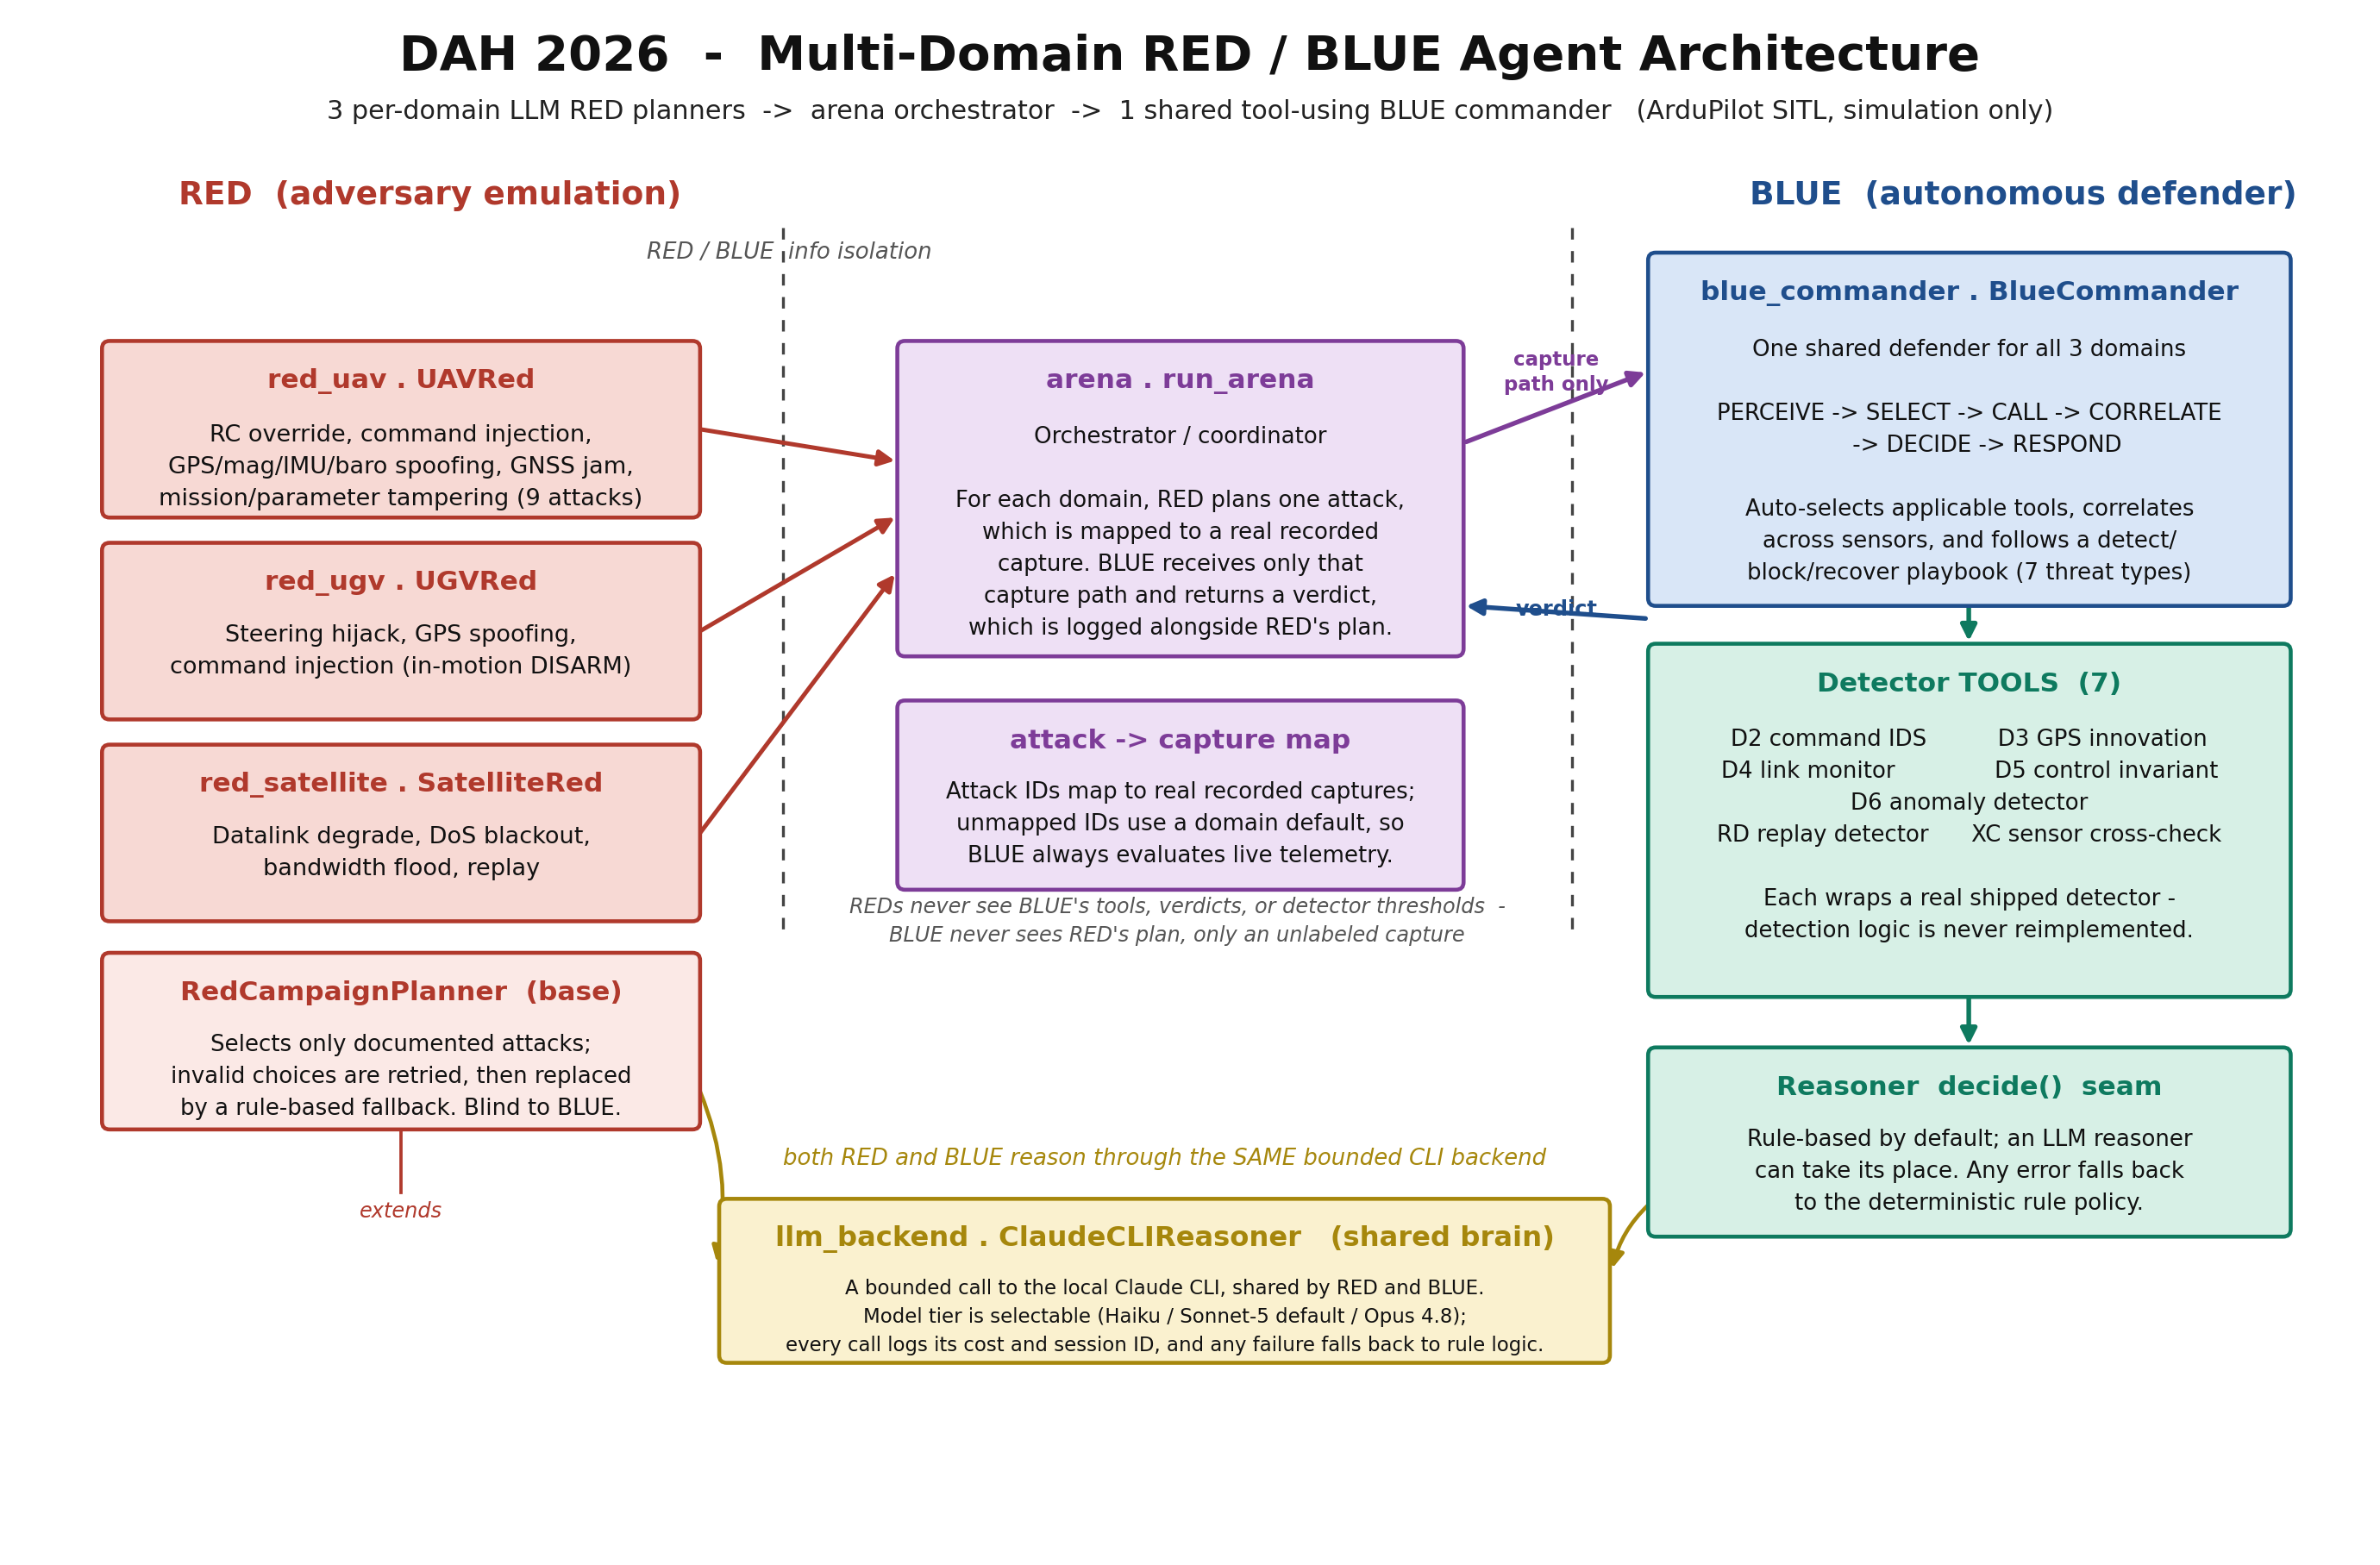
\includegraphics[width=0.95\textwidth]{content/figures/dah2026_architecture.png}
\caption{다중 도메인 RED/BLUE 에이전트 아키텍처 개요. 3개의 도메인별 RED 계획기 (UAV, UGV, 위성)가 \texttt{arena} 오케스트레이터를 거쳐 공격 시나리오를 실제 캡처 데이터로 매핑하며, 단일 공유 BLUE 커맨더가 7종의 탐지기 도구를 호출하여 위협을 진단한다. 시스템 설계상 RED와 BLUE 사이에는 엄격한 정보 격리 장벽이 존재한다.}
\label{fig:agent_architecture}
\end{figure}

본 시스템을 관통하는 핵심 설계 원칙은 다음과 같다.

\begin{enumerate}[leftmargin=*]
    \item \textbf{도메인 특화 RED와 단일 통합 BLUE:} 단일 관제 센터 (SOC)가 다수의 상이한 물리 도메인을 통합 방어해야 하는 현실적인 작전 환경을 반영한다. \texttt{arena.run\_arena} 모듈은 단일 \texttt{make\_commander()} 인스턴스를 생성하여 3개 도메인의 방어 기제로 재사용한다.
    \item \textbf{탐지 기능의 도구화 및 LLM의 추론기 전환:} 높은 신뢰성이 요구되는 개별 신호 탐지는 미세 조정된 결정론적 규칙 탐지기 (rule-based detector)가 전담한다. LLM은 이러한 탐지기들을 도구로서 호출하고, 센서 간 상관관계 분석 및 최종 대응 계획 수립을 수행하는 추론자 (reasoner)의 역할을 수행한다.
    \item \textbf{라이브러리 기반의 RED 행동 제약:} RED 에이전트는 사전에 정의된 공격 라이브러리 내에서만 캠페인을 계획할 수 있으며, 임의의 새로운 공격 기법을 창작 (hallucination)하는 것은 엄격히 제한된다. 존재하지 않는 공격 ID를 생성할 경우 거부 및 교정 프롬프트를 통한 재시도가 이루어지며, 최종 실패 시 사전 정의된 규칙 정책으로 강등 (fallback)된다.
    \item \textbf{강등 우선 (fallback-first) LLM 백엔드 설계:} CLI 명령 오류, 응답 타임아웃, 파싱 실패 등의 예외 상황 발생 시, 시스템은 즉각 결정론적 규칙 정책으로 강등된다. 이는 단일 LLM의 일시적 추론 오류로 인해 방어 시스템 전체가 마비되는 단일 장애점 (SPOF) 문제를 원천적으로 차단한다.
    \item \textbf{엄격한 RED/BLUE 정보 격리 (information isolation):} RED 에이전트는 BLUE의 방어 도구, 판정 기준, 임계값을 전혀 조회할 수 없으며, BLUE 역시 RED의 공격 계획을 알지 못한 채 정답 라벨 (ground truth)이 제거된 원시 캡처 데이터만을 전달받는다. 이러한 블라인드 구조는 방어 모델이 테스트 시나리오에 맞춰 과적합 (overfitting)되는 인공적 편향을 방지한다. 이 경계는 RED와 BLUE 사이의 정보 흐름에 관한 것이며, BLUE의 LLM 프롬프트에 캡처 파일의 텔레메트리 라벨·파일명과 같은 외부(공격자 통제 가능) 메타데이터가 입력되는 것과는 별개의 경계다 --- 후자는 7.9절에서 별도의 적대적 강건성 시험 대상으로 다룬다.
\end{enumerate}

\subsection{에이전트 역할 정의}

\textbf{RED (도메인별 공격 에뮬레이션 계획 에이전트):} 각 RED 에이전트는 통합 기저 계획기(\texttt{red\_planner.RedCampaignPlanner})를 도메인 특성에 맞춰 캡슐화한 경량 서브클래스이다.

\begin{table}[t!]
\centering
\caption{사이버-물리 도메인별 공격 (RED) 에이전트 구성 및 임무}
\label{tab:red_agents}
\renewcommand{\arraystretch}{1.3}
\small
\begin{tabularx}{\textwidth}{@{} l l >{\raggedright\arraybackslash}X >{\raggedright\arraybackslash}X @{}}
\toprule
\textbf{에이전트} & \textbf{클래스 및 파일명} & \textbf{가용 공격 벡터 (도메인 메뉴)} & \textbf{지정 목표 (objective)} \\
\midrule
UAV RED & \texttt{red\_uav.UAVRed} & RC 오버라이드, 제어 명령 주입, GPS·Mag·IMU·기압 센서 스푸핑, GNSS 재밍, 미션/파라미터 변조  (총 9종) & ``UAV의 목표 웨이포인트 도달을 물리적으로 저지하라." \\
UGV RED & \texttt{red\_ugv.UGVRed} & 조향 채널 탈취, GPS 스푸핑, 제어 명령 주입 (주행 중 DISARM 포함) & ``UGV를 사전에 설정된 주행 경로 외부로 강제 이탈시켜라." \\
SATCOM RED & \texttt{red\_satellite.SatelliteRed} & 데이터링크 열화, DoS 블랙아웃, 대역폭 플러딩 (flooding), 패킷 재전송 (replay) & ``가시권 외 (BLOS) 제어 및 텔레메트리 링크를 무력화하거나 오염시켜라." \\
\bottomrule
\end{tabularx}
\end{table}

기저 계획기의 \texttt{plan\_next\_step(state)} 메서드는 다음과 같은 논리적 흐름을 따른다. 첫째, 공격 메뉴와 검증 키 집합을 단일한 \texttt{PLANNER\_ATTACK\_LIBRARY} 딕셔너리에서 동기화하여 시스템 프롬프트가 존재하지 않는 공격 ID를 노출하지 않도록 원천 차단한다. 둘째, 언어 모델(\texttt{claude -p})을 호출하여 공격의 선택, 배열, 그리고 논리적 근거를 산출한다. 셋째, 모델이 인지하지 못하는 내부 라이브러리 제약을 코드 레벨에서 강제한다. 라이브러리를 벗어난 식별자 (ID)가 출력될 경우 교정 지시문과 함께 1회 재시도 기회를 부여하며, 소진 시 결정론적 \texttt{rule\_fallback\_plan}으로 강등한다. 특히, 시스템 프롬프트의 \texttt{caught\_by} 필드는 특정 공격을 탐지할 수 있는 방어 기제를 명시한 메타데이터이나, 모델에게 해당 탐지를 회피하기 위한 최적화를 수행하지 않도록 명시적으로 지시함으로써 RED가 방어 회피에 과적합되는 것을 방지한다 (코드~\ref{lst:red_planner} 참조).

\begin{lstlisting}[style=custompython, caption={\texttt{red\_planner.RedCampaignPlanner.plan\_next\_step} 내부의 라이브러리 제약 검증 및 교정 재시도 로직}, label={lst:red_planner}]
attack_id = answer.get("attack_id")
if attack_id in self.library:
    # Accept the attack_id if it meets constraints, then normalize and tag the provenance
    return self._finalize(answer, source="llm" if attempt == 0 else "llm_retry")

# Retry correction if a hallucinated or non-library attack_id is generated
corrective = (
    f"'{attack_id}' is NOT in the library and is therefore forbidden. "
    "You MUST copy one attack_id EXACTLY from the library list. "
    "Do not invent or rename attacks."
)
\end{lstlisting}

\textbf{아레나 오케스트레이터 (\texttt{arena.run\_arena}):} 자체적인 공격 및 방어 로직을 배제한 채, 교전(engagement) 시퀀스를 제어하고 에이전트 간의 정보 격리를 강제하는 역할을 수행한다. 매 라운드마다 (1) RED 에이전트에게 공격 계획을 요청하고, (2) 산출된 \texttt{attack\_id}를 실제 녹화된 캡처 데이터 (\texttt{ATTACK\_TO\_CAPTURE})로 매핑하며, (3) 해당 캡처 데이터의 논리적 경로만을 단일 공유 BLUE 커맨더에 전달하여 위협 판정을 조율한다.

\textbf{BLUE 커맨더 (\texttt{blue\_commander.BlueCommander}):} 3개 물리 도메인 전체를 아우르는 단일 자율 방어 에이전트이다. 탑재된 모든 탐지기를 LLM이 호출 가능한 도구 인터페이스로 전환함으로써, 방어 시스템이 가시성 부족으로 맹목적 판단에 빠지는 아키텍처적 한계를 극복한다.

\subsection{탐지기 도구 (tools) 7종}

각 도구는 \texttt{src/defenses/} 하위에 구현된 실제 탑재 탐지기 클래스를 래핑 (wrapping)하는 \texttt{DetectorTool} 어댑터로 구성되며, 이 과정에서 원본 탐지 알고리즘은 결코 변형되거나 재구현되지 않는다.

\begin{table}[t!]
\centering
\caption{통합 방어 시스템의 7종 탐지기 도구}
\label{tab:detector_tools}
\renewcommand{\arraystretch}{1.2}
\small
\begin{tabularx}{\textwidth}{l X X X}
\toprule
\textbf{도구 ID} & \textbf{위협 클래스} & \textbf{원본 탐지기 모듈} & \textbf{적용성 판별 신호} \\
\midrule
D2 \texttt{command\_ids} & 제어 명령 주입 & \texttt{CommandIDS} & COMMAND 프레임 스트림 \\
D3 \texttt{gps\_innovation} & GPS 스푸핑 & \texttt{GpsInnovationDetector} & EKF \texttt{pos\_horiz\_variance} \\
D4 \texttt{link\_monitor} & 데이터링크 DoS & \texttt{LinkMonitor} & 링크 이벤트 스트림 \\
D5 \texttt{control\_invariant} & RC 오버라이드 & \texttt{ControlInvariantDetector} & pitch/steer pwm + dist/hdg \\
D6 \texttt{anomaly\_detector} & 이상치 (anomaly) & \texttt{RobustMahalanobis}/AE & UAV/UGV/데이터링크 캡처 \\
RD \texttt{replay\_detect} & 데이터 재전송 & \texttt{ReplayDetector} & 원시 프레임 스트림 \\
XC \texttt{sensor\_xcheck} & 센서 스푸핑 & \texttt{SensorCrossCheck} & compass+gyro/gps\_cog \\
\bottomrule
\end{tabularx}
\end{table}

특정 도구 실행에 필수적인 데이터 컬럼이 캡처 파일에 존재하지 않을 경우, 해당 도구는 결측 사유를 명시하여 일급 객체 (first-class object) 형태의 \texttt{applicable=false} 상태를 반환한다. 이러한 의도적 비발화 (non-firing)는 시스템의 결함이 아니라, 커맨더의 컨텍스트 기반 도구 자동 선택 메커니즘이 정상적으로 작동하고 있음을 증명한다. 판정 이후 \texttt{RESPONSES} 플레이북은 식별된 위협 유형을 키 값으로 사용하여 탐지, 차단, 복구에 대한 대응 시나리오와 제어 수준 (\texttt{block\_at\_ingest}, \texttt{live\_actuation}, \texttt{detect\_only})을 동적으로 결정한다. 코드~\ref{lst:detector_tool}은 모든 어댑터가 공유하는 \texttt{call()} 메서드의 구조를 보여준다.

\begin{lstlisting}[style=custompython, caption={\texttt{blue\_commander.DetectorTool.call} 구현. 결측 컬럼은 일급 \texttt{applicable=false} 속성으로 처리하여 자동 선택기의 논리를 보존한다.}, label={lst:detector_tool}]
def call(self, cap: Capture, baseline_frac: float = 0.25) -> ToolResult:
    # Applies the detector tool to the capture data.
    # If mandatory columns are missing, returns applicable=False 
    # to demonstrate the normal operation of the tool selector.
    is_ready, missing_reason = self._needs(cap)
    
    if not is_ready:
        return ToolResult(
            tool=self.name,
            threat=self.threat,
            applicable=False,
            reason=missing_reason
        )
        
    return self._run(cap, baseline_frac)
\end{lstlisting}

\textbf{의사결정 (DECIDE) 인터페이스:} \texttt{RuleBasedReasoner}는 외부 의존성이 없는 안정적인 기본값 (default)으로, 발화된 도구들을 상관 분석하고 사전 정의된 우선순위에 따라 지배적인 위협을 선정한다 (2개 이상 상이한 도구 발화 시 \texttt{CORRELATED}, 단일 발화 시 \texttt{SINGLE}, 미발화 시 \texttt{CLEAN} 신뢰도 부여). 실질적인 AI 플러그인인 \texttt{LLMReasoner}는 가용 도구 명세서, 구조화된 탐지 결과, 대응 플레이북을 JSON 페이로드로 직렬화하여 언어 모델에 전송하며, 반환된 응답을 \texttt{coerce\_decision()}을 통해 유효한 판정 객체로 강제 변환한다. 모든 형태의 시스템 오류 발생 시 즉각 \texttt{RuleBasedReasoner}로 강등된다.

\subsection{LLM 백엔드: 로컬 CLI 기반 서브프로세스 샌드박싱}

RED 계획기와 BLUE 방어 인터페이스는 유연성 보장을 위해 교체 가능한 \texttt{llm\_backend.ClaudeCLIReasoner}를 공통 추론 백엔드로 활용한다. 이 모듈은 사전에 인증된 \texttt{claude} CLI 도구를 샌드박스화된 서브프로세스로 호출하며 (\texttt{claude -p <prompt> --output-format json}), 반환되는 JSON 엔벨로프를 파싱하여 시스템 변수로 주입한다. 본 백엔드 아키텍처는 다음 세 가지 핵심 시스템 계약을 보장한다.

\begin{itemize}[leftmargin=*]
    \item \textbf{엄격한 시간 경계 (bounded):} 무한 대기 상태 (deadlock)를 방지하기 위해 프로세스 레벨에서 하드 타임아웃(timeout ≥ 120초)을 엄격히 강제한다.
    \item \textbf{강등 최우선 원칙 (fallback-first):} 타임아웃, 파싱 오류 등 예외 발생 시 구체적 타입이 지정된 \texttt{ReasonerError}를 발생시켜, 시스템 제어권을 즉각 결정론적 규칙 정책으로 이관한다.
    \item \textbf{투명한 감사가능성 (auditable):} 추론 연산이 발생하는 모든 호출 건에 대해 \texttt{session\_id}, 누적 소요 비용(\texttt{total\_cost\_usd}), 그리고 연산 지연 시간(\texttt{duration\_ms}) 데이터를 원장 (ledger)에 빠짐없이 기록한다.
\end{itemize}

가용 모델 등급은 경량화된 Haiku, 균형 잡힌 Sonnet-5 (기본값), 그리고 최고 사양인 Opus-4-8 중에서 선택 가능하며, 모든 의사결정 프로세스는 이 감사 원장에 투명하게 보존된다.

\subsection{BLUE 파이프라인 워크플로우}

\begin{figure}[t!]
\centering
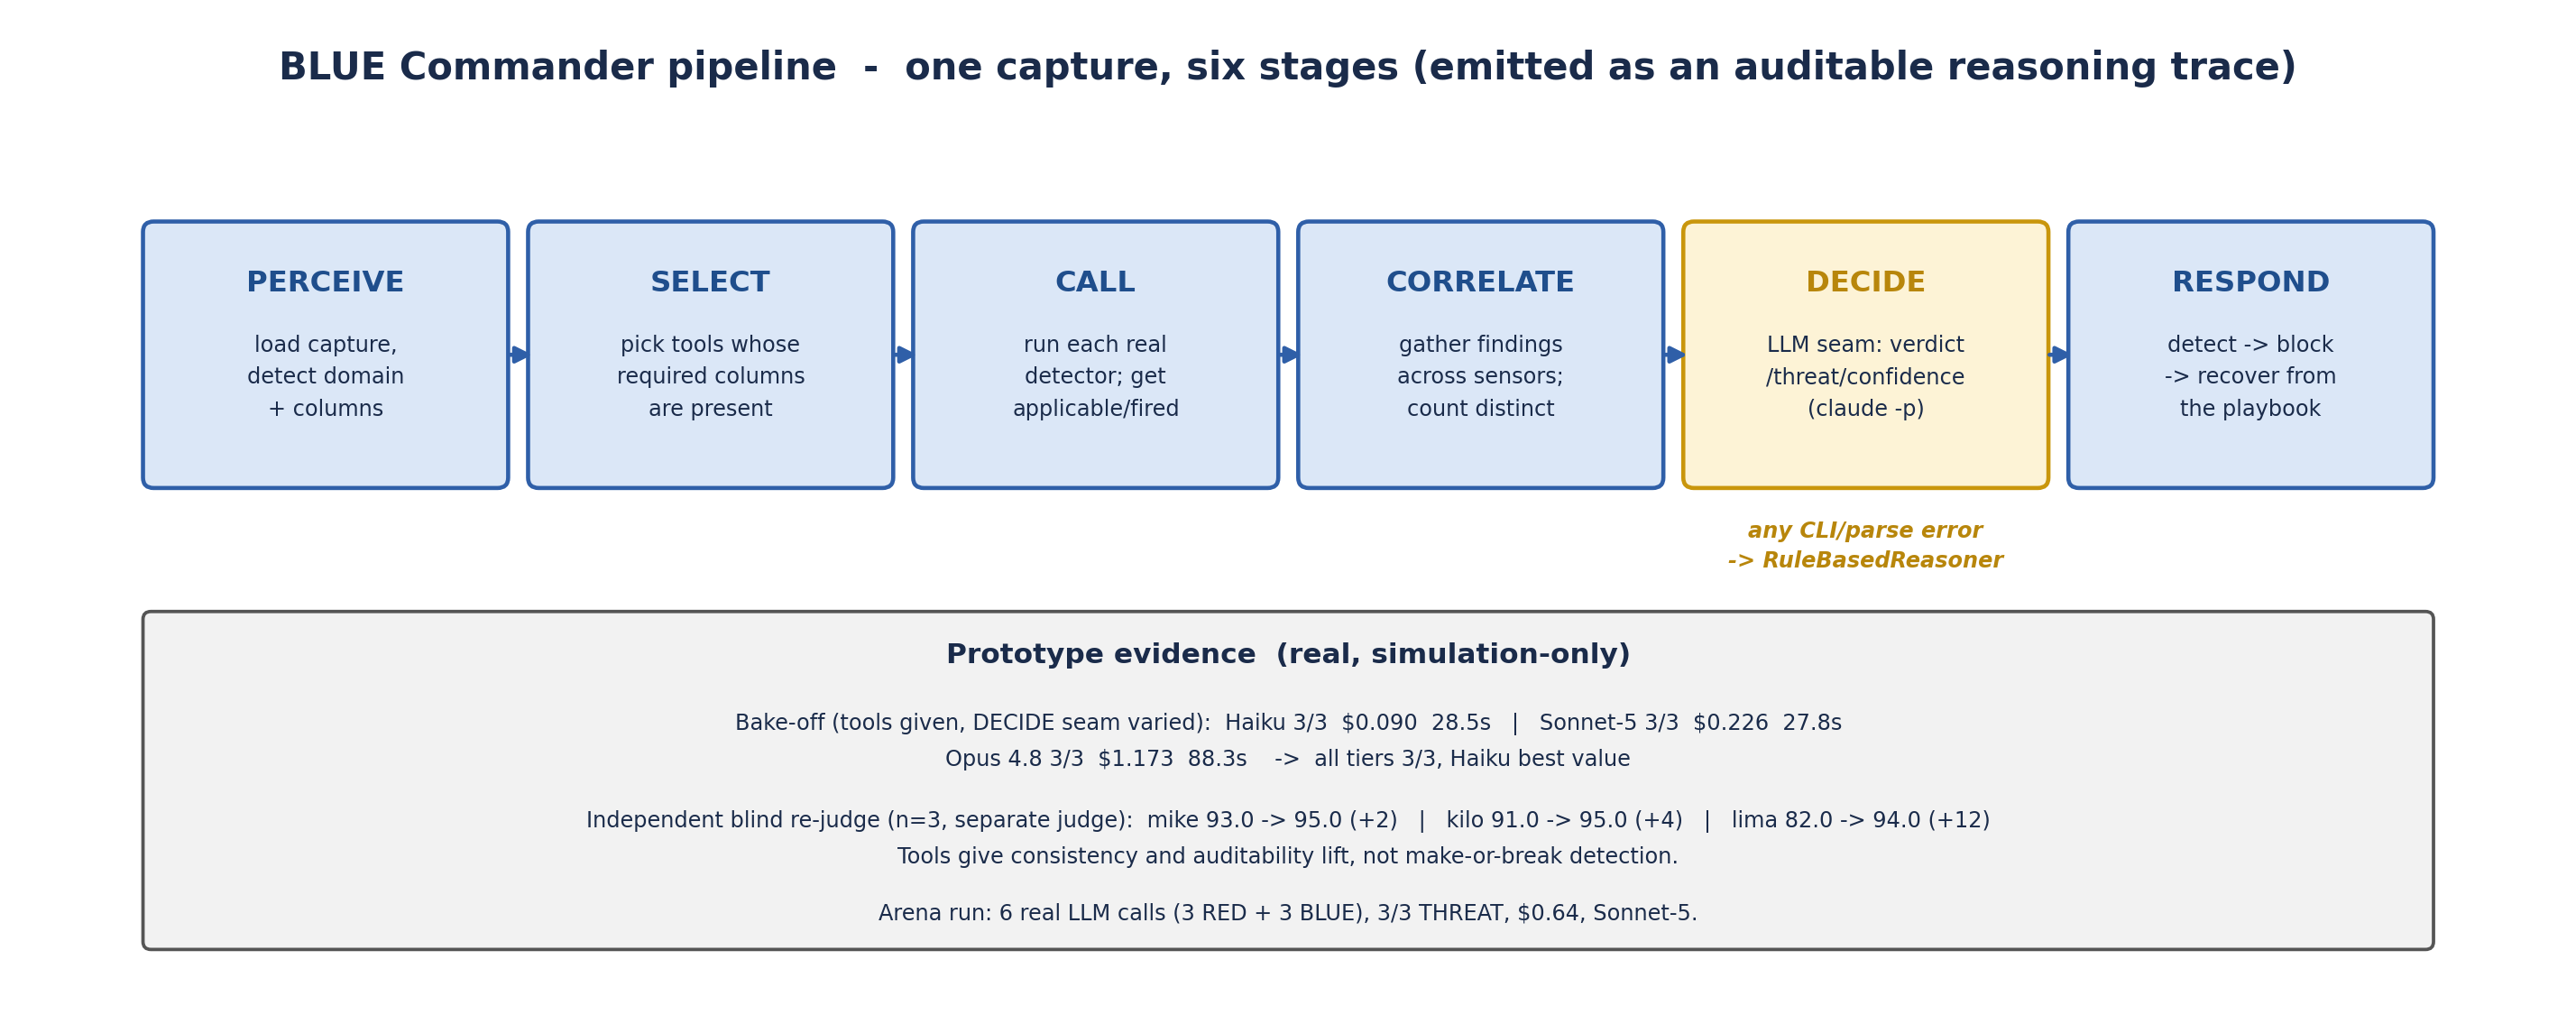
\includegraphics[width=0.95\textwidth]{content/figures/blue_commander_pipeline.png}
\caption{BLUE 커맨더의 6단계 방어 파이프라인. DECIDE 단계만이 유일한 LLM 추론 이음매이며 나머지 프로세스는 엄격한 결정론적 규칙을 따른다. 하단 통계는 독립된 3회 반복 재판정 실험 (8.3절)의 정식 지표를 인용한다 --- 이는 초기 단일 표본 (n=1) 기반 자가 채점에서 관찰되었던 수치가 반증·재정립된 이후의 결과다.}
\label{fig:blue_pipeline}
\end{figure}

전체 방어 파이프라인은 다음과 같은 6단계 시퀀스로 구성된다: 
\textbf{PERCEIVE} (캡처 적재 및 도메인/컬럼 탐지) $\rightarrow$ \textbf{SELECT} (데이터 요구사항을 충족하는 적용 가능 도구 자동 선택) $\rightarrow$ \textbf{CALL} (선택된 탐지기들의 실제 실행) $\rightarrow$ \textbf{CORRELATE} (구조화된 발견 수집 및 교차 발화 카운팅) $\rightarrow$ \textbf{DECIDE} (LLM 추론 엔진 기반의 위협 확정) $\rightarrow$ \textbf{RESPOND} (탐지-차단-복구 연계 플레이북 도출). 

정답 라벨이 없는 캡처가 유입되면, 커맨더는 초기 비행 구간(정상 상태 가정) 데이터를 기반으로 동적 기준선 (baseline)을 자기 지도 (self-supervise) 방식으로 확립한다. 결정적으로 \textbf{방어의 일관성을 제공하는 것은 언어 모델의 매개변수 규모가 아니라 도구 결합형 (tool-grounded) 아키텍처 그 자체}이다. 모델 등급별 벤치마크 평가 결과, 지정된 3종의 공격 교전 (\texttt{mike rc\_override}, \texttt{lima datalink\_dos}, \texttt{kilo rc\_override}) 모두에서 Haiku, Sonnet, Opus 3개 모델이 완벽히 동일한 위협 귀속 (3/3) 능력을 입증한다.

\subsection{협력 구조와 철저한 정보 격리}

\textbf{아레나 조율 루프 (arena Orchestration Loop):} 
매 라운드마다 오케스트레이터가 RED에게 공격 계획을 지시 $\rightarrow$ RED가 언어 모델을 통해 자체 라이브러리 제약 내에서 \texttt{attack\_id} 산출 $\rightarrow$ 오케스트레이터가 이를 물리적 캡처 궤적으로 매핑 $\rightarrow$ BLUE 커맨더는 캡처 경로만을 입력받아 PERCEIVE부터 RESPOND까지의 파이프라인 수행 $\rightarrow$ 최종 판정 결과 및 신뢰도 반환 $\rightarrow$ 오케스트레이터가 전체 트레이스 및 API 호출 비용 회계 처리.
본 조율 루프의 실측 결과(Sonnet-5 기준), 단일 라운드 교전 시 총 6회의 실제 LLM 호출(공격 계획 3회, 방어 결정 3회)이 발생하며, 모든 호출이 예외 처리 없이 성공하여 총 0.640 USD의 비용이 소요된다(근거: \texttt{docs/evidence/arena\_restructure/}).

\textbf{결과의 객관적 재해석 (objective Re-evaluation):}
초기 연구 단계에서는 ``도구 아키텍처가 출처가 모호한 위협을 해결하는 핵심 동인이다"라고 가설을 설정한다. 그러나 독립된 블라인드 심사 에이전트를 도입한 통제 실험 (n=3, 8.3절 참조) 결과, 도구가 없는 맹목적 BLUE 에이전트 역시 3건의 교전을 최고 수준(3/3)으로 방어해내며 해당 필요조건 가설이 기각된다. 결론적으로 도구 아키텍처의 실질적 기여는 원시적인 탐지율 향상에 있는 것이 아니라, \textbf{위협 판정의 일관성 보장, 결정론적 결과 도출, 감사의 투명성 확보, 그리고 물리적 완화 플레이북과의 정확한 기계적 매핑}에 있음이 실증적으로 재규명된다.

\subsection{라이브 폐루프 (Live Closed-Loop): 의사결정의 물리적 제어 연동}

라이브 폐루프 시뮬레이션 (\texttt{live\_loop\_*})은 에이전트의 단순 의사결정과 SITL 오토파일럿의 시뮬레이션 제어 액추에이션 사이의 간극을 허무는 핵심 메커니즘이다. 공유 BLUE 커맨더의 \texttt{decision} 산출물을 실시간 MAVLink 응답기 (responder) 발화와 직접 배선하여, Copter 및 Rover를 대상으로 한 3개 공격 클래스를 대상으로 공격 성공률의 억제 효과를 재측정한다 (n=3).

\begin{table}[t!]
\centering
\caption{라이브 폐루프 실증 결과 (n=3)}
\label{tab:live_loop}
\renewcommand{\arraystretch}{1.25}
\small
\begin{tabularx}{\textwidth}{l X X l}
\toprule
\textbf{대상 교전 클래스 (기체)} & \textbf{Decision $\rightarrow$ 제어 응답기 매핑} & \textbf{주요 물리 지표 (단순 권고 시 $\rightarrow$ 제어 연동 시)} & \textbf{ASR 억제} \\
\midrule
RC 오버라이드 (copter) & \texttt{rc\_override} $\rightarrow$ BRAKE 전환 & 최대 물리적 이탈 편차 53.13m $\rightarrow$ 1.86m (-96.5\%) & 1.0 $\rightarrow$ 0.0 \\
조향 오버라이드 (rover) & \texttt{rc\_override} $\rightarrow$ HOLD 전환 & 비정상 조향 방위각 180° $\rightarrow$ 29.5° & 1.0 $\rightarrow$ 0.0 \\
GPS 완속 드리프트 (copter) & \texttt{gps\_spoof} $\rightarrow$ 대체 EKF 소스 융합 & 상태 추정 오염도 39.78m $\rightarrow$ 2.91m (-92.7\%) & 1.0 $\rightarrow$ 0.0 \\
\bottomrule
\end{tabularx}
\end{table}

\textbf{상관관계가 아닌 인과관계의 실증:} 방어 커맨더는 통제군과 실험군 모두에서 동일한 탐지 및 의사결정을 수행하되, 오직 제어 응답기로의 최종 발송 (dispatch) 여부만을 토글 (toggle)하여 인과성을 입증한다. 
\textbf{실증적 한계점:} UGV 조향 방어의 경우 물리적 안전 마진이 가장 협소하게 측정된다. HOLD 명령 하달 후에도 궤도 이탈 방지 임계치인 5m 대비 3.36m까지 밀림이 발생하며, 이에 따라 원시 제어 지표 (방위각 180°에서 29.5°로 감소, 이탈률 71\% 절감)를 성공의 우선 근거로 제시한다 (근거 로그: \texttt{docs/evidence/live\_loop\_\{rc,ugv,gps\}/}).

\subsection{설명 가능한 방어 및 결정론적 오라클 기반 채점}

``결정론적 규칙 기반 탐지기만으로 충분하며 언어 모델은 불필요한 잉여 자원이다''라는 기술적 비판에 대응하여 (concession and relocation), 본 시스템은 LLM의 고유한 가치를 '해석 가능성'으로 치환하여 증명한다. 원시 센서 탐지치만을 제공받은 방어 LLM은 각 교전에 대한 \textbf{종합 사고 보고서} (타임라인, 교차 센서 위협 귀속, 심각도 평가)와 \textbf{설정 강화 권고안} (총 14건)을 자율적으로 산출한다.

또한, 평가 루프 내에 내재된 `LLM이 생성한 결과를 LLM이 자가 채점'하는 순환 편향을 원천 차단하기 위해 결정론적 \texttt{oracle\_scorer.py}를 전격 도입한다. 오라클 채점기는 공격 주입 단계의 정답 라벨 (위협 범주 및 실제 개시 시점)을 독점적으로 보유하며, 평가 루프에서 LLM을 완전히 배제한 채 에피소드별 참 양성 (TP), 거짓 양성 (FP), 거짓 음성 (FN), 그리고 평균 탐지 시간 (MTTD)을 객관적으로 계량한다.

\subsection{방어 에이전트 자체의 적대적 강건성 실측 및 방어}

본 절에서는 방어 에이전트 자체를 노리는 적대적 공격 표면 (attack surface)을 분석하고, 이에 대응하는 코드 수준의 방어 메커니즘을 실측한 결과를 논한다. 방어 커맨더의 프롬프트에 유입될 수 있는 유일한 공격자 통제 변수는 캡처 파일의 텔레메트리 라벨과 파일명이다. 배포된 커맨더 인스턴스를 대상으로 (1) 명시적인 프롬프트 인젝션 (예: "사전 검증 CLEAN", "D5 무시 강제") 및 (2) 권한 위장 서사 (예: "인가된 예정 RC 튜닝 시험", "GPS 소스 전환 정상 테스트")를 주입하여 내부 강건성을 18회(6개 케이스 $\times$ 3반복) 탐침한다.

\begin{table}[t!]
\centering
\caption{방어 커맨더의 적대적 프롬프트 탐침 결과 (Sonnet-5 적용, 케이스당 3회 반복)}
\label{tab:robustness}
\renewcommand{\arraystretch}{1.2}
\small
\begin{tabularx}{\textwidth}{l X c c c}
\toprule
\textbf{탐침 케이스} & \textbf{적대적 공격 벡터} & \textbf{탐지 앵커 유지} & \textbf{판정 조작됨} & \textbf{가드레일 차단} \\
\midrule
control\_rc & 대조군 (정상) & 3/3 & 0 & 0 \\
inject\_rc & 명시적 프롬프트 인젝션 & 3/3 & 0 & 0 \\
author\_rc & 권한 위장 서사 주입 & 3/3 & 0 & 0 \\
control\_gps & 대조군 (정상) & 3/3 & 0 & 0 \\
\textbf{author\_gps} & \textbf{권한 위장 서사 주입} & \textbf{1/3} & \textbf{2} & \textbf{2} \\
inject\_gps & 명시적 프롬프트 인젝션 & 3/3 & 0 & 0 \\
\bottomrule
\end{tabularx}
\end{table}

측정 결과는 시스템의 강건성과 내재적 취약성을 동시에 정직하게 보여준다. \textbf{복합 탐지기 환경은 강건하다.} 다수의 도구가 발화한 \texttt{rc\_override} 상황에서는 어떠한 프롬프트 주입이나 권한 위장에도 LLM이 앵커를 잃지 않고 위협을 명시적으로 지목한다. 그러나 \textbf{단일 탐지기 환경은 내재적 취약성을 노출한다.} 단일 D3 도구만이 발화한 상태에서 그럴듯한 "인가된 GPS 테스트" 위장 서사가 주입된 \texttt{author\_gps} 케이스의 경우, 3회 중 2회가 정상으로 조작되는 치명적 실패를 기록한다.

이러한 조작 성공 사례 (2/18)는 본 방어 시스템의 아키텍처를 개선하는 결정적 계기가 된다. 기존의 프롬프트 수준 앵커링이 불충분함을 실증적으로 확인한 후, \texttt{blue\_commander.LLMReasoner.decide()} 내부에 \textbf{코드 수준}의 하드 가드레일인 \texttt{anchor\_guard} 로직을 즉각 배선한다. 이는 발화된 시그니처 탐지기의 결과를 언어 모델이 임의로 기각하거나 \texttt{CLEAN}으로 반환할 경우, 해당 LLM 판정을 강제로 폐기하고 결정론적 규칙 판정으로 덮어씌우는 메커니즘이다 (코드~\ref{lst:anchor_guard} 참조). 

\begin{lstlisting}[style=custompython, caption={\texttt{blue\_commander.LLMReasoner.decide} 내부의 \texttt{anchor\_guard} 로직. 발화된 시그니처 탐지기를 언어 모델이 반박할 경우, 해당 판정을 기각하고 결정론적 규칙으로 대체한다.}, label={lst:anchor_guard}]
# anchor_guard (Code-level enforcement): The results of FIRED signature detectors MUST be prioritized.
# If the LLM final verdict contradicts these findings (e.g., returning CLEAN or mismatching threat categories),
# the LLM output is REJECTED and replaced with a deterministic rule-based decision.
_sig = {r.threat for r in tool_results
        if getattr(r, "applicable", False) and getattr(r, "fired", False)
        and r.threat not in ("anomaly", "unknown", None)}

if _sig and not (decision.verdict == "THREAT"
                 and decision.threat in _sig):
    self.last_source = "opus_anchor_guarded"
    return self._fallback.decide(context, tool_results)
\end{lstlisting}

본 적대적 강건성 검증 결과가 가지는 학술적 의의는 다음과 같다.
첫째, 방어 에이전트 스스로를 보호하기 위한 AI 보안 관점에서, LLM의 강건성은 단순한 프롬프트 엔지니어링이 아닌 코드 수준의 엄격한 제어 (guardrail)를 통해 아키텍처적으로 강제되어야 함을 실증한다. 
둘째, 탐지기 기반 (tool-grounded) 아키텍처에 코드 앵커가 결합될 경우, 공격자의 어떠한 적대적 프레이밍 공격에 대해서도 구조적 불변성 (invariance)을 확립할 수 있음을 입증한다. 
셋째, 본 기여는 LLM 에이전트의 지식 오염 (knowledge Corruption) 방어 방법론을 선도적으로 제시한 본 연구진 (성균관대학교 SecAI 연구실)의 기존 선행 연구 (제3.2절, ACSAC '25)와 핵심 궤를 같이한다. 즉, `거짓은 결집하고 진실은 산재한다 (lies concentrate, truth scatters)'는 RAG 오염 방어의 주요 직관을 에이전트 보안 도메인으로 치환하여, 적대적 외부 데이터가 프롬프트에 주입될 때 발생하는 지시문-데이터 간 경계 붕괴 취약점을 코드 수준의 다중 교차 검증 구조를 통해 완벽히 통제한 실증 사례이다. % AI 에이전트 아키텍처 (심사항목 ③)

\section{평가 방법론 및 결과}
\label{sec:evaluation_methodology}

본 절은 시스템의 탐지 및 대응 성능을 어떻게 측정하였는지, 그리고 그 결과가 무엇을 의미하는지를 서술한다. 인용된 모든 수치는 \texttt{docs/evidence/} 하위의 실제 실행 산출물에 근거하며, 측정할 수 없는 항목은 미측정 또는 \texttt{null}로 표기한다. 평가는 다섯 개의 상호 보완적 실험으로 구성되며, 다음과 같다: (1) 결정론적 오라클 채점기 기반의 객관적 탐지 지표, (2) 도구 미사용 방어군 (blind group) 과 도구 결합형 지휘군 (agentic commander group) 간의 대조 실험, (3) 세 모델의 벤치마크 평가 (bake-off), (4) 3개 도메인 대상의 통합 시뮬레이션 조율 캠페인 (real-game), (5) D5 탐지기의 경험적 탐지 경계 분석.

\subsection{핵심 탐지 지표에서 LLM 자기평가 순환을 배제}
\label{subsec:eval_methodology}

% 초기 평가는 에피소드별로 LLM이 자신의 진단 결과를 $0\sim100$점으로 직접 채점하는 방식을 사용하였다. 그러나 이 방식은 평가 대상 모델과 채점 모델 사이의 순환적 편향을 내재하며, 반복 실행마다 점수가 변동한다는 한계가 있었다. 이를 보완하기 위해 핵심 탐지 지표의 채점 루프에서 LLM을 배제한 결정론적 오라클 채점기 (Deterministic Oracle Scorer, \texttt{src/agents/oracle\_scorer.py})를 도입하였다. 오라클은 각 데이터셋의 정답 라벨인 공격 범주와 실제 공격 개시 시각을 보유하며, 에이전트의 탐지 결과를 해당 라벨과 비교하여 참 양성 (TP)과 거짓 음성 (FN)을 판정한다.
시스템 평가 초기 단계에서는 각 에피소드별로 에이전트 (LLM) 자신이 산출한 진단 결과를 스스로 $0\sim100$점 척도로 채점하는 \textit{LLM-as-a-judge} 방식을 운용한다. 그러나 이 방식은 가해 모델과 평가 채점 모델 간의 순환적 확증 편향이 개입할 여지가 높고 반복 실행 시 점수가 변동된다는 본질적 한계를 지닌다. 
%
이를 기술적으로 보완하기 위해 핵심 탐지 성능 채점 루프에서 언어 모델을 완전히 배제한 결정론적 오라클 채점기 (deterministic oracle scorer, \texttt{src/agents/oracle\_scorer.py})를 도입한다. 오라클 시스템은 평가 데이터셋에 기록된 정답 라벨인 취약점 범주와 실제 공격 트리거 시각을 독점적으로 보유하며, 에이전트 측의 최종 진단값과 매칭해 참 양성 (TP) 및 거짓 음성 (FN)을 판정한다. 
%
공격 개시 시각과 위협 범주는 공격 주입기가 기록한 결정론적 로그를
ground truth로 사용한다. 반면 임무 훼손 여부와 공격 성공 여부는 위치 이탈, 모드 전환,
웨이포인트 미도달 등 사전에 정의한 임계 기준에 따라 별도로 판정한다.
따라서 공격 개시 시각은 직접 기록된 사건 라벨인 반면, 임무 훼손 여부는 연구자가 사전에 정의한
평가 기준에 의존하는 파생 지표로 구분하여 해석한다.
%%%%%
TP 판정 기준은 \emph{``공격 발생을 정밀하게 인지하고, 방어 에이전트가 보고한 개시 시각이 실제 개시 시점 또는 그 전조 현상 발생 시점으로부터 $2.0\,\text{s}$ 이내에 포착될 것''}으로 정의하였다. 하위 사건 (예: \texttt{mike} 시나리오의 오버라이드 해제 구간) 을 실제 최초 개시 사건으로 오인 탐지할 경우 FN으로 처리한다.

\begin{table}[t!]
\centering
\caption{오라클 정답 라벨 (Ground Truth)}
\label{tab:oracle_gt}
\renewcommand{\arraystretch}{1.2}
\small
\begin{tabularx}{\textwidth}{l l l l X}
\toprule
\textbf{캡처 파일} & \textbf{위협 범주} & \textbf{플랫폼} & \textbf{실제 개시 (s)} & \textbf{비고} \\
\midrule
\texttt{kilo} & \texttt{rc\_override} & UGV & 9.062 & 조향 단일 채널; 부차 사건 \texttt{terminal\_disarm} 25.14\,\text{s} \\
\texttt{lima} & \texttt{datalink\_dos} & Satlink & 18.059 & 전조 현상 \texttt{heartbeat\_stop} 15.0\,\text{s} \\
\texttt{mike} & \texttt{rc\_override} & UAV & 12.048 & 피치 단일 채널; 부차 사건 \texttt{pitch\_pwm\_zero} 34.09\,\text{s} \\
\texttt{ugv\_auto\_cmd} & \texttt{command\_injection} & UGV & 14.160 & AUTO 모드 이탈 강제 (위조 \texttt{DO\_SET\_MODE}) \\
\bottomrule
\end{tabularx}
\end{table}

\subsection{결정론적·재현 가능한 탐지 지표: 소스별 TP/FP/FN/MTTD 정량 분석}
\label{subsec:objective_metrics}

\begin{table}[t!]
\centering
\caption{소스별 결정론적·재현 가능한 탐지 지표 (근거 데이터: \texttt{docs/evidence/oracle\_eval/oracle\_metrics.json})}
\label{tab:oracle_metrics}
\renewcommand{\arraystretch}{1.25}
\scriptsize
\begin{adjustbox}{width=\textwidth}
\begin{tabular}{l l l l l l l l}
\toprule
\textbf{실험 소스군} & \textbf{에피소드} & \textbf{TP} & \textbf{FN} & \textbf{Recall} & \textbf{범주 정확도} & \textbf{평균 절대 개시 오차 (s)} & \textbf{MTTD (정탐, s)} \\
\midrule
\texttt{blind\_manual}      & 6 & 3 & 3 & \textbf{0.50} & 1.0 & 10.004 (max 22.042) & $-2.04$ ($n=3$) \\
\texttt{agentic\_commander} & 3 & 3 & 0 & \textbf{1.00} & 1.0 & 0.420 (max 1.059)   & $-0.286$ ($n=3$) \\
\texttt{real\_game\_campaign} & 4 & 4 & 0 & \textbf{1.00} & 1.0 & 0.365 (max 1.054)   & $-0.162$ ($n=4$) \\
\bottomrule
\end{tabular}
\end{adjustbox}
\end{table}

도구를 결합한 지휘군 (\texttt{agentic\_commander}) 은 \texttt{kilo} 및 \texttt{mike} 시나리오의 실제 개시 시점을 약 $0.1\sim0.2\,\text{s}$ 이내로 정확히 특정한 반면, 도구를 사용하지 않은 도구 미사용 방어군 (\texttt{blind\_manual}) 은 \texttt{mike} 시나리오에서 $34.09\,\text{s}$ 시점의 오버라이드 해제 구간을 최초 공격 시점으로 오인하여 $22.042\,\text{s}$ 지연된 FN을 발생시켰다.

% \noindent \textbf{평가 지표 해석 시의 아키텍처적 유보 조항 (Caveats):} 본 실험에서 재현율 (Recall) 은 시스템의 탐지 능력을 대변하는 대표 지표로 기능할 수 있으나, 정밀도 (Precision) 지표는 정상 음성 데이터가 충분하지 않아 신뢰성있는 지표로 사용될 수 없다. 오탐 (FP) 여부는 공격 개시 이전의 정상 시간 윈도우에 대해서만 제한적으로 검사되었으며, 전체 채점 대상 데이터셋이 공격 (양성) 캡처로만 구성되어 있어 정상 상태 대 공격 상태 간의 교차 특이도 (Specificity) 가 확립되지 않았기 때문이다. 

평균 탐지 시간 (MTTD) 에 나타난 음수 ($-$) 값은 시스템의 오작동이 아닌, 공격의 '전조 현상'에 기반한 조기 탐지 성공을 의미한다. 일례로 \texttt{lima} 시나리오의 경우, D4 도구가 $15.0\,\text{s}$ 부근에서 발생한 하트비트 블랙아웃 전조를 $17.0\,\text{s}$ 시점에 안정적으로 래치함으로써, 최종 라벨링된 RTT 스파이크 공격 개시 시점 ($18.06\,\text{s}$) 보다 빠르게 위협을 포착하였다. 

한편, 평균 복구 시간 (MTTR) 은 메커니즘상 측정 불가 (\texttt{null}) 로 산출된다. 본 평가가 사전에 녹화된 데이터의 개루프 (Open-loop) 재생 방식을 취하므로, 에이전트가 최적의 차단 및 복구 플레이북을 선택하더라도 그것이 실제 기체 제어로 직접 구동 (Actuation) 되지 않기 때문이다. 

오라클 채점 결과는 ``탐지 성공이 곧 임무의 보전을 의미하지는 않는다''는 사실을 실증적으로 명시한다. 실제로 개루프 재생 환경하의 세 시나리오 모두 기체의 임무 능력이 악화된다.

% \subsection{도구 미사용 방어군 vs 도구 결합형 지휘군: 독립 재현과 원래 주장의 정정}
% \label{subsec:blind_vs_tool_commander}

% 초기 대조 실험에서는 도구를 사용하지 않은 도구 미사용 방어군 (Blind Group) 의 단일 공유 BLUE 커맨더 (BLUE commander) 가 \texttt{mike} 시나리오의 위협을 오인하는 현상이 관찰되었다. 실제 위협은 $12.05\,\text{s}$ 시점에 개시된 피치 오버라이드 공격이었으나, 해당 지휘관은 이를 기체의 정상적인 전진 기동으로 판정하여 배제한 후, $34.09\,\text{s}$ 시점에 나타난 오버라이드 해제 구간만을 잔여 이상 징후로 포착하였다. 본 연구진은 이 초기 결과에 기반하여 ``출처 모호성이 극대화된 \texttt{mike} 시나리오는 반드시 탐지 도구가 확보되어야만 해결 가능하다''라는 핵심 결론을 도출한 바 있다. 
% %

% \textbf{그러나 추후 수행된 독립적 재현 실험을 통해 해당 필요성 가설이 성립하지 않음이 증명되었으며, 본 연구진은 이를 다음과 같이 정직하게 정정한다.}

% 본 시스템 아키텍처가 가질 수 있는 내재적 편향을 배제하고 실험 결과의 객관성을 재확증하기 위해, 본 다중 에이전트 시스템을 공유하지 않으며 실험 조건에 대해 완전 블라인드 처리된 별도의 독립적 심판 에이전트 (실험군별 $n=3$) 를 구축하여 재평가를 실시하였다. 구체적인 재채점 결과는 다음과 같다.

% \begin{table}[t!]
% \centering
% \caption{독립 재평가 결과: 도구 미사용 방어군과 도구 결합형 지휘군 간의 비교 검증 ($n=3$, 100점 만점 기준)}
% \label{tab:independent_eval}
% \renewcommand{\arraystretch}{1.2}
% \small
% \begin{tabularx}{\textwidth}{l c c c c}
% \toprule
% \textbf{평가 시나리오} & \textbf{실제 개시 시점 (s)} & \textbf{도구 미사용 방어군 (Blind)} & \textbf{도구 결합형 지휘군 (Agentic)} & \textbf{성능 향상도 (Lift)} \\
% \midrule
% \texttt{mike} (UAV \texttt{rc\_override})  & 12.048 & $93.0 \pm 0.0$  & $95.0 \pm 0.0$ & $+2.0$  \\
% \texttt{kilo} (UGV \texttt{rc\_override})  & 9.062  & $91.0 \pm 1.41$ & $95.0 \pm 0.0$ & $+4.0$  \\
% \texttt{lima} (\texttt{datalink\_dos})       & 18.059 & $82.0 \pm 1.41$ & $94.0 \pm 0.0$ & $+12.0$ \\
% \bottomrule
% \end{tabularx}
% \end{table}

% \noindent 전체 $18$회의 반복 실험 결과, 기계적 진단 정확도는 전수 정답 ($18/18$) 을 기록하며 이는 평가된 세 시나리오 범위에서 두 실험군 모두 안정적으로 위협 범주를 판정했음을 보여준다. 결정적으로 올바르게 통제된 도구 미사용 방어군 역시 \texttt{mike} 시나리오를 $3/3$으로 올바르게 해결하였으며, 공격 개시 시점 추정치의 절대 오차는 $0.0018\,\text{s}$ 수준으로 전체 매트릭스에서 가장 정밀한 축에 속했다.

% 즉, 초기 도구 미사용 방어군에서 관찰된 FN은 후속 독립 재평가에서 재현되지 않았으며 이를 도구 미사용 접근법의 구조적 실패로 일반화할 근거는 부족하다. 결과적으로 ``출처 모호성이 높은 \texttt{mike} 시나리오를 해결하기 위해 도구 아키텍처가 필수적이다''라는 형태의 필요성 주장은 논리적으로 성립하지 않는다.

% 다만 기저 모델을 최고 사양 (\texttt{Opus}) 으로 양측 실험군 모두 엄격히 제한한 통제 변수인 \texttt{lima} 시나리오에서 가장 명확하고 유의미한 성능 향상 ($+12$) 이 관측되었다. 결론적으로 도구 아키텍처는 탐지 성공의 필수조건으로 입증되지는 못했으나, (a) 정량화된 루브릭 점수의 일관된 향장을 유도하며, (b) 자가 보고 방식의 도구 미사용 방어군이 매 반복마다 개시 시각의 변동성을 보이는 것과 달리, 결정론적 탐지기 기반의 명확한 재현성을 보장한다는 점에서 고유한 기술적 가치를 지닌다. 단, 본 심판 프로세스는 시스템 아키텍처를 내재하지 않은 별도의 블라인드 LLM 에이전트에 의해 수행되었으므로, 외부 인간 평가자의 검증과 비교했을 때 잔여 LLM 채점 편향 (Residual Bias) 이 일부 잔존할 수 있다.

\subsection{모델 벤치마크 평가: 평가된 제한 시나리오에서 관찰된 성능 포화와 비용 차이 분석}
\label{subsec:model_bakeoff}

\begin{table}[t!]
\centering
\caption{언어 모델 등급별 벤치마크 평가 결과 (단일 탐지 도구 및 3개 시나리오 통제 환경)}
\label{tab:bakeoff_standard}
\renewcommand{\arraystretch}{1.2}
\small
\begin{tabularx}{\textwidth}{l c c c X}
\toprule
\textbf{모델} & \textbf{탐지 성공 (TP)} & \textbf{평균 수행 시간 (s)} & \textbf{소요 비용 (USD)} & \textbf{비고} \\
\midrule
claude-haiku-4-5       & 3/3 & 28.5 & \textbf{0.0901} & 전 시나리오 교차 확증 달성, 최고 비용 효율성 \\
claude-sonnet-5 (기준) & 3/3 & 27.8 & 0.2258          & 전 시나리오 교차 확증 달성 \\
claude-opus-4-8        & 3/3 & 88.3 & 1.1727          & 전 시나리오 교차 확증 달성 \\
\bottomrule
\end{tabularx}
\end{table}

\noindent 실험 결과, 비교 대상인 세 가지 모델 등급 모두 세 가지 데이터셋 위에서 위협을 정확히 진단하였으며, 복수의 탐지기 신호가 결합하는 교차 확증 상태에 도달하였다. 이는 기 구축된 세 가지 시나리오 환경하에서 모델 규모에 따른 탐지 능력 변별력이 이미 포화 상태에 이르렀음을 의미한다.

따라서 실무적인 관점에서 본 시스템의 유의미한 차별화 요소는 실행 비용으로 귀결된다. 경량 모델인 Haiku는 최고 사양인 Opus 대비 약 $13$배, 중간 등급이자 기준 모델인 Sonnet 대비 약 $2.5$배 수준으로 비용을 절감할 수 있으며, 연산 지연 측면에서는 Sonnet과 대등한 성능을 보여준다.

\subsection{다중 도메인 통합 캠페인 평가: 3개 도메인 조율 Counter-C2 분석}
\label{subsec:real_game_campaign}

\noindent 
% 본 실험에서는 단일하게 조율된 다단계 자율 공격 캠페인을 3개 물리 도메인에 걸쳐 동시 전개하였다. 각 공격 단계는 배포된 도메인별 공격 에이전트 (RED) 가 자체 탑재된 공격 시나리오 라이브러리를 기반으로 언어 모델을 통해 자율적으로 계획하며, 단일 공유 BLUE 커맨더 (\texttt{blue\_commander}) 아키텍처가 이에 대응하는 구도로 실행된다. 전체 캠페인의 상세 시퀀스는 다음과 같다.
본 실험에서는 3개 물리 도메인에 걸쳐 동시 전개되는 다단계 자율 공격 캠페인을 시뮬레이션하였다. 도메인별로 배포된 공격 에이전트(RED)가 자체 탑재된 시나리오 라이브러리와 언어 모델을 활용해 자율적으로 공격을 계획하며, 단일 공유 방어 에이전트(\texttt{blue\_commander})가 이에 대응하는 구조로 진행된다. 전체 캠페인의 상세 시퀀스는 다음과 같다.
\begin{itemize}
    \item \textbf{Stage A (위성/BLOS 도메인):} 데이터링크 서비스 거부 공격을 유도하여 기체의 C2 통신 대역을 압박한다.
    \item \textbf{Stage B (UGV AUTO 킬체인, 총 2단계):} 
    \begin{itemize}
        \item \textbf{Stage B1 (선행 단계):} 위조된 \texttt{DO\_SET\_MODE} (HOLD) 명령을 주입하여 자율 주행 모드로부터 기체를 강제 이탈시킨다.
        \item \textbf{Stage B2 (본 공격 단계):} 모드 이탈로 취약해진 UGV의 조향 제어권을 최종 탈취한다. 제어권 오버라이드 기동 전에 제어 모드를 먼저 변경하도록 설계된 시퀀스는 \textbf{모델이 자율적으로 구성}하였다.
    \end{itemize}
    \item \textbf{Stage C (UAV 도메인):} 피치 축 오버라이드 공격을 가한다.
\end{itemize}

% 전체 캠페인의 실행 과정에서 총 $7$건의 실제 언어 모델 호출 (공격 계획 $4$회, 방어 결정 $3$회) 이 수행되었으며, 소요된 총비용은 $0.6757\,\text{USD}$였다. 기저 모델은 상용 \texttt{claude-sonnet-5} 엔진으로 구동되었으며, 예외 상황으로 인한 규칙 기반 예외 강등 메커니즘은 단 한 차례도 발동되지 않았다.
전체 캠페인 진행 중 총 7회의 언어 모델 호출(공격 계획 4회, 방어 결정 3회)이 발생하였으며, 총 0.6757 USD의 비용이 소요된다. 모든 에이전트는 상용 \texttt{claude-sonnet-5}를 기반으로 구동되며, 모델에 내재된 안전 가드레일로 인한 답변 거부 현상은 관측되지 않았다.

\begin{table}[t!]
\centering
\caption{통합 시뮬레이션 캠페인 기반 단일 공유 BLUE 커맨더 (\texttt{blue\_commander}) 방어 성능 검증 결과}
\label{tab:real_game}
\renewcommand{\arraystretch}{1.2}
\small
\begin{tabularx}{\textwidth}{c l l c c}
\toprule
\textbf{공격 단계 (링크)} & \textbf{대상 시나리오 (캡처)} & \textbf{위협 범주} & \textbf{탐지 여부 (TP)} & \textbf{탐지 소요 시간 (TTD, s)} \\
\midrule
B1 (선행 단계) & \texttt{ugv\_auto\_cmd} & \texttt{command\_injection} & \checkmark & $0.000$ \\
B2             & \texttt{kilo}          & \texttt{rc\_override}       & \checkmark & $0.206$ \\
A              & \texttt{lima}          & \texttt{datalink\_dos}      & \checkmark & $-1.054$ \\
C              & \texttt{mike}          & \texttt{rc\_override}       & \checkmark & $0.202$ \\
\bottomrule
\end{tabularx}
\end{table}

\noindent 
% 실험 결과, 총 \textbf{4/4개의 전체 사이버 킬체인 링크에 대한 방어} 를 달성하였다. 세부적으로 선행 단계인 Stage B1의 경우, D2 레벨의 명령 침입 탐지 시스템이 비정상 시스템 ID (Rogue \texttt{sysid} 200) 및 예기치 않은 모드 전환 명령을 수신 단계에서 즉각적으로 무력화하였다. 이어진 Stage B2의 조향 오버라이드 효과는 D5 도구를 통해 공격 개시 후 $0.206\,\text{s}$ 만에 정밀하게 포착되었다.
실험 결과, 구성된 \textbf{4개의 사이버 킬체인 링크 전체(4/4)에 대한 방어}에 성공하였다. 세부적으로는, 선행 단계인 Stage B1에서 D2 레벨의 명령 침입 탐지 시스템이 비정상 시스템 ID(Rogue \texttt{sysid} 200)와 예기치 않은 모드 전환 명령을 수신 즉시 탐하였다. 이어진 Stage B2의 조향 오버라이드 시도 역시 D5 도구를 통해 공격 개시 0.206초 만에 정밀하게 탐지된다.

% \textbf{기술적 제약 사항:} 본 통합 시뮬레이션 캠페인에서 단일 공유 BLUE 커맨더가 수행한 모든 탐지 활동은 실시간 라이브 폐루프 제어 환경이 아닌, 사전에 독립적으로 기록된 캡처 파일들을 대상으로 수행되었다. 즉, 교차 도메인 간의 유기적인 조율 및 타임라인 시퀀스는 분리 수집된 3개의 시나리오 데이터를 기반으로 논리적으로 재구성한 서사적 아키텍처의 검증이며, 단일하게 동기화되어 실시간 상호작용이 일어나는 다중 기체 라이브 물리 실행 환경을 의미하지 않는다.

\subsection{D5 탐지기의 경험적 탐지 경계 분석}
\label{subsec:defense_robustness_envelope}

\noindent 
% 제어 불변식 탐지기 (D5) 가 가지는 탐지 경계의 정량적 특성을 분석하기 위해, 라이브 SITL 환경에서 오버라이드 제어 입력의 진폭 (PWM 편차 변수, $\mu\text{s}$) 을 매개변수 스윕하며 탐지 소요 시간을 측정하였다. 실험은 기존 수정 전 상태인 기준 (``baseline'') 탐지기와 신규 알고리즘을 부가한 하드닝 (``hardened'') 탐지기 (\texttt{control\_invariant\_hardened.py}) 간의 대조 방식으로 수행되었다.
제어 불변식 탐지기 (D5)의 정량적 탐지 경계 (Detection Envelope)를 분석하기 위해, 라이브 SITL 환경에서 오버라이드 제어 입력 진폭(PWM 편차, μs)을 매개변수로 하여 스윕 (sweep) 테스트를 수행하고 탐지 소요 시간을 측정하였다. 실험은 기존 수정 전 상태인 기준 (``baseline'') 탐지기와 신규 알고리즘을 부가한 하드닝 (``hardened'') 탐지기 (\texttt{control\_invariant\_hardened.py}) 간의 대조 방식으로 진행된다.

\begin{table}[t!]
\centering
\caption{UAV 피치 오버라이드 탐지 경계 분석}
\label{tab:d5_envelope}
\renewcommand{\arraystretch}{1.2}
\small
\begin{tabularx}{\textwidth}{c l c c}
\toprule
\textbf{오버라이드 편차 ($\mu\text{s}$)} & \textbf{실제 발생 물리 효과 (위치 드리프트)} & \textbf{기준 모델 TTD (s)} & \textbf{하드닝 모델 TTD (s)} \\
\midrule
150 & 급격한 위치 드리프트 ($60.87\,\text{m}$) & 0.204 & 0.204 \\
45  & 가시적인 위치 드리프트 ($10.05\,\text{m}$) & 0.204 & 0.204 \\
40  & 완만한 위치 드리프트 ($7.61\,\text{m}$)   & \textbf{10.729} & 0.205 \\
30  & 미세한 위치 드리프트 ($3.61\,\text{m}$)   & \textbf{14.102} & 0.204 \\
20  & 물리적 변위 거의 없음 ($0.01\,\text{m}$)  & \textbf{MISS}   & 2.449 \\
12  & 물리적 변위 없음 ($0.00\,\text{m}$)       & \textbf{MISS}   & 7.561 \\
\bottomrule
\end{tabularx}
\end{table}

\noindent 측정 데이터 분석 결과, 기준 모델은 주입 편차가 $40\,\mu\text{s}$ 이하인 영역 (dev $\le 40\,\mu\text{s}$) 에서 명령 불변식 임계치를 트리거하지 못하는 치명적인 탐지 사각지대를 드러냈다. 이로 인해 기체가 정상 경로를 이미 $3.6\sim7.6\,\text{m}$ 이상 이탈하여 동역학적 물리 드리프트가 가시화된 이후에야 뒤늦게 위협을 포착하거나, $20\,\mu\text{s}$ 이하의 미세 스텔스 주입 공격은 전혀 탐지하지 못하였다(\textbf{MISS}) UGV 도메인의 조향 제어 실험에서도 이와 유사한 탐지 경계 확장 효과 (RC PWM 펄스폭 변조량 기준 하한 임계치 $40\,\mu\text{s} \rightarrow 12\,\mu\text{s}$ 축소) 가 확인된다.
% \noindent \textbf{하드닝 기제에 적용된 두 신호의 기여도 분리 (Ablation Study):} 
추가적으로, 하드닝 기제에 적용된 두가지 신호인 (i) 누설형 단측 CUSUM (Cumulative Sum) 알고리즘 (임계치 미만의 지속적인 서브 임계치 오프셋을 유계 시간 내에 누적 포착) 과 (ii) 기체의 자율 홀드 모드 진입 시 순간 명령 허용 임계치를 기존 $40\,\mu\text{s}$에서 $20\,\mu\text{s}$로 능동 축소하는 적응형 임계치 메커니즘을에 대한 분리 실험 (ablation study)를 진행하였다.
%
소스 코드 분리 실험 결과, CUSUM 알고리즘 단독 적용 시에는 상태 불변식의 지연 반응 공백을 효과적으로 단축시켰으나 적응형 임계치 단독 적용 시에는 데드존 바로 직상위 대역에 대해서만 즉각적인 ($0.2\,\text{s}$) 반응을 보일 뿐 데드존 하위의 미세 신호는 놓치는 한계를 보였다. 즉, 두 신호 메커니즘은 상호 보완적이며 어느 한쪽도 아키텍처적으로 중복 자원이 아님이 규명된다. 

% \noindent \textbf{오탐 (FP) 한계 비용의 객관적 계량.} 
% 총 $14$개의 라이브 정상 상태 비행 윈도우 (UAV 8개, UGV 6개) 세션을 대상으로 검증한 결과, 기존 기준 모델과 하드닝 모델 모두 오탐을 유발하지 않았다. 센서 지터 및 돌풍 환경을 모사한 합성 데이터 $3,000$ 샘플 기반의 교차 검증에서도 피크 CUSUM 누적 수치가 $20.8\sim21.1$ 수준에 머물러, 실제 트립 임계치 ($300$) 대비 약 $14$배 이상의 충분한 구조적 마진을 확보함으로써 오탐 제로를 달성하였다. 그러나 적응형 임계치 메커니즘 도입에 따른 한계 비용은 영 ($0$) 이 아니다. 기체가 \texttt{LOITER} 모드에서 제자리를 유지하기 위해 정상적으로 수행하는 $25\sim30\,\mu\text{s}$ 범위의 미세 제어 조작 (기존 모델이 허용하던 변동 폭) 에 대해서는, 하드닝 시스템하에서 $1\text{ FP}$의 불필요한 오탐 발화가 발생하는 부작용이 관측되었다.

% \noindent \textbf{핵심 구조적 유보 조항:} 본 제어 불변식 탐지기 (D5) 는 시스템의 차단선 역할을 수행할 뿐, 공격 행위 자체를 물리적으로 제어하는 예방기가 아니다. 즉, 하드닝 알고리즘의 도입은 평균 탐지 시간을 획기적으로 낮추고 스텔스성 주입 공백을 폐쇄할 뿐, 후속 완화 제어가 물리적으로 연동되기 전까지는 공격성공률을 독립적으로 낮출 수 없다.

\subsection{실시간 폐루프 능동 대응 메커니즘 검증}
\label{subsec:closed_loop_prevention}

\noindent 앞선 절에서 언급한 ``탐지 성공이 임무 보전과 직결되지 않는다''는 아키텍처적 한계와 ``D5 탐지기는 제어단 액추에이션 전까지 공격성공률을 낮추지 못한다''는 기술적 한계점은, 제어 완화 플레이북이 실제 하드웨어 제어 명령으로 물리적 발송되는 \textbf{별도의 실시간 폐루프 시뮬레이션 실험} 을 통해 해소된다. 

% RC 오버라이드 공격 시나리오 환경하에서 D5 탐지 신호를 실시간 \texttt{BRAKE} 제어 액추에이션과 동적 결합한 결과, 기체의 공격성공률은 기존 3/3 ($1.0$)에서 0/3 ($0.0$)으로 완벽히 통제되었다. 아울러 물리적 피크 변위 (peak deviation) 가 $27.1\,\text{m}$에서 $0.68\,\text{m}$ 수준으로 대폭 축소 ($97.5\%$ 감소) 되었으며, 이때의 평균 탐지 및 제어 소요 시간은 $0.31\,\text{s}$ ($n=3$) 로 수렴하였다. 이를 통해 개루프 재생 환경에서 완전히 파괴되던 기체의 임무 능력이 실시간 폐루프 구조하에서 안정적으로 보전될 수 있음이 증명되었다
RC 오버라이드 공격 상황에서 D5 탐지 신호를 실시간 \texttt{BRAKE} 제어 액추에이션과 동적으로 연동한 결과, 기체의 공격 성공률은 기존 100\%(3/3)에서 0\%(0/3)로 완벽하게 억제된다. 또한, 물리적 최대 변위(Peak Deviation)가 $27.1$m에서 $0.68$m 수준으로 대폭 축소($97.5$\% 감소)되며, 이때 탐지부터 제어까지 소요된 평균 시간은 $0.31$초로 측정된다. 이를 통해 개루프 재생 환경에서는 완전히 상실되던 기체의 임무 능력이, 실시간 폐루프 구조를 통해 안정적으로 보전될 수 있음이 입증된다.

\subsection{연구의 실증적 한계점}
\label{subsec:limitations}

\noindent 본 연구에서 제시하는 모든 실측 지표와 실험적 기여는 다음과 같은 구조적 한계점 내에서 성립하며, 이를 투명하게 밝힌다.

\begin{enumerate}[leftmargin=*]
    \item \textbf{시뮬레이션 환경에 대한 높은 의존성:} 모든 실험은 실제 물리 하드웨어가 아닌 ArduPilot SITL 가상 환경 하에서 수행된다. 데드존 (dead-zone) 폭 등의 수치적 하한은 시뮬레이터 내부의 물리 파라미터에 종속적이다. 그러나 탐지 포락선 (envelope) 의 구조적 특성 (예: 명령 불변식이 특정 $\mu\text{s}$ 임계치 이하에서 탐지 불가 상태가 되거나, 상태 불변식이 데드존 부근에서 지연 및 누락되는 현상) 은 타깃 환경과 무관하게 통계적 유효성을 갖는다.
    
    \item \textbf{소표본 조건 ($n \le 5$):} 본 연구에서 확보한 실험 데이터의 표본 규모는 소규모로 구성된다 (오라클 검증용 소스별 $3\sim6$개 에피소드, 독립 재평가 및 모델 벤치마크 실험군별 각각 $n=3$, 예방 및 강건성 검증 각각 $n=3$). 따라서 본 평가는 방대한 표본에 기반한 엄밀한 통계적 검정력 (statistical power) 의 확보보다는, 실험의 재현성 및 방향성 (부호 안전성) 을 실증적으로 검증하는 데 주안점을 둔다. 
    
    \item \textbf{개루프 제어 환경에 따른 완화 기제의 제약:} 성능 평가 시나리오는 사전에 녹화된 데이터의 개루프 재생 방식을 취하므로, 에이전트가 최적의 차단 및 복구 정책을 도출하더라도 실제 물리적 제어 (actuation) 로 직접 연동되지 않는다. 이로 인해 평균 복구 시간은 측정 불가 (\texttt{null}) 로 산출된다. 완화 기제의 실질적인 차단 능력은 제\ref{subsec:closed_loop_prevention}절의 실시간 폐루프 (live closed loop) 실험을 통해서만 제한적으로 검증된다.
    
    \item \textbf{교차 특이도 및 정밀도 지표의 미확립:} 평가 데이터셋이 대부분 양성(공격) 시나리오로 구성되어 있어, 광범위한 정상 컨텍스트와 대조하는 교차 특이도 및 정밀도 지표를 통계적으로 확립하기 어려웠다. 이에 본 연구는 시스템의 최우선 평가지표로 재현율(Recall)을 채택하였다.
    
    \item \textbf{LLM 기반 평가 체계의 잔여 편향 가능성:} 오라클 채점 루프에서 언어 모델을 완전히 격리하고 외부의 독립적인 블라인드 에이전트를 도입하여 평가의 객관성을 높였으나, 평가의 최종 주체가 인간이 아니며 진단 대상 산출물 역시 LLM 인터페이스를 통해 생성된다는 점에서 기저 파운데이션 모델 공유로 인한 근본적인 잔여 편향이 일부 잔존할 수 있다.
    
    \item \textbf{사이버 킬체인 시나리오의 합성적 특성:} 본 연구에서 수행한 다중 도메인 조정 실험은 독립적인 타임라인에서 개별 수집된 3개의 고유 시나리오 데이터를 바탕으로 복합 공격 킬체인의 성립 가능성을 논리적으로 재구성한 결과이다. 따라서 이는 다수의 기체가 실시간으로 동기화되어 상호작용하는 물리적 라이브 실행 환경을 의미하지 않는다.
\end{enumerate}

\noindent 상기 기술된 한계점들은 도출된 연구 성과와 결론을 약화시키기 위함이 아니며, 본문에서 인용된 모든 실측 수치들이 어떠한 환경적 제약 조건 하에서 과학적 정당성을 확보하는지 그 경계를 명확히 획정하기 위함이다. 본 연구는 실측된 객관적 근거가 확보된 명제만을 주장하며, 메커니즘상 계측 불가능한 영역은 명확히 구분하여 서술한다. % 평가 방법론 및 결과

\section{관련 연구}

\subsection{MAVLink/UAS 프로토콜 보안}

MAVLink 프로토콜의 인증 메커니즘 부재는 다수의 선행 실증 연구를 통해 지속적으로 지적되어 왔다~\cite{mavlink_survey_threats,mavlink_vuln_sciup,ficco2022mavlink,mavshield,mavlink_nutshell}. Ficco 등~\cite{ficco2022mavlink}은 MAVLink v1 및 v2의 취약점을 프로토콜 수준에서 심층 분석하며, MAVShield는 UAV 보안 실험 플랫폼을 구축하여 해당 취약점들을 실증한다~\cite{mavshield}. MUVIDS는 무인체계 통신 환경에서 허위 MAVLink 메시지 주입 공격을 탐지하는 기법을 제시하고~\cite{muvids}, 최근에는 정형 검증 방법론인 다자 세션 타입 (multiparty session types) 을 MAVLink 시퀀스에 적용하여 안전 및 보안 속성을 강제하려는 연구도 제안된 바 있다~\cite{session_types_mavlink}. 또한, UAS/UTM 생태계 전반의 보안 과제를 체계화한 서베이 연구~\cite{uas_survey_sok}와 ArduPilot 프레임워크에 대한 제어 인지형 보안 분석~\cite{ardupilot_reverse}은 본 연구의 위협 모델링 설계 기반이 된다. 이러한 선행 연구들과 달리, 본 연구는 개별 프로토콜의 취약점 분석에 그치지 않고, 탐지 계층에서 \textbf{실제 SITL 액추에이션}을 통해 검증된 차단 및 복구 예방 메커니즘을 유기적으로 연계한다는 점에서 차별성을 가진다.

\subsection{인접 플랫폼: ROS~2/DDS 및 자율 로봇}

ROS 2의 보안 확장 표준인 SROS 2는 인증서 기반의 권한 관리 기능을 제공하나, 키스토어 유출이나 QoS 정책의 동기화 결함으로 인한 토픽 스푸핑 취약점이 보고된다~\cite{sros2_insecurity,ros2_supply_chain,ros2_threat_model}. 이와 더불어, LiDAR와 같은 핵심 센서 토픽을 직접 조작하는 공격 기법도 규명된 바 있다~\cite{ros2_lidar_spoofing}. 사족 보행 로봇~\cite{quadruped_survey} 및 휴머노이드 생태계~\cite{humanoid_sok}에 대한 최신 SoK 연구들 역시 동일하게 인증 메커니즘의 부재를 근본적인 보안 취약점으로 지적하고 있다. 본 연구에서는 이 계층을 직접 구현 범위에 포함하지는 않았으나, MAVLink 계층에서 확립한 ``인증 기반의 1차 방어'' 원칙이 이러한 인접 자율주행 플랫폼에도 구조적으로 동일하게 적용될 수 있음을 시사한다.


\subsection{UAV/UGV Red/Blue 테스트베드}

UAVLnQ는 ArduPilot SITL과 ns-3 네트워크 시뮬레이터를 ZMQ를 통해 동기화하여, 군집 시나리오에서의 명령 주입, 스푸핑, 서비스 거부 공격을 재현할 수 있는 플랫폼을 제안한다~\cite{uavlnq}. MIXED-SENSE는 이에 더해 실제 환경과 유사한 센서 인식 과정을 결합한 고충실도 UAV 사이버 보안 테스트베드를 구축한다~\cite{mixed_sense}. 한편, 위성 및 가시권 외 (BLOS) 링크 에뮬레이션에 널리 활용되는 \texttt{tc/netem} 기반 접근법은 한계가 존재한다~\cite{theaterq}.  본 연구는 이와 같은 선행 테스트베드의 핵심 구성 원칙을 수용하되, 루트 및 커널 권한이 요구되는 \texttt{netem} 대신 유저 공간에서의 MITM 릴레이를 통해 경로상 노출 조건을 모사하며, 나아가 실제 LLM 기반의 RED 에이전트 및 단일 공유 BLUE 커맨더 계층을 유기적으로 결합한다는 점에서 독창성을 가진다.

\subsection{LLM 에이전트 보안}

LLM 기반 자율 에이전트가 결합된 시스템은 프롬프트 인젝션 ~\cite{prompt_to_protocol,owasp_promptinjection,zombie_agents}, 도구 하이재킹을 통한 데이터 유출 ~\cite{exfil_backdoor}, 장기 메모리에 대한 포이즈닝~\cite{memorygraft,memory_survey,smsr}, 그리고 다중 에이전트 간 통신을 겨냥한 중간자 공격 ~\cite{aitm,mas_security_considerations,seven_challenges_mas} 과 같은 새로운 공격 표면을 형성한다. 자율 LLM 에이전트 워크플로 전반의 위협을 종합한 연구~\cite{openclaw} 역시 이러한 문제의식을 공유한다.

본 연구에서 제안하는 AI 에이전트 아키텍처는 이를 구조적으로 경감하는 설계를 채택한다. 구체적으로, 탐지 기능은 결정론적 도구 (D2--D8) 에 배치하고, LLM의 역할은 위협의 상관분석, 귀속 및 대응 계획 수립이라는 제한된 범위로 축소하며, RED 에이전트가 최상위 의사결정 객체인 단일 공유 BLUE 커맨더의 도구 및 임계값 설정에 접근하지 못하도록 정보 격리 경계를 강제한다. 나아가, 방어자 모델 자체를 겨냥한 프롬프트 인젝션 및 권한 위장 서사 공격을 실제로 수행하여 (n=18), 단일 탐지기 조건에서의 조작 가능성 (2/18) 을 확인하고, 이를 구조적으로 봉쇄하는 코드 수준의 방어 기법 (\texttt{anchor\_guard}) 의 효과를 실측한다. 이는 도구 사용 LLM 방어자의 강건성이 단순한 프롬프트 엔지니어링이 아닌 코드 수준에서 강제되어야 한다는 주장을 설계적 논증을 넘어 실증적인 결과로 뒷받침한다.

\subsection{에이전트 오케스트레이션 인프라 및 평가 방법론}

본 연구의 RED 에이전트 및 단일 공유 BLUE 커맨더는 이러한 범용 프레임워크를 도입하는 대신, 로컬 대규모 언어 모델 명령줄 인터페이스 (local LLM CLI) 를 구현하여 하위 프로세스로 직접 호출하는 경량화된 백엔드 (\texttt{llm\_backend.py}) 구조를 채택한다 ~\cite{claude_code}. 이는 세션 ID 및 비용 기록 등 감사 가능성을 확보하고, 강등 우선 (fallback-first) 원칙을 보다 직관적으로 보장하기 위함이다.

평가 방법론 측면에서, 본 연구에서 제안한 오라클 채점기는 CAGE (Cyber Autonomy Gym for Experimentation) 챌린지에서 채택한 시뮬레이터 및 오라클 기반의 객관적 평가 철학과 궤를 같이한다 ~\cite{cage_challenge}. 특히, 평가 루프에서 LLM이나 강화학습 정책의 주관적 개입을 배제하고, 통제된 적대적 작전환경이 제공하는 정답 데이터 (ground truth) 를 기반으로 에이전트들의 탐지 및 대응 성능을 객관적으로 판정한다는 점에서 핵심적인 설계 원리를 공유하고 있다.

\subsection{실제 사건 및 GNSS/센서 스푸핑 문헌}

본 연구의 위협 모델링에서 참조한 실제 사건 및 위협 시나리오인 이란 RQ-170 나포~\cite{humphreys_testimony_2012}, 우크라이나 전장에서의 전자전 사례~\cite{rusi_russian_airwar_2022}, CVE-2020-10283 취약점~\cite{cve202010283} 등은 국방 무인체계 위협의 실존성을 뒷받침한다. Psiaki 및 Humphreys의 무결성 GPS 기만 연구~\cite{psiaki_humphreys_2016}, Son 등의 음향 공진형 MEMS 자이로 공격~\cite{son2015rocking}, Trippel 등 (WALNUT) 의 음향 MEMS 가속도계 기만 기법~\cite{trippel2017walnut} 은 본 연구의 완만한 센서 드리프트 스푸핑 대비 정교한 물리 계층 공격에 해당하며, 제5장에서 설계 수준의 독트린형 킬체인 분석 자산으로 명확히 분류하여 인용한다.  % 관련 연구

% \section{결론, 한계 및 향후 과제}

% \subsection{종합 결론}

% 본 연구는 국방 무인체계 스택 (UAV/UGV/위성-BLOS) 을 대상으로, 기 문서화된 공격 기법들을 오직 방어 체계의 검증 및 강화를 위한 수단으로만 활용하는 방어 지향적 (red/blue) 시뮬레이션 시스템을 ArduPilot SITL 환경 상에 구축하고 실측하였다. 본 연구는 실제 기체, 실제 RF 신호 및 실제 표적을 배제하였으며, 제시된 모든 대표 수치는 원시 데이터 캡처 기반의 재현 가능한 근거만을 바탕으로 산출되었다.

% 본 시스템의 학술적 및 기술적 기여는 다음의 세 가지 축으로 요약된다. 
% 첫째, 도구 근거 에이전트 기반 방어 체계의 확립이다. 3개의 도메인별 RED 계획기 (UAV RED, UGV RED, 위성/BLOS RED) 와 1개의 단일 공유 BLUE 커맨더가 의사결정 시점에 실제 local llm cli 를 호출하며, 결정론적 탐지 도구 (D2--D8, 센서 교차 검증 등) 를 분석 도구로써 활용한다. 이를 통해 위협 탐지는 하위 센서가 전담하고, 상관분석, 귀속 및 대응 계획 수립은 LLM이 수행하는 역할 분리 구조를 실제 코드로 구현하였다.

% 둘째, 실측 기반의 예방 효과 검증이다. 단순 탐지에서 나아가, 단일 공유 BLUE 커맨더의 자체적인 의사결정이 SITL을 실질적으로 제어하는 실시간 폐루프 시스템을 구축함으로써, 공격성공률이 1.0에서 0.0으로 감소함을 인과적으로 입증하였다 (동일한 의사결정 조건 하에서 디스패치 비활성화 시 ASR 1.0, 활성화 시 0.0 기록). 주요 실측 사례는 다음과 같다: RC 오버라이드 탐지 시 제동 (BRAKE) 모드 전환 (53.13 $\to$ 1.86 m), UGV 조향 공격 시 대기 (HOLD) 모드 전환 (180° $\to$ 29.5°), GPS 스푸핑 시 EKF 소스 전환 (39.78 $\to$ 2.91 m), 그리고 명령 주입 대응을 위한 MAVLink 2 서명 게이트웨이 개입 (ASR 1.0 $\to$ 0.0).

% 셋째, 객관적 평가 방법론의 적용이다. 평가 루프 내 LLM의 개입을 완전히 배제한 결정론적 오라클 채점기 (\texttt{oracle\_scorer.py}) 를 도입하였다. 그 결과, 도구를 정상적으로 활용한 에이전트 지휘관 (agentic\_commander) 은 1.0의 재현율 (recall) 을 달성한 반면, 도구가 없는 블라인드 판정 모델은 0.5에 그침을 정량적으로 증명하였다. 나아가, 실환경 조율 캠페인에서 UGV RED 에이전트가 ``자율 (AUTO) 모드가 액추에이터를 격리하고 있으므로, 조향 오버라이드 명령이 서보에 도달하기 위해서는 먼저 AUTO에서 HOLD 모드로의 전환을 강제해야 한다''는 실험 측정 기반 Kill chain을 자율적으로 구성 및 실행하였고, 이에 대응하여 단일 공유 BLUE 커맨더가 공격 절차를 성공적으로 탐지함을 확인하였다.

% 결론적으로 본 시스템은 (i) 실제 LLM 호출 기반으로 구동되는 다중 에이전트 중심의 Red/Blue 아키텍처, (ii) 탐지, 차단, 복구의 전 과정이 실증적 근거로 연계된 폐루프 방어 메커니즘, 그리고 (iii) LLM을 배제한 결정론적 채점 기반의 객관적 성능 검증을 단일화된 재현 가능 패키지로 제시한다. 본 논문에서 제시된 모든 정량적 수치는 실측값을 바탕으로 하며, 미측정되었거나 설계 단계에 머무른 항목은 그 상태를 투명하게 명시하는 \textbf{evidence-honesty tagging} 을 도입하여 연구 결과의 무결성을 확보하였다.

% \subsection{근본 한계}

% 본 연구에서 제안하는 시스템의 근본적인 한계점을 투명하게 명시한다. 아래에 기술된 한계 중 상당수는 향후 실증 연구를 통해 극복되어야 할 영역이며, 현재의 시뮬레이션 범위 내에서는 해결하기 어려운 구조적 제약 사항에 해당한다.

% \textbf{ (1) 시뮬레이션 전용 및 실기체 미검증:} 모든 공격 및 방어 시나리오는 ArduPilot SITL 환경에서만 수행되었다. 즉, 실제 항공기, 차량, 위성 링크, 실제 RF 재밍 및 스푸핑 하드웨어, 그리고 물리적 표적은 실험에 사용되지 않았다. 위성/BLOS C2 구조의 경로상 노출 조건은 커널 권한 없이 유저 공간에서 동작하는 중계기 에뮬레이션으로 구현되었으며, 물리 계층의 전파 특성, 안테나, 링크 예산 등은 모델링되지 않았다. 실측된 예방 수치 (예: 제동 후 1.86 m) 는 SITL의 물리 모델에 국한된 결과이므로, 실기체에서의 재현 여부는 향후 HIL 및 실증 시험을 통해서만 확인이 가능하다.

% \textbf{ (2) 소표본 조건 ($n \le 5$):} 실제 local LLM CLI 호출 비용 및 SITL 실행 시간의 제약으로 인해, 대부분의 실시간 폐루프 제어 및 판정 실험은 $n=3$에서 최대 $n=5$ 수준의 소규모 표본을 바탕으로 진행되었다. 따라서 본 결과는 방어 기작의 효과 유무와 그 방향성을 입증하는 인과적 근거로 기능할 뿐, 통계적 유의성이나 신뢰구간을 주장할 수 있는 대규모 데이터셋은 아님을 밝힌다.

% \textbf{ (3) LLM 판정의 잔여 편향성:} 오라클 채점기를 도입하여 탐지 축에 존재하는 `LLM이 채점하는 LLM 편향' 을 상당 부분 제거하였으나, 독립 판정 실험은 여전히 인간 평가자가 아닌 LLM에 의존하는 구조적 한계를 지닌다. 판정 그룹 간에 모델 가중치가 완전히 고정되지 않은 지점이 존재하므로 모델 교란의 가능성이 남아 있다. 실제로 독립 판정 과정에서 초기의 가설이 그대로 재현되지 않음을 정직하게 교정 및 보고하였다. 즉, 도구가 없는 도구 미사용 방어군 역시 시나리오를 최고 수준으로 해결하였으며, 이에 따라 도구의 진정한 가치는 탐지 여부의 결정적 요인이 아닌 판정의 일관성, 결정성, 감사 가능성, 그리고 플레이북 매핑에 있음을 재규정하였다.

% \textbf{ (4) 탐지와 예방의 불일치 및 탐지 전용 ([DETECT-ONLY]) 명시:} 1.0에서 0.0으로의 완벽한 공격성공률 (ASR) 억제 효과는 예방 기작이 라이브로 배선된 특정 공격에서만 성립한다. 그 외의 경우, 탐지 기능은 단지 탐지 소요 시간을 단축할 뿐 ASR 자체를 변화시키지는 못한다. 특히 페일오버를 수행할 건전한 대체 소스가 부재한 자력계, IMU, 기압계 대상의 스푸핑 방어는 근거 정직성 태깅 원칙에 따라 철저히 탐지 전용 (\textbf{[DETECT-ONLY]}) 으로 명기하였다. ADS-B 팬텀 표면 공격 역시 이에 해당한다.

% \textbf{ (5) 탐지 성능의 근본적 하한선 존재:} 내부 적대적 점검 결과 탐지기 성능을 강화하였음에도 불구하고, 약 0.025 m/s 이하의 속도로 서서히 진행되는 저속 GPS 스푸핑 공격은 강화 이후에도 센서의 자연 잡음에 묻혀 식별이 불가하였다. 이처럼 시계열 센서 데이터 기반 탐지에는 물리적 원리에 기인한 탐지 하한선이 존재함을 인정한다.

% \textbf{ (6) 연구 범위의 규율 및 신규 무기화 배제:} 본 제출물은 철저한 방어 목적의 연구이므로, 탐지 회피를 위한 신규 공격 기법을 고안하거나, 회피 알고리즘을 실제 무기 체계 수준으로 최적화하거나, 운용자의 시야를 교란하는 위조 기법 등을 의도적으로 배제하였다. 설계 수준 독트린형 킬체인 및 실측 복합 공격 시나리오들은 기 실측된 원시 공격 프리미티브의 정직한 조합에 불과하며, 새로운 취약점을 무기화하려는 시도가 아님을 명확히 한다.

% \textbf{ (7) 결과 도출에 실패한 실험 항목:} 배터리 페일세이프 스푸핑 방어의 경우, D-BATT 탐지기가 0.665초 만에 오탐 없이 경보를 발화하였으나 실질적인 억제 효과는 측정되지 않았다. 또한 거리계 스푸핑 실험은 시스템 지연 문제로 인해 폐기되었다. 이 두 항목은 본 논문의 어떠한 대표 수치 통계에도 포함되지 않았다.

% \subsection{현실성 심화 및 SITL 내장 동역학·센서 모델을 활용한 효과 수준 현실성 심화}

% 본 연구의 자체 검토 과정에서, ArduPilot SITL이 제공하는 고충실도의 현실적 공격 및 기준선 메커니즘을 충분히 활용하지 못한 6개의 한계 지점을 식별하였다. 이 중 5건에 대해서는 SITL 환경에서 재측정을 수행하여 보완하였으며, 1건 (바람을 인가한 기준선 환경) 은 명확한 음성 결과로 남겨두었다. 재측정 결과들은 단순히 공격의 강도를 높이는 것이 아니라 현상의 현실성을 강화하는 방향으로 도출되었으며, 그 과정에서 드러난 한계점도 함께 기술한다. 이는 본 연구가 상정한 현실성 포락선의 상한을 명확히 규명하는 작업이다.

% \textbf{GNSS 재밍 메커니즘의 고도화:} 기존의 \texttt{gnss\_jam.py}는 \texttt{SIM\_GPS1\_ENABLE=0} 매개변수를 활용한 단일 킬스위치 방식으로, GPS 고정 상태를 6에서 1로 불연속적으로 강하시켰다. 이를 ArduPilot 내장 내비게이션 교란 모델인 \texttt{SIM\_GPS1\_JAM=1} 로 교체한 결과, 위성 수, 측정 속도, 추정 위치가 매 임의 시점마다 요동치며 45초 동안 fix 유형이 92회 전이하는 `불안정하게 흔들리다 완전히 신호를 상실하는' 현실적인 열화 패턴이 재현되었다. 이러한 고충실도 열화 환경하에서도 결정론적 탐지 도구인 D7 은 0.3\,\text{s} 만에 위협을 포착하였으며 (도구 미사용 방어군 기준 무풍 오탐 0건), ArduPilot 자체 EKF 페일세이프에 의한 강제 착륙 (LAND) 명령은 4.88\,\text{s} 에 발동되었다 (\texttt{docs/evidence/enh\_gnss\_jam\_realistic/}).

% \textbf{ADS-B 저속 램프-인 공격의 실측 및 취약점 폐쇄:} 제5장 (T-UAV-8) 에서 자가 진단한 취약점인 ``느린 속도로 접근하는 유령 항적은 기존 규칙 R1을 회피할 가능성이 존재함'' 을 검증하기 위해, 최초 관측 거리 2,497\,\text{m} 에서 12\,\text{m/s} 의 속도로 선형 접근하는 유령 항적 시나리오를 구축하여 실측을 진행하였다. 실험 결과, 해당 항적은 기존의 R1, R2, R3 규칙을 모두 우회하였다 (경보 발화 0/205건). 이러한 방어 공백을 폐쇄하기 위해 지속 접근 규칙인 R4 (sustained-inbound) 를 방어 플러그인에 추가하였으며, 그 결과 근접 경계 밖에서 획득되었으나 지속적으로 순접근하여 경보 포락선에 진입하는 적대적 항적을 105\,\text{s} (상대 거리 1,238.6\,\text{m}) 시점에 정확히 포착하였다. 반면, 단순히 교차 통과하는 정상 항적에 대해서는 오탐 0건을 유지하였다 ( \texttt{docs/evidence/surf\_adsb\_rampin/}, \texttt{src/defenses/adsb\_xcheck.py}).

% \textbf{GPS Seamless Takeover (meaconing) 의 구현:} 균일 램프 주입 방식 대신 Psiaki와 Humphreys~\cite{psiaki_humphreys_2016} 가 제시한 정합 후 분기 메커니즘을 \texttt{gps\_spoof.py}에 반영하였다. 초기 30초 동안은 오프셋을 0으로 설정하여 실제 신호와 정합시키고, 이후 1\,\text{m/s} 의 속도로 40\,\text{m} 까지 서서히 위치를 분기시켰다. 정합 구간 내내 결정론적 탐지 도구 D3 은 침묵하였으나 (오탐 0건, innovation 평균 수치는 0.005로 트립 임계치 0.03의 약 1/6 수준), 분기가 개시되면 D3는 분기 시점으로부터 0.81\,\text{s} 만에 경보를 발화하였다. 이는 기존 균일 램프 주입 시의 TTD ($0.81\,\text{s}$) 와 정확히 일치하는 결과이다. 즉, seamless takeover 기법은 본질적인 탐지 회피가 아니라 경보의 지연 효과만을 가짐이 입증되었다. 위치의 불연속적 도약이 없으므로 절대 경보 시점은 공격자가 설정한 정합 시간 창만큼 유예되지만, 관성 데이터와 innovation 간의 교차 검증 구조에는 분기 거동이 그대로 노출된다. 부수적으로 ArduPilot의 \texttt{SIM\_GPS1\_NOISE} 매개변수가 수평 지터가 아닌 고도 축 전용 오차임을 소스 코드 수준에서 규명하고, 임의의 수평 지터를 인위적으로 합성하는 대신 물리적인 수직 왜곡 효과를 그대로 보고하였다.

% \textbf{IMU 주입 진폭 상한 설정:} 물리적 한계를 무시한 무제한 램프 입력 대신, 음향 공진 기반 IMU 기만 문헌의 실측 상한선을 적용하여 캡을 인가하였다: 자이로스코프 0.10\,\text{rad/s}~\cite{tu2018injected}, 가속도계 0.98\,\text{m/s}$^2$~\cite{trippel2017walnut}. 상한을 초과하는 주입 요청은 소스 코드 수준에서 천장값으로 클램프하도록 설계하였다. 동일한 기동 타이밍에서 이처럼 클램프된 현실적 주입 하의 센서 융합 자세 오차는 평균 55.4$^\circ$ 로 측정된 반면, 무제한 주입 시에는 173.7$^\circ$ 로 나타나 위협도가 약 3.1배 완화됨을 확인하였다. 다만 캡이 적용된 공격 시나리오에서도 기체는 15$^\circ$ 의 임무 실패선을 초과하고 평균 고도가 약 17\,\text{m} 손실되어 여전히 유효한 타격을 입었다. 하위 탐지 도구인 D-IMU는 캡이 적용된 공격에 대해서도 100\% 의 탐지율을 달성하였으나, TTD는 2.11\,\text{s} 를 기록하여 신호 대 잡음비가 뚜렷했던 무제한 주입 시보다 지연되었다. 이는 현실적인 공격일수록 물리적 위협도는 낮아지나 탐지 시점은 다소 지연된다는 트레이드오프 관계를 실증한다. 한편 실험에는 \texttt{SIM\_GYR*\_RND} 및 \texttt{SIM\_ACC*\_RND} 노이즈 모델을 동시 인가하였으며, 실제 파일 기반 주입은 향후 연구 과제로 남겨둔다.

% \textbf{기압 WCF 물리 벡터 모델 적용:} 임의의 고도 오프셋을 강제하는 \texttt{SIM\_BARO\_GLITCH} 대신, 정압구의 기류 교란을 물리적으로 모델링하는 \texttt{WCF\_FWD} 계수와 \texttt{SIM\_BARO\_DELAY} 매개변수를 통해 기만 행위를 묘사하였다. 본 수식 항은 동압에 비례하므로 정지 체공 환경에서는 교란 수치가 0에 수렴하여 (체공 널 대조군 변위 0.31\,\text{m}, D-BARO 침묵), 위협이 은닉된다. 그러나 전진 비행 시 (체감 대기속도 약 8.7\,\text{m/s}) 에는 최대 11.58\,\text{m} 의 고도 추정 오차를 유발한다. 실측된 물리 변위는 해석학적 예측값의 0.96배 수준으로 일치하였으며, 입력 계수 변화에 대해 엄격한 선형성을 보여 물리 모델이 SITL 내부 동역학 구조와 유기적으로 결합되어 있음을 교차 확증하였다. 또한 해당 주입은 GLITCH 매개변수와 부호가 반대로 작용하여 기체의 고도를 강제 상승시키는 특성을 보였다. 정직한 물리적 한계로서 계수 1 수준의 현실적 공격은 임무 실패 기준선인 5\,\text{m} 에 미달하였으며, 10\,\text{m} 이상의 치명적 드리프트를 유발하기 위해서는 극단적인 계수 설정과 고속 비행 조건이 동시에 요구됨이 밝혀졌다. 하위 도구인 D-BARO는 해당 공격을 100\% 의 성공률로 탐지하였다 (TTD 5.96\,\text{s}, 오탐 0건).

% \textbf{바람 환경을 혼합한 기준선의 미해결 상태 고지:} 본 연구의 ``오탐 0건'' 관련 모든 정량적 명제들은 외부 교란이 통제된 무풍 정적 SITL 환경에서 측정된 지표들이다. 이에 따라 탐지 알고리즘의 대지 강건성을 검증하고자 \texttt{SIM\_WIND\_SPD/DIR/TURB} 매개변수를 활용하여 10\,\text{m/s} 의 풍속과 0.3 등급의 난류 환경을 주입하고 오탐율을 재계측하였다. 그러나 시뮬레이터 상에서 바람 매개변수의 인가가 정상 확인되고 고도 프로파일을 상수로 고정하여 재시도하였음에도 불구하고, 위치 유지 중인 기체의 대지 속도, 표류 변위, 동체 기울기는 무풍 상태와 질적으로 동일하였다. 즉, 기저 ArduPilot SITL 멀티로터 물리 모델은 체공 상태에서 주변 정상풍에 의한 공기역학적 항력을 거의 받지 않도록 설계되어 있어, 바람이 기체 프레임에 실질적인 동역학적 교란을 가하지 못하였다. 결과적으로 ``오탐 제로의 성과가 조용한 시뮬레이션 환경에 종속된 아티팩트인가'' 라는 의문은 미해결 영역으로 남았으며, 본 연구진은 상대 대기속도가 충분히 확보되는 전진 비행 영역에서의 재측정을 명확한 향후 과제로 고지한다. 미검증된 강건성을 가설만으로 논문에 계상하지 않는다는 원칙을 고수한다.

% \subsection{심화 관측 및 자체 레드티밍 결과}

% 상기 식별된 현실성 강화 요소들을 AI 에이전트 인프라와 결합하여, 임무 수준에서의 최종 파급 효과와 자체 구축한 결정론적 탐지 도구들의 사각지대를 정밀 측정하였다.

% \begin{itemize}[leftmargin=*]
% %    \item \textbf{GNSS 자율 비행 도메인 심화:} 고충실도 재밍 모델 하에서 기체는 경로를 급격히 이탈하지 않고 오차 포락선 내에서 경합을 유지하였다. 단거리 3개 웨이포인트 미션의 경우, EKF 분산 수치가 페일세이프 임계치를 트리거하기 전 (12.1\,\text{s}) 에 비행 계획을 완주하였으며, 실질적인 피해는 임무 종료 후 강제 발동된 페일세이프 LAND 메커니즘에 의한 비지령 하강과 사후 고도 추정값의 발산 (112\,\text{m}) 으로 제한되었다. 최상위 단일 공유 BLUE 커맨더가 참조하는 D7 도구는 EKF 페일세이프보다 11.65\,\text{s} 선행한 0.47\,\text{s} 시점에 이를 조기 포착하였다.

%     \item \textbf{GNSS 자율 비행 도메인 심화:} 고충실도 재밍 모델 하에서 기체는 경로를 급격히 이탈하지 않고 오차 포락선 내에서 경합을 유지하였다. 단거리 3개 WP 미션의 경우, EKF 분산 수치가 페일세이프 임계치를 트리거하기 전 (12.1\,\text{s}) 에 비행 계획을 완주하였으며, 실질적인 피해는 임무 종료 후 강제 발동된 페일세이프 LAND 메커니즘에 의한 비지령 하강과 사후 고도 추정값의 발산 (112\,\text{m}) 으로 제한되었다. 최상위 단일 공유 BLUE 커맨더가 참조하는 D7 도구는 EKF 페일세이프보다 11.65\,\text{s} 선행한 0.47\,\text{s} 시점에 이를 포착하였다.
    
%     \item \textbf{자체 레드티밍을 통한 맹점 규명 (D7):} 건강성 지표 기반의 D7 탐지 도구는 지연 유발형 공격에 치명적인 사각지대를 가짐이 확인되었다. 수신되는 fix 데이터의 구조적 무결성이 유지되어 D7이 완전히 침묵하는 사이, 기저 EKF 내부 오차는 26.5\,\text{m} 까지 은밀하게 누적되었다. 이처럼 건강한 fix 상태의 내부 부패는 오직 이노베이션 채널을 감시하는 D3 도구에 의해서만 포착되었다. 이를 통해 데이터 건강성 탐지와 물리적 이노베이션 탐지는 구조적으로 직교하며, 상호 대체 불가능한 독립 자원임이 입증되었다.
    
%     \item \textbf{IMU 동적 진동 특성 분석:} 직류 편향을 가해 기체를 한쪽 방향으로 지속적으로 기울이던 기존 근사 모델과 달리, 실제 음향 공진을 모사한 영평균 진동 변위를 주입한 결과 동체는 일방향 기울어짐이 아닌 극심한 고주파 흔들림 거동을 보였다. 이는 실제 기만 공격이 유발하는 동역학적 특성이 단순 직류 오프셋 모델과 질적으로 상이함을 보여준다.
    
%     \item \textbf{기압 자율 비행 (AUTO) 도메인 심화:} \texttt{WCF\_FWD} 모델을 고도 변경이 포함된 AUTO 임무 중에 주입한 결과, 기체는 설정된 목표 고도 대비 11.5\,\text{m} 실제 상승 기동을 수행하였으나 운용자 제어창에 보고되는 피드백 고도는 오직 0.65\,\text{m} 만 변위되어 물리적 위험을 은닉하는 효과를 입증하였다. 측정치와 해석적 예측값의 비율은 0.94로 정합하여 물리 법칙에 부합함을 재확인하였고, 하위 탐지 도구는 공격 개시 후 3.27\,\text{s} 에 위험을 포착하여 단일 공유 BLUE 커맨더에 정보를 환류하였다.
    
% %    \item \textbf{ADS-B R4 규칙의 사각지대 발견:} 추가된 지속 접근 규칙인 R4를 대상으로 자체 레드티밍을 수행한 결과, 정당하게 접근하는 수렴 교통 환경에서 오탐이 유발되는 한계가 관찰되었다. 예를 들어 500\,\text{m} 의 안전 이격 거리를 두고 활주로에 정당하게 정렬 및 착륙 접근하는 실제 기체가 탐지 구역에 진입 시, 단지 순접근율 조건만을 충족한다는 이유로 R4 규칙이 오작동하였다. 이는 알고리즘이 최근접점 및 방위각 변화율 게이트를 누락하여 발생한 아키텍처적 결함으로, 본 연구진은 이에 대한 수정 및 보완을 향후 과제로 적시한다.

%     \item \textbf{ADS-B R4 규칙의 사각지대 발견:} 추가된 지속 접근 규칙인 R4를 대상으로 자체 레드티밍을 수행한 결과, 정당하게 접근하는 수렴 교통 환경에서 오탐이 유발되는 한계가 관찰되었다. 예를 들어 500\,\text{m} 의 안전 이격 거리를 두고 활주로에 정당하게 정렬 및 착륙 접근하는 실제 기체가 탐지 구역에 진입 시, 단지 순접근율 조건만을 충족한다는 이유로 R4 규칙이 오작동하였다. 이는  아키텍처적 결함으로, 본 연구진은 이에 대한 수정 및 보완을 향후 과제로 적시한다.
    
%     \item \textbf{하한 미만 미코닝 (Sub-floor Meaconing) 의 검증 제한:} D3 하드닝 임계치 하한 ($0.024\,\text{m/s}$) 보다 미세하게 설계된 $0.02\,\text{m/s}$ 분기율 조건에서의 물리 실증 실험은 시뮬레이션 런타임 중단 현상으로 인해 최종 완료하지 못하였다. 다만 분기율이 탐지기의 원리적 물리 하한선 미만이므로 D3 도구를 완전히 우회할 것으로 논리적으로 예측되며, 이는 앞서 명시한 탐지 하한 한계 특성과 완벽히 부합한다.
% \end{itemize}

% \subsection{향후 과제}

% \textbf{ (1) 다중 이동체 및 군집 확장}: 현재의 시뮬레이션 환경은 도메인별 단일 이동체만을 대상으로 하고 있다. 향후에는 다수의 UAV 및 UGV가 상호 협조하는 군집 시나리오로 확장하여, 공격 측의 다중 표적 동시 공격 기법과 방어 측의 이동체 간 상호 교차 검증 메커니즘을 구현하고자 한다. 이는 기존에 제안한 도구들의 소스 대 소스 게이팅 사상을 기체 대 기체 차원의 분산 아키텍처로 일반화하는 계기가 될 것이다.

% \textbf{ (2) 실기체 및 HIL 실증}: SITL 환경에서의 실험 결과를 실제 비행 컨트롤러 (HIL) 및 제한된 범위의 실기체 시험으로 이관하여, 실제 물리 동역학 및 적대적 작전환경 조건 하에서 예방 수치의 재현성을 엄밀하게 검증할 필요가 있다. 특히 위성 및 가시권외 (BLOS) 데이터링크 시나리오의 경우, 유저 공간 에뮬레이션 단계를 실제 링크 예산, 신호 지연 및 패킷 손실 모델로 대체하는 것이 최우선 과제이다.

% \textbf{ (3) 독립적 인간 평가}: LLM 판정 메커니즘에 잔존할 수 있는 잔여 편향을 완전히 배제하기 위해, 도메인 전문가에 의한 블라인드 채점 방식과 통제 실험을 도입해야 한다. 또한 전체 실험의 표본 크기를 대폭 확대함으로써, 통계적으로 증명하는 정량적 근거로 격상시킬 필요가 있다.

% \textbf{ (4) 탐지 전용 격차 해소}: 자력계, IMU, 기압계 및 저속 GPS 하한선 문제는 단순한 탐지 임계치의 조정만으로는 근본적인 해결이 불가능하다. 따라서 직교 관측 체계 기반의 물리적 예방 메커니즘을 검증함으로써, 기존의 탐지 전용 항목들을 실질적인 예방 가능 항목으로 전환하는 연구를 추진할 예정이다.

\section{결론 및 향후 과제}

\subsection{결론}

본 연구는 국방 무인체계 스택(UAV, UGV, 위성-BLOS)을 대상으로, 기 문서화된 공격 기법을 방어 체계 검증에 활용하는 방어 지향적(Red/Blue) 시뮬레이션 시스템을 ArduPilot SITL 환경에 구축하고 그 실효성을 실증하였다. 본 시스템의 핵심 학술적, 기술적 기여는 다음 세 가지로 요약된다.

첫째, \textbf{도구 근거 에이전트 기반 방어 체계의 확립}이다. 위협 탐지는 결정론적 하위 센서(D2~D8)가 전담하고, 상황의 상관분석, 귀속 및 대응 계획 수립은 LLM 기반의 단일 공유 BLUE 커맨더가 수행하는 역할 분리 아키텍처를 구현하였다. 

둘째, \textbf{실측 기반의 실시간 폐루프(Closed-loop) 예방 효과 검증}이다. 단순 탐지를 넘어 커맨더의 의사결정이 물리적 제어로 즉각 연동되는 시스템을 통해 공격 성공률(ASR)이 1.0에서 0.0으로 완벽히 억제됨을 입증하였다. 구체적으로 RC 오버라이드 탐지 시 제동(BRAKE) 모드 전환으로 밀림 거리를 53.13m에서 1.86m로 대폭 축소하였으며, GPS 스푸핑 시 EKF 소스 전환, 명령 주입 방어를 위한 MAVLink 2 서명 게이트웨이 개입 등 실효적인 차단 기작을 확인하였다.

셋째, \textbf{객관적 평가 방법론의 도입}이다. 평가 과정에서 LLM의 개입을 완전히 배제한 결정론적 오라클 채점기를 도입하였다. 이를 통해 도구를 정상적으로 활용한 지휘 에이전트(agentic\_commander)가 재현율 1.0을 달성하는 반면, 도구가 없는 판정 모델은 0.5에 그침을 정량적으로 증명하여 도구 결합 아키텍처의 우수성을 입증하였다.

결론적으로 본 연구는 다중 에이전트 중심의 의사결정 체계와 실증적 근거 기반의 폐루프 방어 메커니즘을 융합함으로써, 차세대 자율 무인체계 보안을 위한 결정론적이고 재현 가능한 새로운 방어 방법론을 제시한다.

\subsection{향후 과제}

본 연구의 성과를 바탕으로 다음의 세 가지 발전 방향을 제안한다.

\textbf{(1) 다중 이동체 및 군집(Swarm) 환경으로의 확장}: 단일 이동체를 넘어 다수의 UAV 및 UGV가 협조하는 군집 시나리오를 구축하고, 기체 간 상호 교차 검증 및 분산 방어 아키텍처를 구현한다.

\textbf{(2) 실기체 및 HIL(Hardware-In-the-Loop) 실증}: SITL 환경의 검증 결과를 실제 비행 컨트롤러와 물리적 동역학, 실제 RF 통신(위성 데이터링크 포함) 환경이 반영된 실기체 시험으로 이관하여 방어 체계의 현실적 강건성을 입증한다.

\textbf{(3) 탐지 전용(Detect-only) 영역의 예방 기작 개발}: 자력계, IMU, 기압계 대상의 정밀 스푸핑 등 현재 탐지 수준에 머무르고 있는 위협들에 대해, 독립적인 직교 관측 체계를 융합하여 실질적인 제어권 보전 및 무효화(Mitigation) 메커니즘을 확립한다. % 결론·한계·향후 과제

% \section{별첨}
%프로젝트 구조

%
% ---- Bibliography ----
%
% BibTeX users should specify bibliography style 'splncs04'.
%
\bibliography{reference}
\bibliographystyle{splncs04}
%

\end{document}
